% !TeX document-id = {b4ae764d-5772-464a-9dfa-f968302a0e96}
% !TeX root = devsecops_tactical.tex
% !TeX TXS-program:compile = txs:///pdflatex/[--shell-escape]

\documentclass[12pt,a4paper]{book}

% Important Packages
\usepackage[T1]{fontenc}
\usepackage[utf8]{inputenc}
\usepackage{tgbonum} % set the document font
\usepackage{ragged2e} % use flush and justify for text blocks
\usepackage[listings, minted]{tcolorbox}
\usepackage[pdf]{graphviz} % support for graphviz
\usepackage{xcolor}
\usepackage{booktabs}
\usepackage{graphicx}\graphicspath{{../images}}


\usepackage{pgfplots} % testing X axis pic
\pgfplotsset{compat = newest} % testing X axis pic
\usepackage{bookmark}% http://ctan.org/pkg/bookmark

\documentclass{book}

\usepackage{geometry}
\geometry{
  inner=4cm,outer=1cm,
  headheight=13.6pt,
  marginparwidth=0.5cm,
  a4paper,
  verbose,
  tmargin=1cm,
  bmargin=1cm,
  lmargin=2cm,
  rmargin=2.40cm,
  headsep=10pt,
  footskip=13.6cm
}

%%% DRAFT watermark %%%
\usepackage{draftwatermark}
\SetWatermarkText{DRAFT}
\SetWatermarkScale{1.2}
\SetWatermarkLightness{0.9}

%%% FONTS %%%
\usepackage[T1]{fontenc}
\usepackage[utf8]{inputenc}
\usepackage[english]{babel}
%\usepackage{tgpagella} % set the document font to TeX Gyre Pagella
\usepackage{tgbonum} % set the document font to TeX Gyre Bonum
\usepackage{fontawesome5} % The Creative Commons icons

%%% LICENSE %%%
\usepackage{fontawesome5} % The Creative Commons icons
\usepackage[
    type={CC},
    modifier={by-nd},
    version={4.0},
]{doclicense} % use like so: \doclicenseImage[imagewidth=20em]

%%% SPACING %%%
\setcounter{secnumdepth}{3} % add number to subsubsection 
\setcounter{tocdepth}{2} % Table of content upto 2=subsection, 3=subsubsection
\usepackage[notlot,nottoc,notlof]{} % reduce spaces for ToC, figs and tables % used like so "\addtocontents{toc}{\vskip -1.2cm}"
\linespread{1.25}
\usepackage{enumitem}\setlist{nosep} % reduce spacing for itemize

%%% INDEX AND BIBLIOGRAPHY %%%
\usepackage{makeidx}\makeindex
%\usepackage[nottoc]{tocbibind} % add index and bib to ToC

%%% GRAPHICS  AND CODE BLOCKS %%%
\usepackage[listings, minted]{tcolorbox}
\usepackage[pdf]{graphviz} % support for graphviz
\usepackage{xcolor}
\usepackage{graphicx}
\graphicspath{images}
\usepackage{pgfplots} % testing X axis pic
\pgfplotsset{compat = newest} % testing X axis pic
\definecolor{myblue}{RGB}{0,163,243}
\definecolor{mygrey}{RGB}{128,128,128}
\definecolor{whitesmoke}{RGB}{245,245,245}
\newtcolorbox[auto counter, number within=section]{mybox}[2][]{
  colbacktitle=mygrey,
  colback=whitesmoke,
  title={#2},
  fonttitle=\ttfamily\small,
  fontupper=\sffamily\small,
  halign=flush left,
  rounded corners,
  #1
}

%%% FORMATTING %%%
\usepackage{color}
\usepackage{transparent}
\usepackage{eso-pic}

\usepackage{ragged2e} % use flush and justify for text blocks
\usepackage{bookmark} % http://ctan.org/pkg/bookmark
\usepackage{booktabs} % https://nhigham.com/2019/11/19/better-latex-tables-with-booktabs/

%% RO, LE will not work for 'oneside' layout.
%% Change oneside to twoside in document class
\usepackage{fancyhdr}\pagestyle{fancy}
\fancyhf{}
%\renewcommand{\headrulewidth}{2pt}
%\renewcommand{\footrulewidth}{1pt}
%%% Alternating Header for oneside
\fancyhead[L]{\ifthenelse{\isodd{\value{page}}}{ \small \nouppercase{\leftmark} }{}}
\fancyhead[R]{\ifthenelse{\isodd{\value{page}}}{}{ \small \nouppercase{\rightmark} }}
\fancyfoot[C]{\thepage} % page number


\usepackage{datetime}
\newdateformat{MonthYearFormat}{%
  \monthname[\THEMONTH], \THEYEAR}

%%%%%%%%%%% Quote Styles at the top of chapter
%\usepackage{epigraph}
%\setlength{\epigraphwidth}{0.8\columnwidth}
%\newcommand{\chapterquote}[2]{\epigraphhead[60]{\epigraph{\textit{#1}}{\textbf {\textit{--#2}}}}}
%%%%%%%%%%% Quote for all places except Chapter
%\newcommand{\sectionquote}[2]{{\quote{\textit{``#1''}}{\textbf {\textit{--#2}}}}}

% include markdown files inline, labs for example
\usepackage[hashEnumerators,smartEllipses]{markdown}

\usepackage{calc}

\begin{document}

% frontmatter: half title, title page, colophon (copyright page), epigraph, toc, preface, acknowledgements
\frontmatter
\pagenumbering{Roman} %%% to avoid page 1 conflict with actual page 1
\begin{titlepage}
    \centering
    \vspace{0mm}
    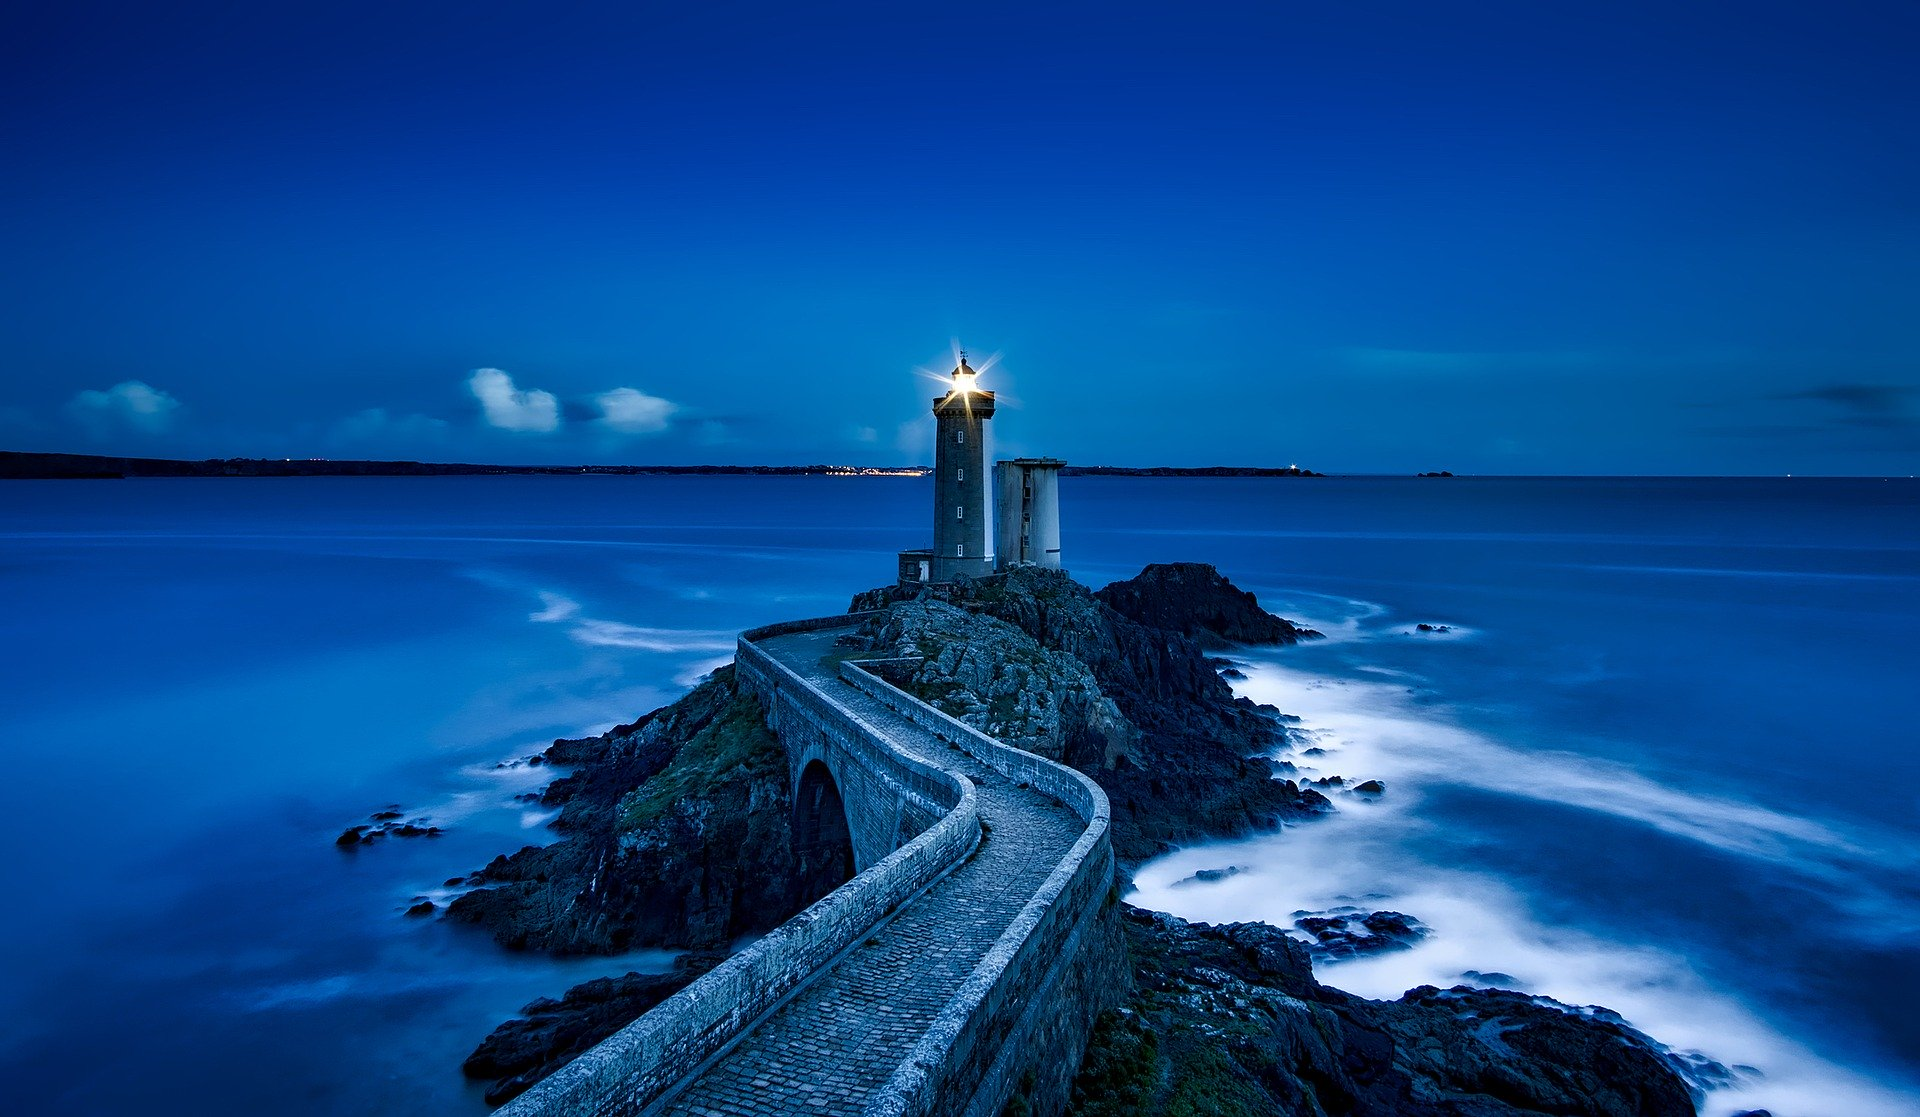
\includegraphics{images/plouzane-1758197_1920.jpg}
    \vspace*{40mm} %%% * is used to give space from top
    \begin{flushright}
        \textbf{\Huge {DevSecOps Tactical}}\\
        \vspace{5mm}
        \Large \textsf{Franklin Diaz}\\
        %\Large \textsf{Created on : April 20, 2020}
        \vspace*{0mm}
        %\Large \textsf{Last updated : \today}
    \end{flushright}
    \clearpage
    \vspace*{\fill}
\end{titlepage}
\justify{}
\textcopyright{} 2021, by Franklin Diaz
\justify{}
Licensed under \href{https://creativecommons.org/licenses/by-nc-nd/4.0/}{CC BY-NC-ND 4.0} 
\faCreativeCommons\ \faCreativeCommonsBy\ \faCreativeCommonsSa\
\vspace{5mm}\\
First Edition 2021
\justify{}
Front cover image design by {\href{https://www.linkedin.com/in/eddiemize/}{Eddie Mize}}.
Images at the beginning of the chapters in this book are
\href{https://pixabay.com/service/terms/#license}{courtesy of Pixabay}
\justify{}
The source for this book is available from 
{\href{https://github.com/thedevilsvoice/devsecops-tactical-book}{devsecops-tactical-book}}
\vspace{3mm}
Published on: \today
\justify{}
This book was initially drafted using the reStructuredText file format.
The Sphinx module for Python was used to format these files and programatically
generate LaTeX, and other working formats used in the typesetting process. The
resultant LaTeX files were managed using TeXstudio.
\justify{}
Some graphs have been generated programatically using the Graphviz software.
The entire publishing environment is developed and maintained according
to the principles outlined in this book.
\vspace{5mm}
\centering
\vspace{0mm}
\begin{figure}[!htb]
	\centering
	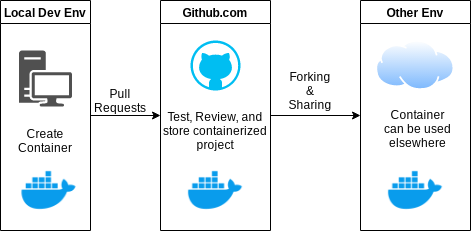
\includegraphics[scale=0.75]{images/workflow.png}
\end{figure}
\vspace{2mm}
Containerized publishing work flow.

\chapter*{Dedication}
\justify{}
This is where the dedication will be.
\chapter*{About the Author}
\addcontentsline{toc}{chapter}{About the Author}
\vspace{5mm}

\justify
Franklin Diaz is a Computer Scientist and lifelong computer hobbyist. He
spent 14 years as a Software Engineer, testing and developing Motorola's
CDMA cellular base station products. He spent five years Salesforce where
he was on the Security Detection Engineering team doing security log
aggregation and Data Engineering to augment and enhance the detection
capabilities of the Blue Team. 

Most recently he is at Palo Alto Networks where he works on the Professional
Services Team as a Principal Engineer with a focus on automation, Public
Cloud solutions and Continuous Integration and Deployment. He is also the
lead organizer for the BSides Indy security conference in Indianapolis, 
Indiana.

His education includes a Bachelor of Science in Computer Science from 
Roosevelt University, a Master of Science degree in Computer Information
Systems from Northwestern University, and a Master of Science degree in 
Network Security \& Network Engineering from DePaul University.
\vspace{5mm}

\chapter*{Preface}
\addcontentsline{toc}{chapter}{Preface}
\vspace{5mm}

\justify{}
Creation is a long and twisty path, fraught with the distractions of a life well-lived and the frenetic pace of a day and
age that clamors for a million tiny bits of our attention. A supportive and loving family is the touchstone that grounds
us through it all. The author would like to thank his family, especially his loving wife for making it possible to maintain
focus in a focus-stealing world.

\justify{}
Feedback has been a key component in getting these words organized into the order they appear before you today. Thank you to
those folks who contributed their time to review this book including Aaron Didier (@phreakinggeek).

\justify{}
A special thank you to {\href{https://www.linkedin.com/in/eddiemize/}{Eddie Mize} for providing the cover art for this book
and being a good friend.

\justify{}
The ideas captured here are not a means to any particular end. Rather, these are meant to be starting points, giving
you a frame of reference with novel technologies and techniques to streamline your workflows and give your projects
a productivity boost. The hope is the reader will gain momentum to pursue these new ideas by following along with the
examples outlined in this book.

\justify{}
You should work to build up your own solid base of code examples and problem solving techniques that will greatly increase
your efficacy. Over time, new tools and processes will rotate in and out of your toolbox as technology progresses. Keep
in mind that your job is to maintain that momentum, to keep experimenting and to see what is useful enough to stick with
you and make a permanent part of your technical repertoire.

\justify{}
This book is meant to be a workbook as much as it is meant to be read. You are encouraged to jump ahead, go back and re-read,
do the exercises you think you can apply the learning objective from right away, and skip the parts you don't think you will
ever use. Learning can be a non-linear experience and you are encouraged to ``color outside the lines'' to the extent you feel
comfortable doing so. That said, I've attempted to give this book a feel of moving the reader
along towards a final lab project. This project is meant to guide the reader through application of the topics covered before 
the final chapter.

\justify{}
Companies often make their services free in the hopes that you will see the value and usefulness of their products. Their
thinking goes that hopefully you will see enough utility that you will recommend them to your enterprise clients and
integrate their products into your workflows. Not a bad trade-off! It only makes sense to avail yourself of free-tier
cloud services, build and test platforms, and low or no-cost hosting environments. There are plenty of these out there and
we will explore some of these as we dive further into the topics.

\justify{}
When we choose to use a tool, say Ansible\index{Ansible} for example, we must adopt the
most up-to-date and best practices for using that tool. File system layout, naming conventions, script syntax and organization,
and so on. We get to enjoy the clear and safe path forged by the folks that came before us, and with whom we share many goals.
As your skills mature over time, you may want to consider donating time back to the
open source and other communities upon which your knowledge has been built.

\justify{}
Finally, I find it very helpful for my own personal peace of mind to leave projects ``clean and green'', to the extent
possible. In other words, there is mental benefit to tidying up your physical and virtual workspace
before walking away from the keyboard for the day. Perhaps you would find similar benefit should you choose to adopt
this practice.
 %preface and acknowledgements
\tableofcontents
\listoffigures
\listoftables

% mainmatter: parts and chapters
\mainmatter
\chapter{Introduction}

\centering
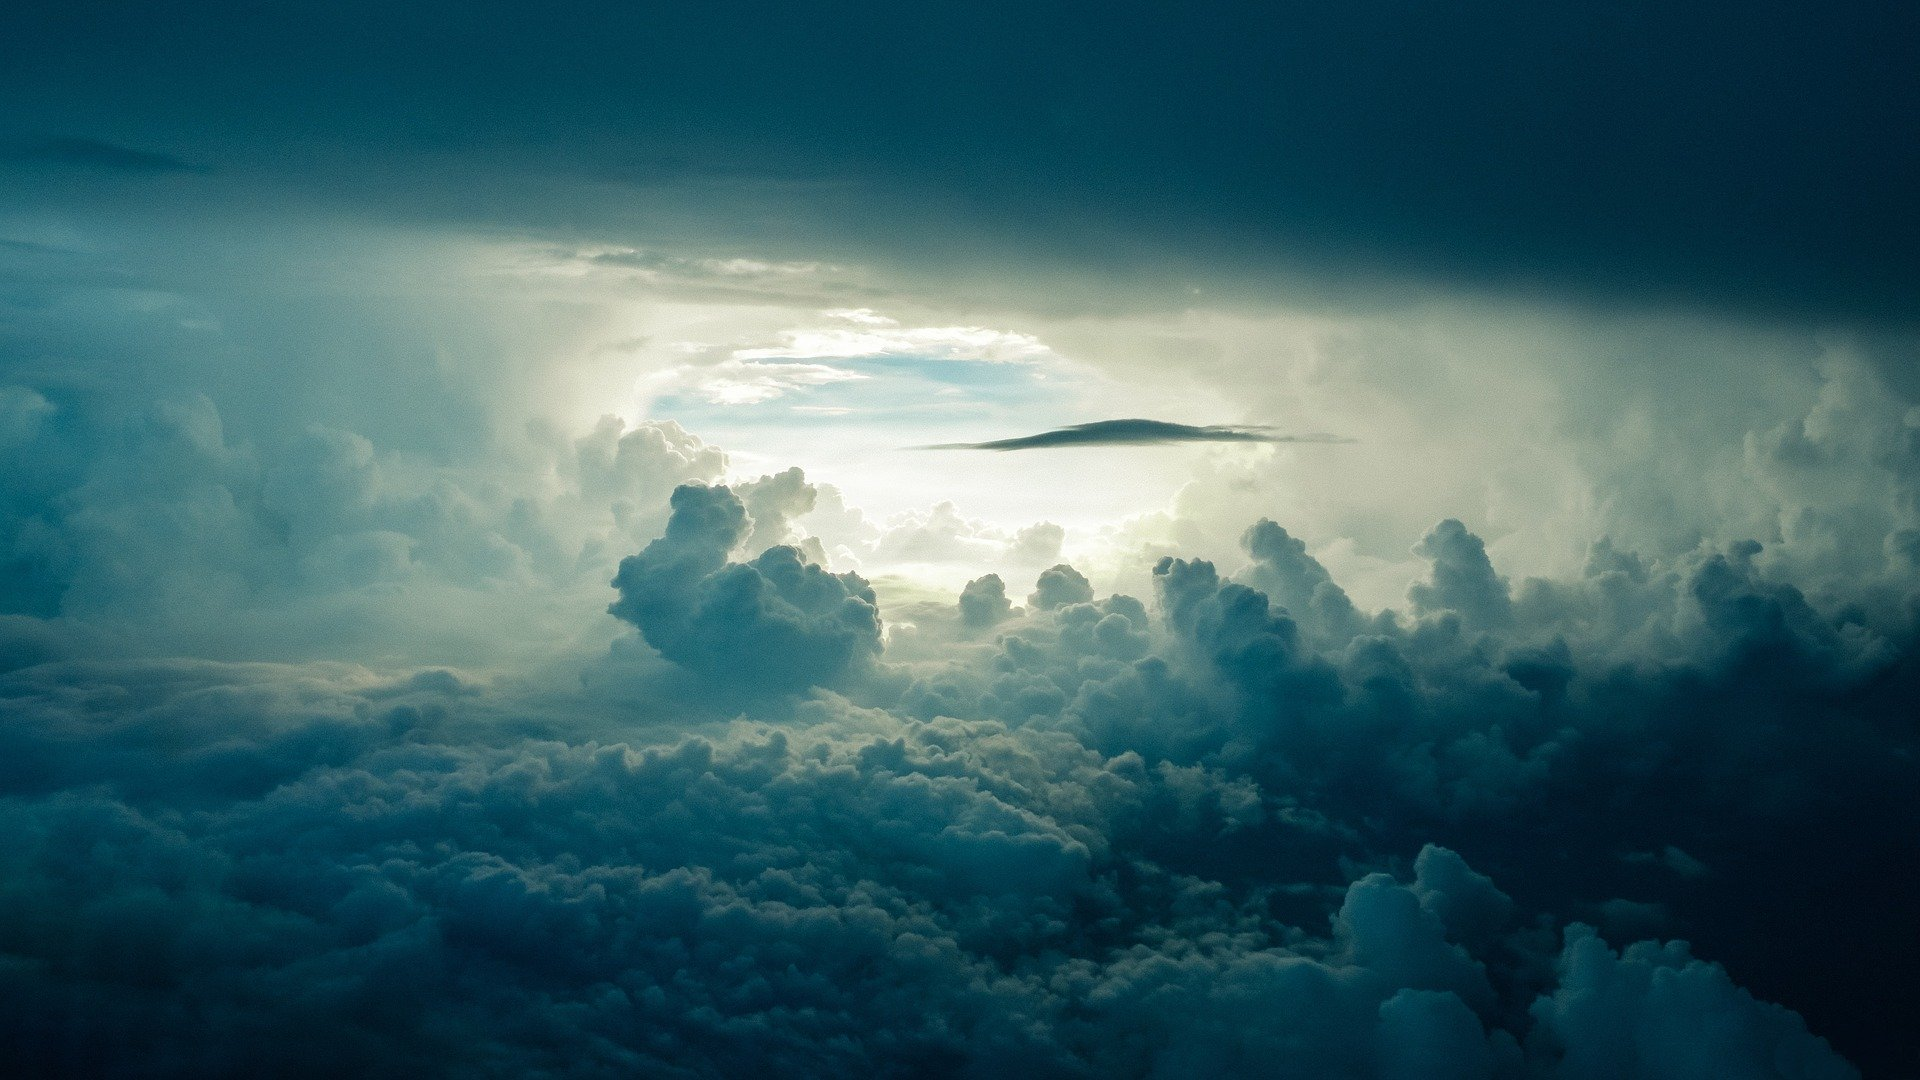
\includegraphics{../images/sky-690293_1920.jpg}

\justify{}
The term DevSecOps\index{DevSecOps} is an amalgam of the words Development, Security,
and Operations. The combination of these three words represents the overlap and
interplay between sometimes disparate work functions. The degree to
which these three realms overlap is often a reflection of the structure of a given
organization. Simply put, DevSecOps lives at the intersection of application development
and/or Infrastructure as Code development, Information Security, and Network Operations.

\justify{}
This overlapping DevSecOps job functionality has some overarching goals For
example, the movement software through an ongoing series of incremental test and
deployment phases, which is often referred to as pipelines\index{pipeline}. We will
explore this concept of pipelines and other ways our platforms and infrastructure
are becoming more abstract from the viewpoint of the tools that we use to do it.
Definition of our infrastructure in reusable software patterns is another big objective
in the DevSecOps paradigm. This Infrastructure as Code 
(IaC)\index{Infrastructure as Code (IaC)} is the platform
upon which our application software work products flow through a cycle of Continuous
Deployment or Continuous Delivery (CD)\index{Continuous Delivery (CD)}.

\justify{}
Folks at the leading edge in today's computing industry are not just building
software, but are curating it through a cyclical process of continuous development,
testing, use, and improvement. With increasing frequency, applications and
workloads are moving to computing environments that are abstracted away, managed
by invisible armies of engineers who work at companies other than their own. Of course
we are referring to those multitenant cloud type computing landscapes. Passing
one or more fully encapsulated applications to a cloud provider for the purposes
of having ``someone else'' host it as a production environment has become
commonplace. Further, cloud service providers are adding new features and capabilities
at breakneck speed. We are promised our staff will be liberated from burdensome
maintenance tasks for hosts, networks, traffic capacity, storage, and more once
e decide to go ``Cloud Native''. Large amounts of time,
money, and resources are being thrown at cloud migration efforts. Moving away
from traditional networks to those hosted in public
cloud provider environments takes plenty of time, money, planning, and refactoring.
The world is changing with respect to how software is created and maintained.

\begin{figure}[!htb]
	\centering
	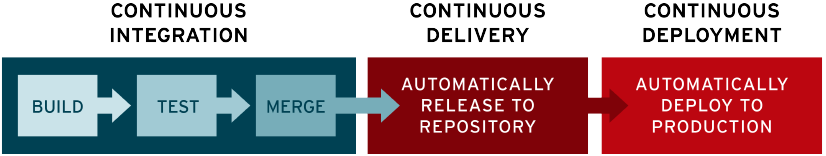
\includegraphics[scale=0.35]{../images/ci-cd-flow-desktop_0.png}
	\caption{Typical pipeline stages.}
\label{stages}
\end{figure}

\justify{}
To the extent possible, the modern software project team often aligns around an
attempt to realize gains in performance of our people and projects by
leveraging automation\index{automation} and Agile development practices throughout the
feature development cycle. We aim to reduce complexity, increase consistency, and make
scaling up as smooth as possible, all at once.

\justify{}
At the time of this writing in 2020, about 40\% of production workloads are
running on containers or are deployed in low cost serverless configurations.
Bare metal and virtual machines currently host a bit over 60\% of production
workloads. Containerized workload use is expected to increase even more in
the coming years. Conversely, bare metal and VM usage is expected to
decrease in the coming years.\cite{cnative}

\justify{}
It's not a question of if, but how quickly commoditization of compute resources
will replace private corporate data centers, perhaps resulting in only a
few main providers of cloud computing resources. This shift has been likened
to how power generation and distribution became centralized
in the previous century, now the domain of a few large utility companies.
Nothing beyond considerations of time, money, and practicality stop you
from making your own electricity, but most folks are keen to invest their
efforts in other pursuits.

\justify{}
Strategic decisions are about defining the direction of a team and overseeing
the allocation of the resources needed to pursue the goals of the entire
business organization. These are the sorts of things the upper managers are
thinking about. The linking of the strategic direction to tactical tasks is
done with operational planning. This managerial view might be best framed in
year-long increments. Think of operational planning as the purview of line
and middle managers who detail the goals and milestones, and capture metrics
on progress toward strategic goals of the business. Finally, tactical concerns
are the short range objectives of a team within a department or business unit.
The tactical viewpoint tends to span a time period of one year or less and is
the domain of the individual contributor and technical champion. This is the
``fun stuff'', where you get to be closest to the code. This book will focus
on the practical, by and for those who want to be tactical. There is also
an interdependence on the logistical here. Logistics in our context refers to
the things that make it possible for the tactical to succeed, and look good
while doing it!

\justify{}
Among the tactical practitioners, we can further decompose responsibility into
varying degrees of Development, Security, and Operational work. The typical
person in a developer type role is often working under stringent deadlines to
``ship code'', which means their main focus is ``getting code out the door'' to
keep management happy. Folks in a role that is mainly security focused are mostly
concerned with prevention of the abuse of the technology assets of a business. The
operations type roles have the task of keeping everything up and running, as well as
ensuring all the bits and pieces of technology functioning properly together.

\justify{}
In this book, we will explore a combination of techniques that can enhance and refresh
your skills and align your projects with the technological leading edge. We will
introduce various popular technologies, then use common bits and pieces of
these technologies to get you thinking like a DevSecOps practitioner. We will try out
various code snippets and exercises to build confidence. The ultimate goal is to be able to
create a secure build pipeline for your lab and development work,
test, and even production environments. The techniques here are meant to help
the security-minded developer sharpen her or his skills, and introduce tips
and tactics that benefit the teams they are a part of. There are many, many
ways to reach similar goals these days with the preponderance of Open Source
and commercial tools that are available. By focusing on a few we can blaze a
trail to success in our projects.

\justify{}
Often a distinction is made between folks
who work on the front and back end of software ecosystems. It should be noted that this
book is written by someone with the
experience and perspective of a ``backend'' developer.

\justify{}
We have a goal in mind of selecting complementary tools and process to construct
and streamline our ways of working. We will attempt to leverage these ways to
get us quickly and securely to a working example lab environment. Along the
way we should strive for simplicity and reduction of complexity when possible.
Experience tells us that tools, security measures, and process that are too cumbersome
or otherwise prohibitive in nature are typically circumvented, or even abandoned.
Complexity in our processes become the snags and side projects that are the
enemy of productivity.

\justify{}
Refuse to shave more yaks\cite{yak} than absolutely necessary!

\chapter{Some Big Ideas}


\includegraphics[scale=0.85]{../images/book-5104342_1920.jpg}

\justify
There are some key precepts that will serve the aspiring DevSecOps
engineer well. In this chapter we will explore some of these in
an attempt to levelset our understanding of the domain. We will also
continue to introduce the reader to the vernacular
of the modern day DevSecOps engineer in a world gone cloudy.

\section{Piplines (a.k.a. The Flow)}

\justify
Code, documents, test cases, and other software work products begin
their life on developer workstations. In this book we will refer to
the environments where this takes place as the "local" environment. 
These work products are created, reviewed and checked into Revision 
Control Systems (RCS)\index{Revsion Control System (RCS)}, 
GitHub\index{GitHub} for example, by the DevSecOps practitioner. 
Other revision control systems include GitLab\index{GitLab} and 
BitBucket\index{BitBucket}.

\justify
We will delve into various types and spects of testing 
throughout this book. For now it is enough to understand the idea of
a test case as a discrete check, or grouping of similar types of 
checks, that we use to ensure our work products meet certain minimum
standards.  Test cases are created with and often run against our
work products at the time they are checked in to the revision control
system. This is meant to ensure stability, security, and compatibility
with the existing code base in revision control. The automation required 
to execute tests every time work is checked in to revision control is 
typically the responsibility of the DevSecOps engineers. As seen in 
figure \ref{fig:pipeline}, work typically "flows" from the local environments, 
into a test environment, and finally to production where it is available 
for use by the entire user base.

\begin{figure}[!htb]
	\centering
	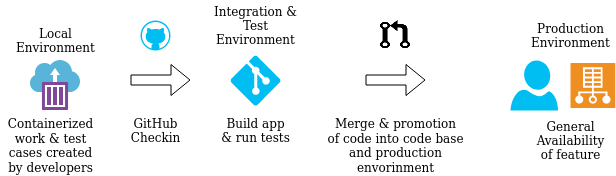
\includegraphics[scale=0.63]{../images/flow.png}
	\caption{Typical build pipeline.}
	\label{fig:pipeline}
\end{figure}

\justify
We will refer to the entirety of this three-stage flow as one example of
a "build pipeline"\index{pipeline}. Code from one or more local environments is checked in to
the revision control system throughout a typical DevSecOps workday, and
continuously tested and integrated with the main code base. That is to
say, work undergoes "Continuous Integration" (CI)\index{Continuous Integration (CI)}
with the main code base, and often "Continuous Delivery" (CD)\index{Continuous Delivery (CD)}
between local, test, and production environments. This is where the term
"CI/CD Pipeline" comes from. A business unit may choose to designate more
than just the three "dev", "test", and "prod" environments mentioned here,
depending on their particular use cases and ways of working. 

\justify
While the CI/CD Pipeline is often the primary focus of the DevSecOps
engineer, other pipelines exist as well. For example, let's assume our
organization maintains a vast pool of raw data, also known as a data
lake\index{Data Lake}. The staff Data Engineers build and maintain 
Data Science\index{Data Science} pipelines to facilitate the smooth flow
of logs and other data into that data lake. Now Data Scientists are able
to create machine learning models that rely on that data to produce useful
insights. As another example, consider code changes as they move from
developer workstations into a code repository for storage. Accessing
this code for the purpose of testing will differ from how it is accessed
for the purposes of deployment. The order of operations and flow
between differing functions might be said to comprise two different pipelines.

\section{Shifting Left}

\justify
We now have a mental picture of how software will flow through our
three environments, from Development, to Test, and finally into Production
where it is accessible to the widest base of consumers. Integration of 
best security practices into this flow, as early and as often as possible, 
is highly desirable. 

\justify
Imagine our software life cycle occurring along a temporal 
axis, t. Intentionally moving security to the left on this axis (lower 
values of t) is known as "Shifting Left"\index{Shift Left} as seen in 
figure \ref{fig:shift}.

\justify
\begin{figure}[!htb]
	\centering
	\begin{tikzpicture}
	  \draw[<-,thick,black!10!blue](2.0cm,\nOne) -- (7.0cm,\nOne) node[midway,below]{security};
	  \draw [->, ultra thick] (0,0) -- (10,0) node[pos=0, below]{t=0} node[pos=0.5,below]{software lifecycle (time t)} node[pos=1, below]{t=n};
	\end{tikzpicture}\\
	\caption{Shifting security to the left.}
	\label{fig:shift}
\end{figure}

\justify


\section{Zero Trust}

\section{Automation}

\justify
Consider what may happen when we want to apply the lessons from this book across a large environment made up of many hosts, containers, pieces of application software, etc. It becomes a huge challenge for an operator to log in to each host or container individually. Typing, or even cutting and pasting commands to keep things up and running properly, look at logs, and so on becomes problematic. Creating shell scripts can be quite helpful, but is an outdated modality when we consider the daunting size and complexity of the modern administrative domain.

\justify
This is where automation comes in. Automation\index{automation} is a way to provision and maintain some or many hosts in a programmatic manner. Another desirable goal, and hopefully result of automation is to reduce the amount of per-host interaction that comes with the work of administering systems. Automation is the force multiplier we use to achieve scaling\index{scaling}. Couple this precept with the explosive automation tooling ecosystem and you are on the path to doing more, better work in less time with a smaller staff. 

\section{Ephemerality}

\justify
Ephemerality/index{Ephemerality} is the concept of something being transitory in nature,
existing only briefly\footnote{\url{https://en.wikipedia.org/wiki/Ephemerality}}.
Using immutable containers makes it easier to realize infrastructure and
hosts that are ephemeral. Rather than spending a great deal of time
patching and upgrading one or more hosts as we might in a traditional
project stack that uses virtual machines or bare metal, we're going to
use Docker to create a new container in place of the old one. In other
words, we're running our project in containers that are immutable and
ephemeral to the degree possible.

\section{Immutability}

\justify
There is obvious advantage of being able to quickly stand up new clones
of our project to replace existing instances that may be outdated,
insecure, etc. The idea of immutability\footnote{\url{https://www.hashicorp.com/resources/what-is-mutable-vs-immutable-infrastructure/}},
in reference to software projects, is the degree to which something, our
running project for example, can be changed. Immutability\index{Immutability} is desirable,
in that we wish to be able to simply replace outdated instances of our
project in their entirety. Upgrading and patching are inherently
problematic activities, high cost in terms of time, effort and money,
that we have the technology to dissociate from. With containerization,
we can more easily achieve immutability across the software life cycle.

\section{Agile Methodologies}

\justify
The concept of Agile\index{agile} Software development is an expansive topic unto itself. Although we won't implicitly dedicate a lot of our time to these ideas, agile is widely regarded as an underpinning of a successful
DevSecOps program.
\chapter{Getting Ready to Get Tactical}

\centering
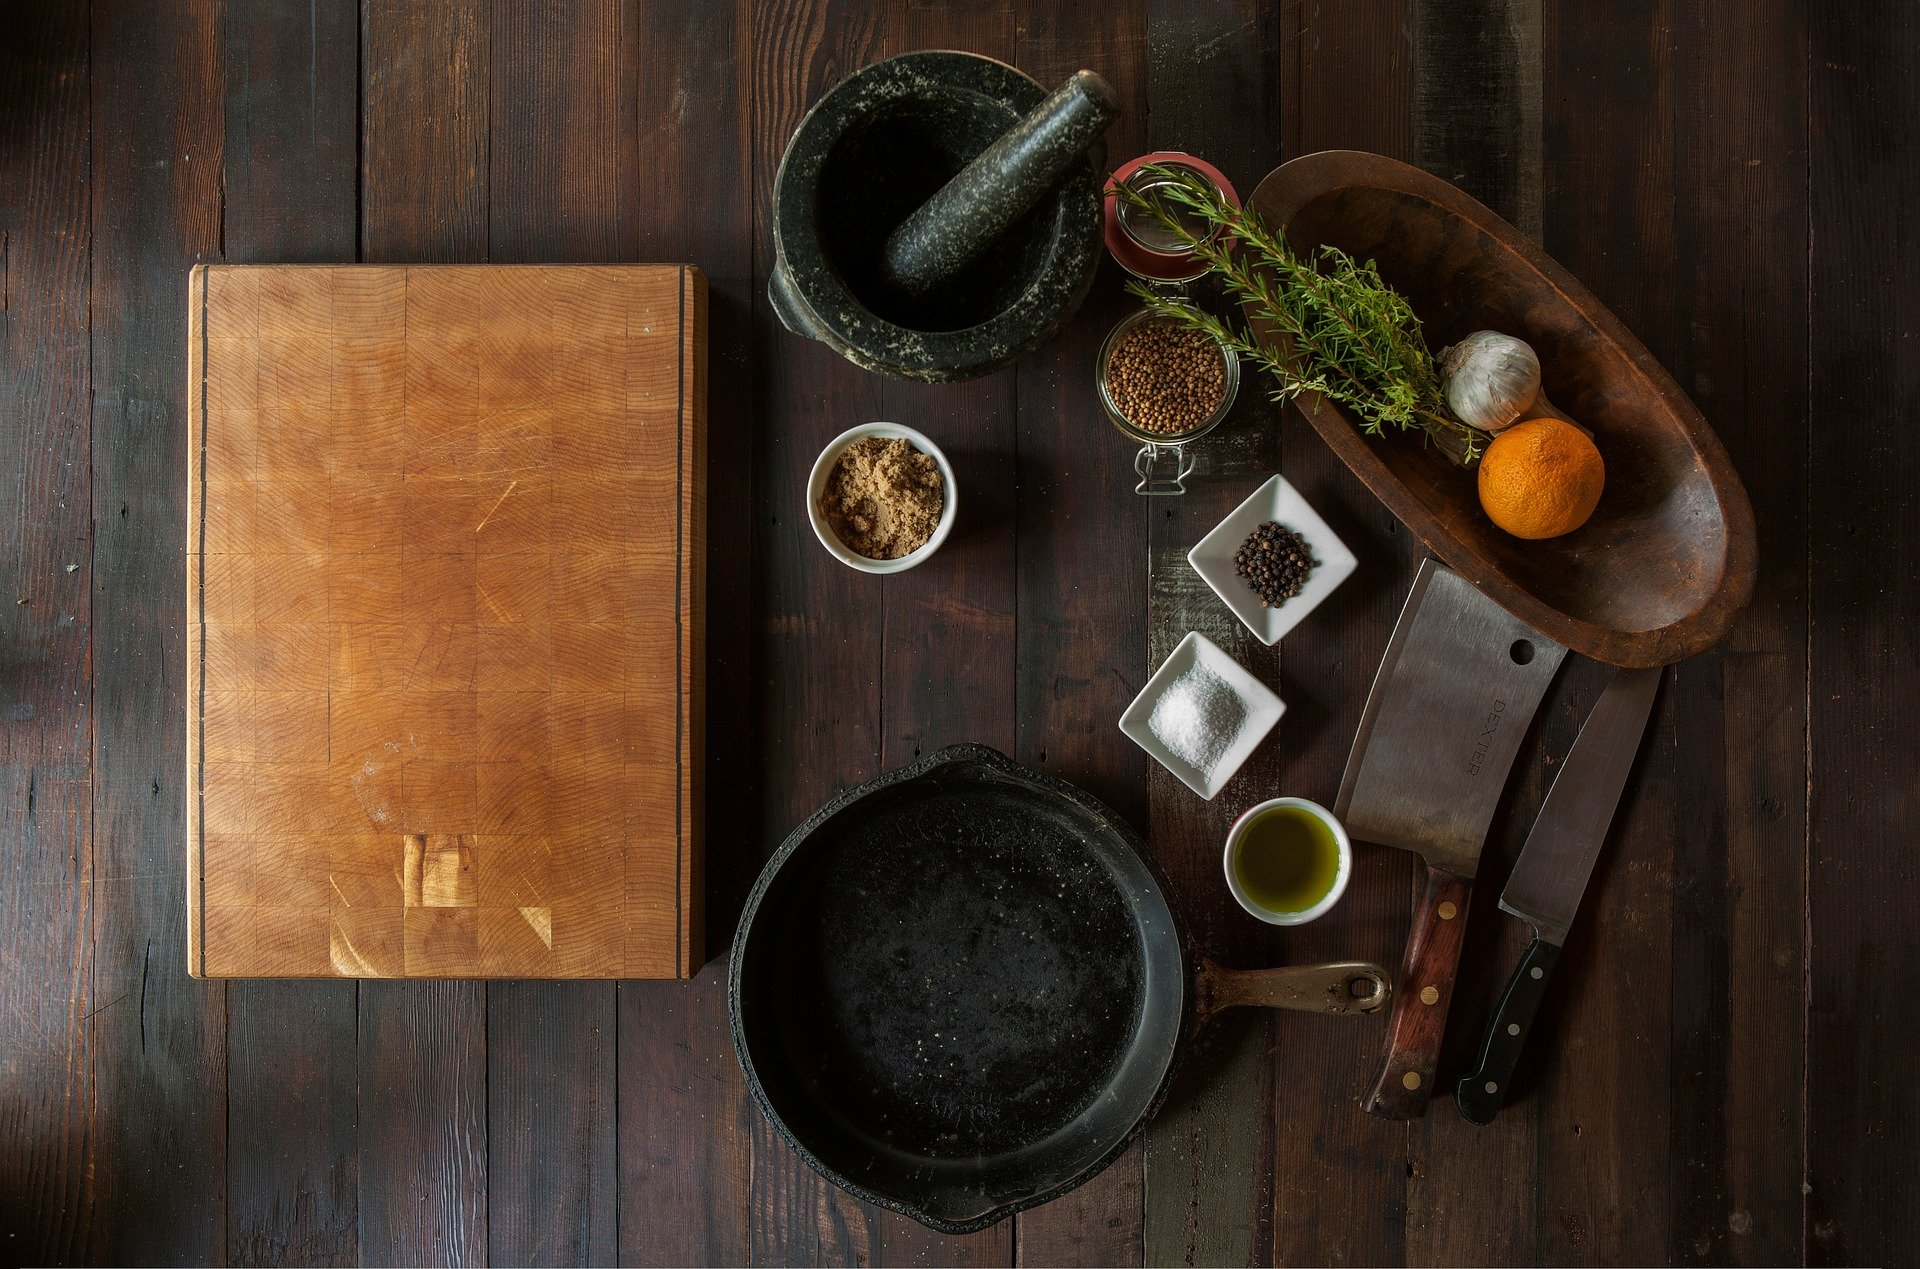
\includegraphics[scale=0.20]{images/ingredients-498199_1920.jpg}


\justify{}
Think of this chapter as the \emph{mise en place} of our DevSecOps souffle. We will increase our chances of success
by preparing our work environment for the project at hand. Let's start our preparations by outlining our
overall objectives. We want to:

\justify{}
\begin{itemize}
	\item
	      Create an extensible lab environment for rapid prototyping and development.
	\item
	      Keep our lab costs down while meeting the rest of the objectives.
	      Utilize free services and open source tools to the extent possible.
	\item
	      Use the published best practices for each tooling, operations, or
	      development ecosystem we choose to employ.
	\item
	      Always leave our projects in a functional state.
	\item
	      Get out of our old comfort zone, into a new one.
\end{itemize}

\section{Prerequisites}

\justify{}
This book intends to be a practical treatment of common and popular technologies from the DevSecOps world. As such, we assume
the reader has some basic knowledge of certain concepts. We will be exploring new ways of working for folks who
are somewhat familiar with:

\begin{itemize}
	\item
	    Linux (UI and command line)
	\item 
        Python 3
	\item
	    Familiarity with github.com and the concepts of pull requests and branching.
\end{itemize}

\justify{}
The examples in this book have been tested on Linux running the latest version of Docker. Let's take a look at some
of the other foundational environmental elements we need in place to be successful.

\section{Packages}

\subsection{Macintosh}

Using ``brew'' and ``cask'' to install and manage packages on Mac will make your life much simpler.

\subsection{Linux}

My prefered environment is a Debian based distribution. Ubuntu, Cinnamon, and PopOS are all examples of 
Linux distrubutions in this family.

\section{The Workhorse (IDE)}

\begin{figure}[!htb]
\centering
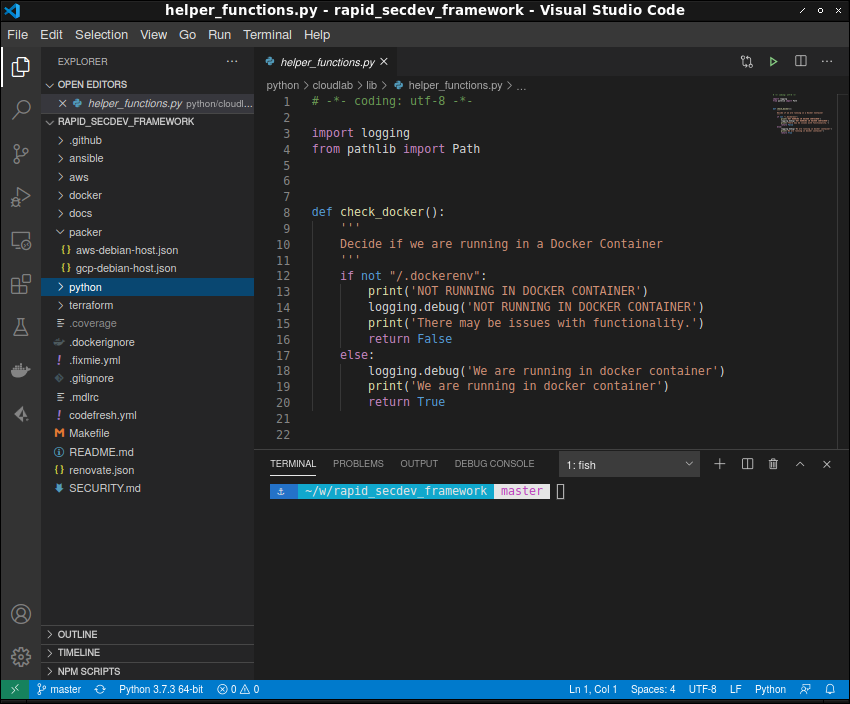
\includegraphics[scale=0.45]{images/setup-vscode.png}
\caption{The VScode IDE.}
\end{figure}

\justify{}
It is quite helpful to have a piece of software on your workstation that makes code and document creation and edits easier. This
software is commonly known as an Integrated Development Environment (IDE)\index{IDE}. A decent IDE with the right add-ons can
provide syntax highlighting to show potential issues you might have missed, help you check for spelling or
grammar mistakes in your documentation, and even makes suggestions on alternate ways of writing your code.

\justify{}
There are many commercial and Open Source IDEs available. Visual Studio Code from Microsoft is a popular choice due to it's easy
installation. VSCode\index{VSCode} works well on Linux, Mac and other operating systems.
The environment is easily extensible to support most any language, linter, or syntax checker we may have a need
for, thanks to their easy to use and well integrated ``Extension'' feature. VSCode also has an integrated terminal
window\index{Terminal Window} so the developer can execute shell commands without leaving the IDE screen.

\section{SSH Key Setup}

\justify{}
Take note of the fact that setting up SSH keys means generating a pair of keys, not a single key. This is an important 
distinction. You will want to add your public key to sites like \href{github.com}{github.com}. The public key half will
also be added to machine instances that you create with public cloud providers. This will allow you to log in without
having to provision a user/password combination. You should take care to 
protect the private key at all times. Under no circumstances should you share your private SSH key.\cite{ssh}
\justify{}
Take a few minutes to generate an SSH key\index{SSH keys} pair if you don't already have one. We will add the public half of
our SSH key pair to hosts we provision. The directions for generating an SSH keypair found on the
\href{github.com}{github.com} website are perfect for our setup task. Follow the directions in the article 
\href{https://docs.github.com/en/github/authenticating-to-github/connecting-to-github-with-ssh/generating-a-new-ssh-key-and-adding-it-to-the-ssh-agent}{Generating a new SSH key and adding it to the ssh-agent}

\subsection{Generating a Key from the Command Line}

If you are using a Linux or Mac system, you have the option to create your SSH key pair from the command line. Consider 
the following example code listing.

\begin{mybox}{\thetcbcounter: SSH Key Generation}
\lstinputlisting{code/03_setup/ssh-key-generation}
\end{mybox}

\justify{}
Now you can add your public key half to your user settings in \href{github.com}{github.com}. For me it makes sense to have
two key pairs, one used for work projects, and one used for personal projects.

\section{GPG Key Setup}

\justify{}
\href{https://gnupg.org/}{Gnu Privacy Guard (GPG)} is an Open Source replacement for Symantec's PGP software. It allows you
to generate an asymmetric key pair that can be exchanged with other users, encrypt your personal files, or verify your identity.
Again, you will want to be sure to share your public key and protect your private key. This is the same reasoning we used in the
case of our SSH keys.

\justify{}
We will use a GPG key to sign commits to GitHub\index{GitHub}. This will help others verify that work you check in to revision
control did actually come from you. It's not strictly necessary but is considered good practice.
Some repositories require that you sign your pull requests with your GPG key\index{GPG key}.

\justify{}
Take a few minutes to set up a GPG key. Once you have an account setup, you can add
it to your profile on \href{github.com}{github.com}.

\subsection{Command Line GPG Key Setup}

\begin{mybox}{\thetcbcounter: Command Line GPG Key Setup}
\lstinputlisting{code/03_setup/gpg-key-setup}
\end{mybox}

\justify{}
Copy your GPG key, beginning with the string ``BEGIN PGP PUBLIC KEY BLOCK'' and ending with the string
``END PGP PUBLIC KEY BLOCK''. Add the GPG key to your GitHub account.

\section{Using pass to Encrypt Secrets Locally}

\justify{}
The pass program allows you to encrypt your keys, files, and other secrets in an encrypted database that is
stored in your home directory. Know that eventually, secrets leak. They can be exposed in a variety of ways, 
often they are committed to revision control by mistake.

\begin{mybox}{\thetcbcounter: Encrypt Local Secrets}
\lstinputlisting{code/03_setup/pass-mgr}
\end{mybox}

\part{Development}
\chapter{Containers}

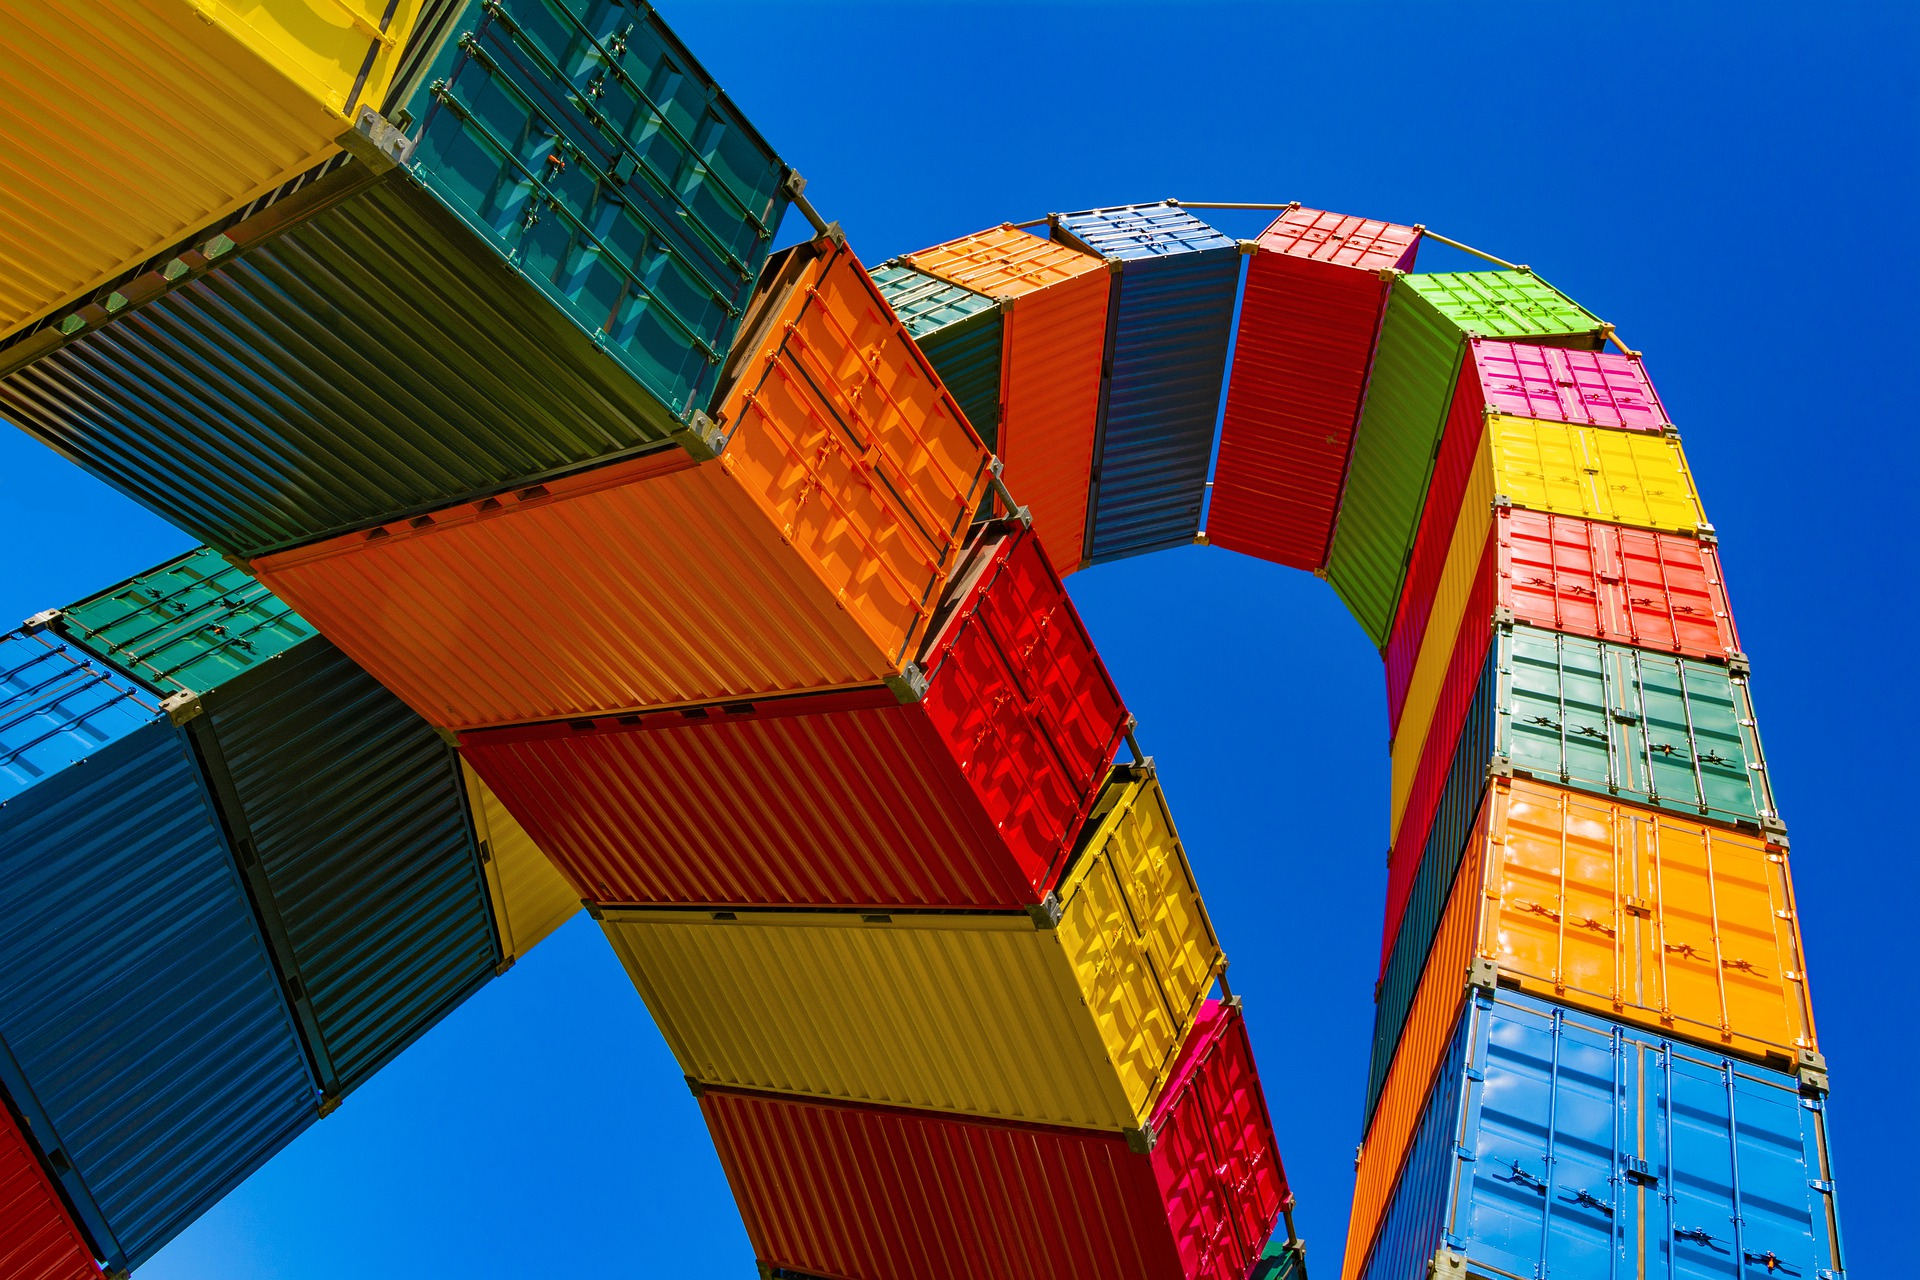
\includegraphics[scale=0.85]{../images/container-4203677_1920.jpg}

\justify
Containerization is the process of generating a fully functioning
software ecosystem that includes code and dependencies for part or all
of a project. The most popular and common tool for realizing
containerization is Docker\index{Docker}. Using Docker, we can programatically build
an environment for our project, and pass the entirety of this
encapsulated environment from our local development machine, into the
Continuous Integration (CI)\index{Continuous Integraion} pipeline for testing, and eventually into
our production environment. Containerization\index{containerization} helps us by offering a
consistent operating experience across disparate environments.

\justify
It is more desirable to create projects that are built and replaced
frequently, than it is to attempt to upgrade and repair the
infrastructure, platforms, and project code. Attempts to patch and
upgrade project hosts "in place", such as with bare metal platforms for
example, quickly reveal great difficulty in maintaining consistency with
the project source. This also introduces issues keeping operating system
packages current, yet still compatible with the project. Imagine a situation where an upgrade to a package is necessary to meet security requirements, but this very same upgrade means the project stop working
since the package features have also changed. The result is most likely
angry end users and customers. Certainly not a situation we ever like to
find ourselves in.

\justify
Docker images are "canned" (as in, prefabricated) or custom directives
for provisioning the operating system of a Docker container. One or more
images can be used as building blocks when configuring our containers.
For example, a base Linux image and base Python image might be combined
with our customizations that describe and point to our application code,
all of which make up a single containerized "server". We get the added
benefit of being able to switch quickly between base operating system
images with just a few lines of code change to our project. For example,
we could easily modify our container image to be predicated on Debian
rather than Red Hat distribution of Linux kernel and operating system
should the need arise.

\justify
See the Docker website for instructions on how to install and configure
Docker. A properly
functioning Docker setup on your local machine is a requirement for the
exercises we will do later. Note that Podman is an acceptable substitute
for Docker, as detailed later in this chapter.

\justify
Once you have Docker installed and running on your workstation, take a
look at the two example files below. For now it's OK to see them and get
a general familiarity with their contents. Later we will use these files
to create containers for our projects.

\section{Dockerfile}
\justify
The Dockerfile is our basic unit of containerization. That is to say,
our containers, and the applications they contain, are defined by the
Dockerfile. This Dockerfile will dictate how we provision resources and
include operating system essentials and packages inside our container.
Each Dockerfile is predicated on a base image, such as Python/Debian 10
as shown in the example below.

\justify
Consider a directory named
\href{https://github.com/hotpeppersec/rapid_secdev_framework/tree/master/docker}{Docker}
and a file called
\href{https://github.com/hotpeppersec/rapid_secdev_framework/blob/master/docker/Dockerfile}{Dockerfile}\index{Dockerfile}
within this directory. Note the capitalization of the first letter in the file name. Some IDE's will key off this file and allow for additional syntax highlighting.

\justify
\begin{mybox}{\thetcbcounter: Dockerfile}
  \lstinputlisting{code/04_docker/Dockerfile}
\end{mybox}


\justify
A valid Dockerfile begins with the \textbf{FROM} instruction. This
instruction specifies the base image that we will use to build our
project on. These base images come from the
\href{https://docs.docker.com/docker-hub/repos/}{Docker Hub
  repositories}. We are setting an environment variable
\textbf{DEBIAN\_FRONEND} to the value of noninteractive, which will
cause the apt command to skip or ignore any interactive menus that are
encountered during execution of the apt command, since these would cause
our builds to "hang up" at an inaccessible interactive prompt. The
\textbf{ADD} and \textbf{WORKDIR} directives are meant to cause Docker
to use the /workdir directory as the root of the project "inside" the
container. Finally, we are directing Docker to \textbf{RUN} and apt
update and install the apt-utils package.

\subsection{docker-compose.yml}
\justify
The docker-compose tool and its associated docker-compose.yml file
allows us to manage multiple Docker containers for one or more
applications. We will add this file to our project to illustrate it's
composition and give ourselves the ability to extend our work later, as
needed.

\justify
A file called docker-compose.yml\index{docker-compose.yml} will exist alongside our Dockerfile in our docker directory.

\begin{mybox}{\thetcbcounter: Example docker-compose.yml}
  version: '3'\\
  services:\\
  \hspace*{7mm}devsecops:\\
  \hspace*{15mm}hostname: devsecops\\
  \hspace*{15mm}container\_name: devsecops\\
  \hspace*{7mm}volumes:\\
  \hspace*{15mm}- ..:/project\\
  \hspace*{7mm}build:\\
  \hspace*{15mm}context: ..\\
  \hspace*{15mm}dockerfile: docker/Dockerfile
\end{mybox}

\justify
The docker-compose.yml file begins with a version specification. It's
important to note that the commands and structure of docker-compose.yml
can vary widely based on this version. While versions cannot be mixed,
all version are valid with respect to docker-compose itself. Wew specify
a service named "devsecops", and assign a host and container name. Under
"volumes" we are mounting the base of the project directory in the host
filesystem as "/project" in the container filesystem. The build
"directive" tells docker-compose how to locate the Dockerfile we wish to
use for the containers.

\subsection{Exercise: Testing Out Docker}
\justify
With Docker properly installed and an understanding of the necessary
configuration files, we can now try out our configuration. See
({myFig1}) for an illustration of how to lay out the project files in your local filesystem.


\begin{figure}[!htb]
  \centering
  
\begin{tikzpicture}[>=latex,line join=bevel,]
  \pgfsetlinewidth{1bp}
%%
\pgfsetcolor{black}
  % Edge: home -> devsecops
  \draw [->] (96.5bp,215.7bp) .. controls (96.5bp,207.98bp) and (96.5bp,198.71bp)  .. (96.5bp,180.1bp);
  % Edge: devsecops -> github
  \draw [->] (85.871bp,143.7bp) .. controls (80.872bp,135.56bp) and (74.809bp,125.69bp)  .. (64.007bp,108.1bp);
  % Edge: devsecops -> gitignore
  \draw [->] (107.38bp,143.7bp) .. controls (112.49bp,135.56bp) and (118.7bp,125.69bp)  .. (129.75bp,108.1bp);
  % Edge: github -> codeowners
  \draw [->] (53.5bp,71.697bp) .. controls (53.5bp,63.983bp) and (53.5bp,54.712bp)  .. (53.5bp,36.104bp);
  % Node: home
\begin{scope}
  \definecolor{strokecol}{rgb}{0.0,0.0,0.0};
  \pgfsetstrokecolor{strokecol}
  \draw (123.5bp,252.0bp) -- (120.5bp,256.0bp) -- (99.5bp,256.0bp) -- (96.5bp,252.0bp) -- (69.5bp,252.0bp) -- (69.5bp,216.0bp) -- (123.5bp,216.0bp) -- cycle;
  \draw (96.5bp,234.0bp) node {/home};
\end{scope}
  % Node: devsecops
\begin{scope}
  \definecolor{strokecol}{rgb}{0.0,0.0,0.0};
  \pgfsetstrokecolor{strokecol}
  \draw (157.5bp,180.0bp) -- (154.5bp,184.0bp) -- (133.5bp,184.0bp) -- (130.5bp,180.0bp) -- (35.5bp,180.0bp) -- (35.5bp,144.0bp) -- (157.5bp,144.0bp) -- cycle;
  \draw (96.5bp,162.0bp) node {/home/devsecops};
\end{scope}
  % Node: github
\begin{scope}
  \definecolor{strokecol}{rgb}{0.0,0.0,0.0};
  \pgfsetstrokecolor{strokecol}
  \draw (84.0bp,108.0bp) -- (81.0bp,112.0bp) -- (60.0bp,112.0bp) -- (57.0bp,108.0bp) -- (23.0bp,108.0bp) -- (23.0bp,72.0bp) -- (84.0bp,72.0bp) -- cycle;
  \draw (53.5bp,90.0bp) node {.github};
\end{scope}
  % Node: gitignore
\begin{scope}
  \definecolor{strokecol}{rgb}{0.0,0.0,0.0};
  \pgfsetstrokecolor{strokecol}
  \draw (178.5bp,108.0bp) -- (102.5bp,108.0bp) -- (102.5bp,72.0bp) -- (178.5bp,72.0bp) -- cycle;
  \draw (140.5bp,90.0bp) node {.gitignore};
\end{scope}
  % Node: codeowners
\begin{scope}
  \definecolor{strokecol}{rgb}{0.0,0.0,0.0};
  \pgfsetstrokecolor{strokecol}
  \draw (107.0bp,36.0bp) -- (0.0bp,36.0bp) -- (0.0bp,0.0bp) -- (107.0bp,0.0bp) -- cycle;
  \draw (53.5bp,18.0bp) node {CODEOWNERS};
\end{scope}
%
\end{tikzpicture}


  \caption{Project Directory and Docker related files.}
\end{figure}

\clearpage
\justify
Here is a step by step description of how to prepare the creation of our first container:

\begin{itemize}
  \item Create the "rapid\_secdev\_framework" folder.
        \begin{itemize}
          \item When creating folders, note that capitalization matters.
        \end{itemize}
  \item In that folder, create another folder called "docker".
  \item Now in the docker folder, create a text file with the name "Dockerfile".
        \begin{itemize}
          \item
                Copy and paste the example Dockerfile from earlier in this chapter
                into your text file.
        \end{itemize}
  \item Also in the docker folder, create a text file with the name "docker-compose.yml"
        \begin{itemize}
          \item Copy and paste the example docker-compose.yml file from earlier in this chapter into your second text file.
        \end{itemize}
\end{itemize}

\justify
Here is an example of the BASH shell commands you can use to accomplish
the steps of the exercise. You can substitue vi for your favorite text
editor as needed. Note that typing the "docker-compose" command on line
6 will reference the devsecops "service" we specified on line 3 of the
docker-compose.yml file.

\justify
\begin{mybox}{\thetcbcounter: Create files for Docker,height=3.5cm}
  mkdir rapid\_secdev\_framework\\
  cd rapid\_secdev\_framework\\
  mkdir docker\\
  vi docker/Dockerfile\\
  vi docker/docker-compose.yml
\end{mybox}

\justify
With our files created and populated, we are ready to generate our
container based on our specified configuration.

\begin{mybox}{\thetcbcounter: Build from docker-compose.yml }
  docker-compose -f docker/docker-compose.yml build devsecops
\end{mybox}

\justify
If all went well, you should now have a shell prompt from "inside" the
new container. Recall that we set our \textbf{WORKDIR} variable to /project in the Dockerfile. Following that example, we now have Dockerfile and docker-compose.yml in the directory /project/docker, having mounted the project directory from the host machine "inside" the container.

\subsubsection{Testing from GitHub}
\justify
It should be noted that the link to the GitHub repository
for the accompanying project for this book is xxx. In the next chapter
we will explore how to "clone" the project repository and do our work directory from there.

\section{Substituting Podman for Docker}
\justify
Podman is an Open Source container engine from the Open Containers Initiative (OCI)\index{Open Containers Initiative (OCI)}. The Podman\index{Podman} service is purportedly capable of being a drop-in replacement for Docker, although it only runs on Linux hosts at the time of this writing. Podman gives the user the ability to use traditional Docker commands, without the need to run a daemon to do so,
as is the case with Docker.

\justify
You can install Podman by \href{https://podman.io/getting-started/installation.html}{following the instructions} at their web site.
\justify
Here is the change for the unprivileged\_userns\_clone error:

\begin{mybox}{\thetcbcounter: Change for unprivileged user namespace}
  user@devsecops:~\$ podman\\
  cannot clone: Operation not permitted\\
  user namespaces are not enabled in /proc/sys/kernel/unprivileged\_userns\_clone\\
  Error: could not get runtime: cannot re-exec process\\
  user@devsecops:\~\$ sudo sysctl kernel.unprivileged\_userns\_clone=1\\
  user@devsecops:\~\$ podman-v\\
  podman version 1.9.1
\end{mybox}

\justify
Once Podman is installed properly you should be able to
alias docker=podman and use it as a drop in replacement for docker.

\section{Container Orchestration}
\justify
An orchestrator for containers can be thought of as an engine which
allows for their provisioning, deployment, scaling, monitoring, load
balancing, and more. The Container Orchestrator is meant to manage the
lifecycle and visibility of a container at all stages.

\justify
Kubernetes\index{Kubernetes} is an example, perhaps the penultimate example, of a
Container Orchestrator\index{Orchestration}. Folks throughout the DevSecOps, Software and
Security communities are using Kubernetes these days, and with good
reason. It's adoption as a means to manage and replicate containers, and
scale the applications they contain, has been nothing short of
revolutionary. System administrators and developers can do more, better
work. Granted, this comes at the expense of introduction yet another
framework to learn, and and no small amount of complexity.

\justify
An orchestrator helps us achieve immutability, and scale to meet user
demand quickly and easily by abstracting away concerns that come with
operating workloads in a bare metal or VM environment.

\justify
Kubernetes and other orchestrators are rapidly evolving. To ignore this
game-changing ecosystem is to be left behind in terms of technological
prowess. That said, it's just beyond the scope of this book. Learning
about containers, pipelines, infrastructure, and so on are the foundational
elements you will want to become familiar with in preparation for expanding
your mindset into the greater dimensionality that orchestration realizes.

\justify
For this stage of our journey to DevSecOps enlightenment, it is enough
to know that orchestration exists and have a bit of familiarity with its purpose.
\chapter{Revision Control}

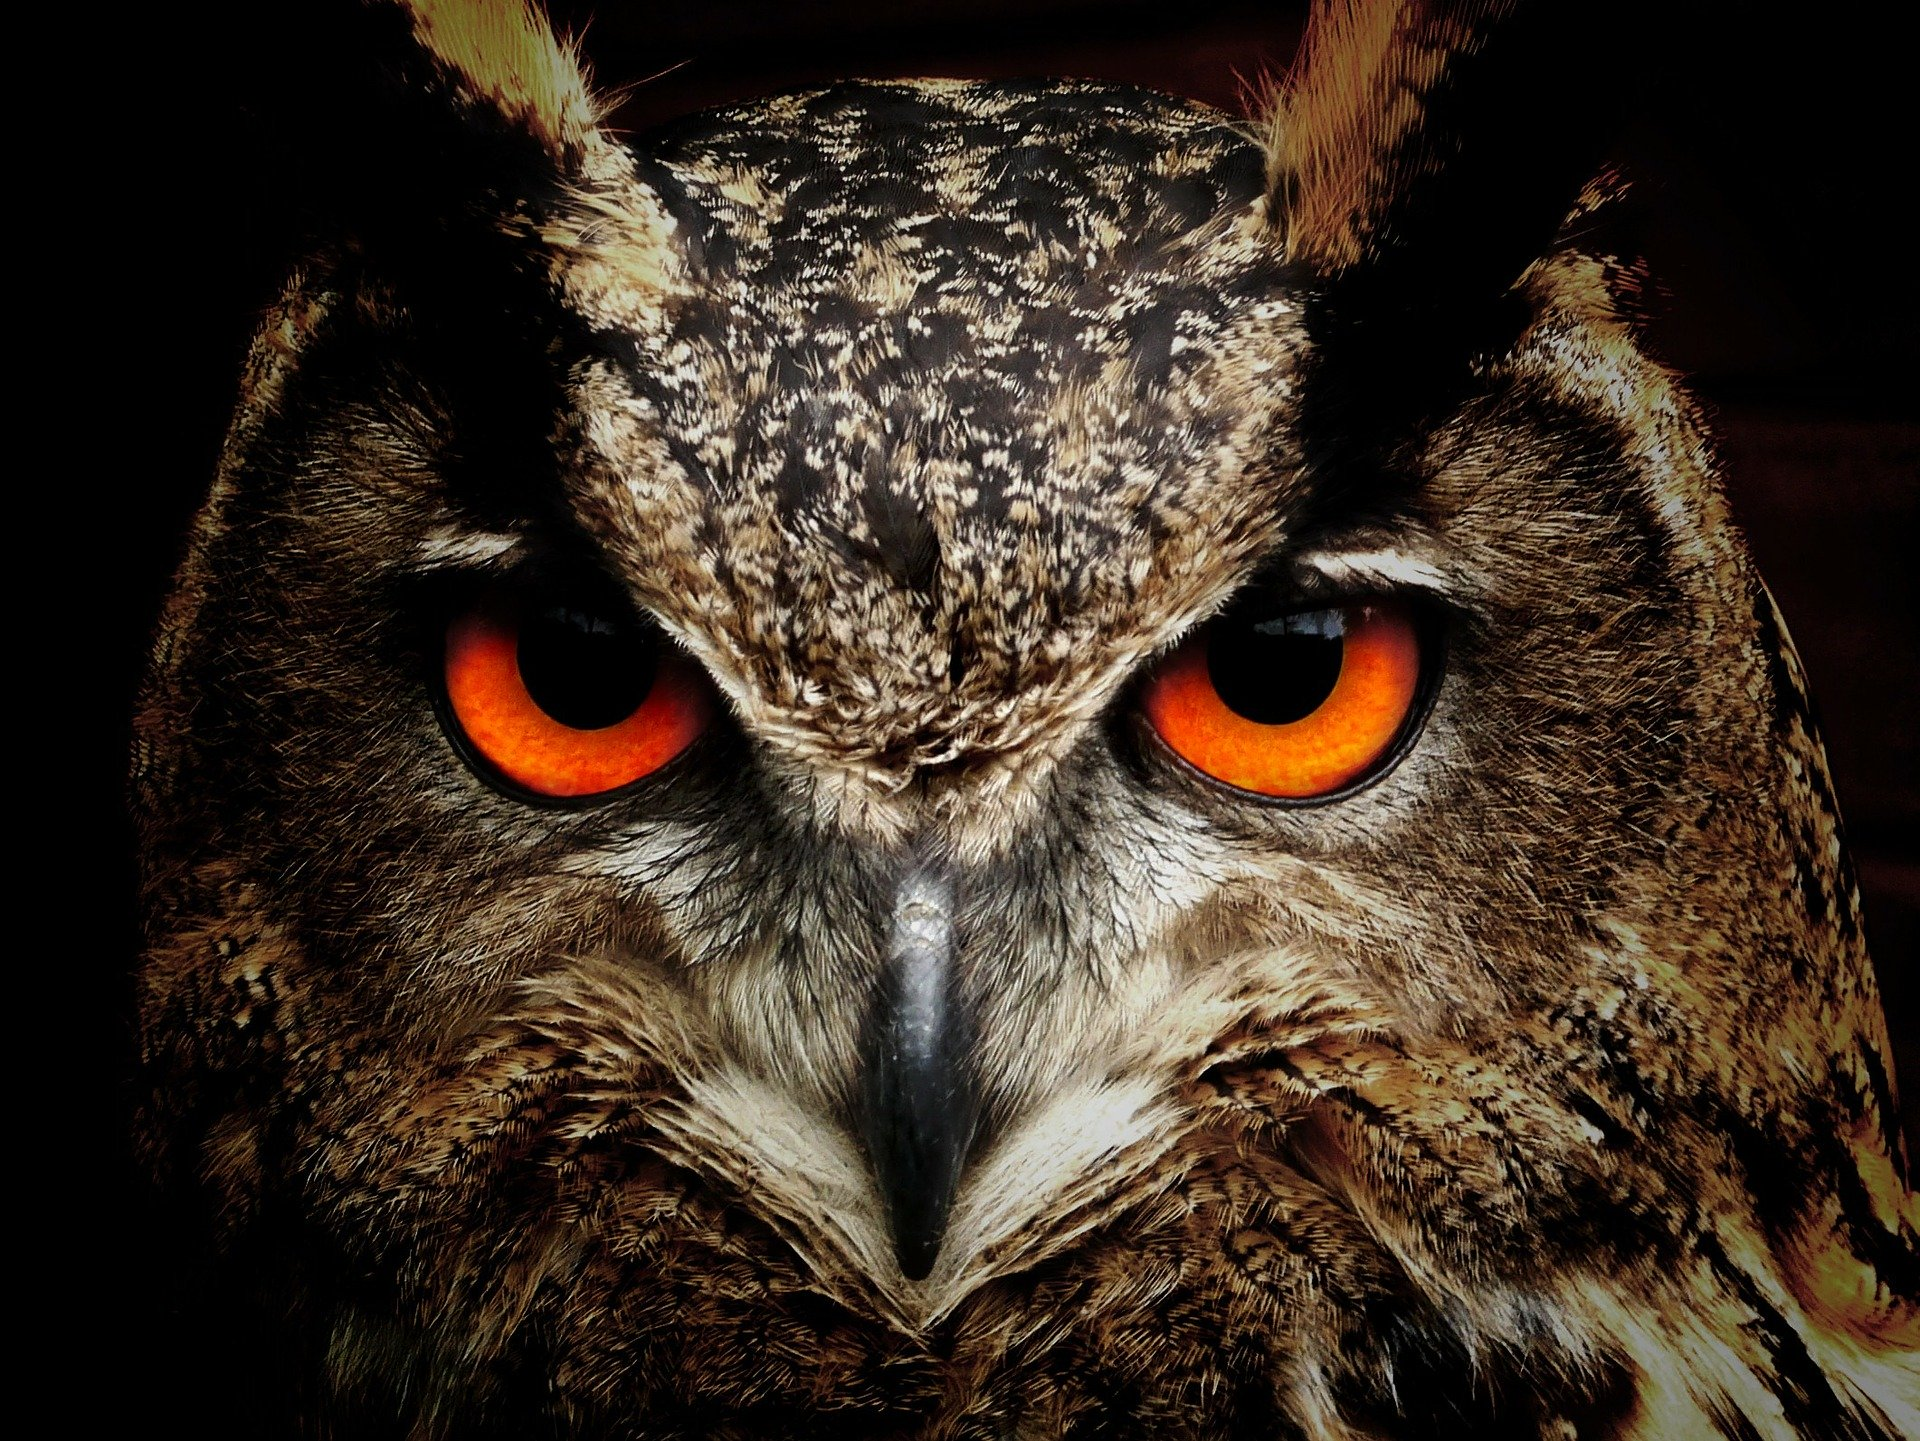
\includegraphics[scale=0.20]{../images/owl-50267_1920.jpg}

\justify
The advantages of using a revision control\index{revision control} methodology in being able to
organize and store project artifacts in a way that multiple users or
teams can leverage. Websites, like github.com for example, are
fundamental to our workflow as they are a key piece of our software
delivery pipeline.

\justify
In addition to giving us a way to back up and store our work,
essentially for free, it facilitates a greater degree of collaboration.
There are other similar, (mostly) free services we can choose from
including Bit Bucket and Git Lab. For the purposes of this book we will
focus on the most well known of these, GitHub\index{GitHub}.

\section{github.com}

Simply put, github.com is a website that allows you to store the work
you are using git to manage. Git is the tool that allows for revision
control of your work. GitHub is a repository for storing that work,
creating teams to work on projects, tracking issues, release
snapshotting, and more.

\subsection{Enable Two-Factor Authentication}

\justify
One of the very first things you should do (after creating an account,
that is) is to configure two-factor authentication\footnote{\url{https://help.github.com/en/github/authenticating-to-github/securing-your-account-with-two-factor-authentication-2fa}}
(2FA) for your GitHub account.

single: two-factor authentication

\subsection{SSH Key Setup}

Take a few minutes to generate an SSH key\index{SSH keys} pair if you don't already have
one. We will be using it at various stages to log in to various sites
and hosts. The directions for generating an SSH keypair found on the
github.com website\footnote{\url{https://help.github.com/en/github/authenticating-to-github/generating-a-new-ssh-key-and-adding-it-to-the-ssh-agent}}
are perfect for this task.

\begin{mybox}{\thetcbcounter: SSH Key Generation}
      ssh-keygen -t rsa -b 4096 -C "user@example.com"\\
      Enter a file in which to save the key (/home/user/.ssh/id\_rsa): [Press enter]\\
      Enter passphrase (empty for no passphrase): [Type a passphrase]\\
      Enter same passphrase again: [Type passphrase again]
\end{mybox}

\justify
Now you can add your public key half to github.com\footnote{\url{https://help.github.com/en/github/authenticating-to-github/adding-a-new-ssh-key-to-your-github-account}}.

\subsection{GPG Key Setup}

\justify
Using a GPG key to sign your commits\footnote{\url{https://help.github.com/en/github/authenticating-to-github/generating-a-new-gpg-key}}
will help others verify that work you check in to revision control did
actually come from you. It's not strictly necessary but is considered
good practice. Some repositories require that you sign your pull
requests with your GPG key\index{GPG key}.

\justify
Take a few minutes to set up a GPG key and add it to your profile on
GitHub.

\begin{mybox}{\thetcbcounter: GPG Key Setup}
      user@devsecops:\~\# gpg --default-new-key-algo rsa4096 --gen-key\\
      public and secret key created and signed.\\
      Note that this key cannot be used for encryption.  You may want to use
      the command "--edit-key" to generate a subkey for this purpose.\\
      pub   rsa4096 2020-05-12 [SC] [expires: 2022-05-12]\\
      \hspace*{15mm}      848943CDCE488F138BF91079E81498874E59648D\\
      uid\\
      \hspace*{25mm}                     Kevin Flynn <user@example.com>\\

      user@devsecops:\~\# gpg --list-secret-keys --keyid-format LONG |grep sec| cut -f2 -d'/'|cut -f1 -d' '\\
      E81498874E59648D\\
      user@devsecops:\~\# gpg --armor --export E81498874E59648D
\end{mybox}

Copy your GPG key, beginning with
-\/-\/-\/-\/-BEGIN PGP PUBLIC KEY BLOCK-\/-\/-\/-\/- and ending with
-\/-\/-\/-\/-END PGP PUBLIC KEY BLOCK-\/-\/-\/-\/-. Add the GPG key to
your GitHub account.

Next let's take a look at two of the key methods of interacting with
projects and other people on github.com.

\subsection{Forking and Cloning Repositories}

When someone else has a project on github.com that you would like to make changes to, you can make a "fork" of that project. Forking\index{forking} a repository means you are making a copy of that repository to your personal account on the GitHub web site.

Creating a "clone"\index{cloning a repo} of your fork to your local machine is done so that
you can make changes without altering the original project before testing and review of the changes takes place.

Adding a "remote" is a git convention to easily push changes from your clone back to the original source repository.

\begin{figure}[!htb]
      
\begin{tikzpicture}[>=latex,line join=bevel,]
  \pgfsetlinewidth{1bp}
%%
\pgfsetcolor{black}
  % Edge: orig -> fork
  \draw [->] (178.26bp,143.83bp) .. controls (169.13bp,135.07bp) and (158.04bp,124.42bp)  .. (140.85bp,107.91bp);
  % Edge: fork -> clone
  \draw [->] (140.73bp,72.202bp) .. controls (150.06bp,63.242bp) and (161.52bp,52.241bp)  .. (179.12bp,35.345bp);
  % Edge: clone -> orig
  \draw [->] (222.15bp,34.664bp) .. controls (233.94bp,44.073bp) and (246.8bp,56.959bp)  .. (253.19bp,72.0bp) .. controls (259.45bp,86.726bp) and (259.45bp,93.274bp)  .. (253.19bp,108.0bp) .. controls (248.45bp,119.15bp) and (240.16bp,129.12bp)  .. (223.62bp,144.15bp);
  % Node: orig
\begin{scope}
  \definecolor{strokecol}{rgb}{0.0,0.0,0.0};
  \pgfsetstrokecolor{strokecol}
  \draw (197.19bp,162.0bp) ellipse (168.97bp and 18.0bp);
  \draw (197.19bp,162.0bp) node {Original Repository on github.com};
\end{scope}
  % Node: fork
\begin{scope}
  \definecolor{strokecol}{rgb}{0.0,0.0,0.0};
  \pgfsetstrokecolor{strokecol}
  \draw (122.19bp,90.0bp) ellipse (122.38bp and 18.0bp);
  \draw (122.19bp,90.0bp) node {Your fork on github.com};
\end{scope}
  % Node: clone
\begin{scope}
  \definecolor{strokecol}{rgb}{0.0,0.0,0.0};
  \pgfsetstrokecolor{strokecol}
  \draw (197.19bp,18.0bp) ellipse (64.19bp and 18.0bp);
  \draw (197.19bp,18.0bp) node {Local Clone};
\end{scope}
%
\end{tikzpicture}


      \caption{Forking and cloning.}
\end{figure}

This can be a tricky pattern to master, but it is fundamental if you
want to join the ranks of Open Source contributors and developers that
enjoy the full power of Git and GitHub.


\paragraph{Steps:}

\begin{itemize}

      \item
            From the original project page on github.com, click the "fork" button.

            \begin{itemize}

                  \item
                        This creates a copy of the original repository on your personal
                        GitHub page.
            \end{itemize}
      \item
            Now from your page, make a clone of that fork from github.com to your
            machine.

            \begin{description}
                  \item[- This will allow you to add, update and test code and
                        documentation without]
                        altering the original project.
            \end{description}
      \item
            On your local machine, create a "remote" connection back to the
            original repo.
\end{itemize}

To create a "remote" called upstream from your clone to the original
repo, use this example command:

\begin{mybox}{\thetcbcounter: Create Upstream Remote}
      git remote add upstream git@github.com:hotpeppersec/rapid\_secdev\_framework.git
\end{mybox}

After completing these steps you can easily submit pull requests (PRs)
back to the original project.

\hypertarget{keeping-a-clone-in-sync}{%
      \subsection{Keeping a Clone in Sync}\label{keeping-a-clone-in-sync}}

The process of performing a pull request (PR) and merging changes is
covered fairly extensively on the Web. Let's take a quick look at how to
keep your local clone of a repository, as well as your clone on
github.com, up to date.

\hypertarget{steps-1}{%
      \paragraph{Steps}\label{steps-1}}

These are the steps to take once your pull request is merged to the main
branch in the main project repository. From the command line on the
machine where your clone resides:

\begin{itemize}
      \item
            git checkout master
      \item
            git fetch upstream
      \item
            git rebase upstream/master
      \item
            git push origin master
\end{itemize}


\subsection{Creating Repositories}

\justify
If you are starting out on a new project, simply creating a repo is
probably enough. Often I will start a repository on my personal account
while I use the steps in this book to get the project of fthe ground.
Later I will move the repository into an organization where the
responsibility for ownership and administration can be shared with other
folks.

\justify
While the repository is owned by me, I use a much simpler process for
managing my code check-ins.

\hypertarget{steps-2}{%
      \paragraph{Steps}\label{steps-2}}

\begin{itemize}

      \item
            Create the repository on github.com from my personal account.
      \item
            Make a clone of that new repository from github.com to my local host.
      \item
            Do my pull requests and merges as desired.
      \item
            Do a git pull to my master branch to keep my local clone up to date.
\end{itemize}


\subsection{Example Repository}

\justify
A GitHub Template Repository is available should you decide to follow
along with the code examples in this book. The next sets of steps are
predicated on having Docker installed and running as described in the
previous chapter.


\paragraph{Template Steps}

\begin{itemize}

      \item
            Navigate to
            \url{https://github.com/hotpeppersec/rapid_secdev_framework}
      \item
            Click the green button "Use this template"
      \item
            Select a "Repository name", like "rapid\_secdev\_framework" for
            example.
      \item
            Now click "Create repository from template"
\end{itemize}

\justify
Now you have a repository in your GitHub account that you can use for
testing and completing lab examples detailed in this book. For our first
exercise, let's try to make a clone of the repository we generated from
template.


\paragraph{Cloning Steps}

\begin{itemize}
      \item
            Navigate to the main page for our new repository on github.com.
      \item
            \begin{description}
                  \item[Clone the repository to your local host by clicking on the green
                        "Clone or download" button.]
                        \begin{itemize}

                              \item
                                    Be sure to clone with "SSH" and not "HTTPS".
                        \end{itemize}
            \end{description}
      \item
            Change to the clone directory with the "cd" command.
\end{itemize}

From the rapid\_secdev\_framework directory, execute the command
make docker to get to a command prompt within the container.

Consider the following example. Notice that the command prompt changes
to indicate that you have a BASH shell in the running container.

\begin{mybox}{\thetcbcounter: Output from make docker command}
      user@devsecops:\~/rapid\_secdev\_framework\$ make docker\\
      Building test env with docker-compose\\
      docker-compose -f docker/docker-compose.yml build devsecops\\
      Building devsecops\\
      Step 1/3 : FROM python:3.9-buster\\
      ---> 4f7cd4269fa9\\
      Step 2/3 : WORKDIR /home/secdevops\\
      ---> Using cache\\
      ---> 95dc84398bc2\\
      Step 3/3 : RUN apt update; apt install -y apt-utils\\
      ---> Using cache\\
      ---> 83ea11278488\\
      Successfully built 83ea11278488\\
      Successfully tagged docker\_devsecops:latest\\
      user@devsecops:/home/secdevops\#
\end{mybox}


\subsection{CODEOWNERS}

\justify
Creating a CODEOWNERS\index{CODEOWNERS} file\footnote{\url{https://help.github.com/en/github/creating-cloning-and-archiving-repositories/about-code-owners}}
is a good way to automatically tag folks in PRs to make them aware of
changes to certain files or folders in your projects.

\justify
In it's most basic form, the CODEOWNERS file in the .github directory
simply lists the file(s) and the owner(s) on a line together.

\justify
Consider this example where we add the @hotpeppersec to the CODEOWNERS
file.

\begin{mybox}{\thetcbcounter: Adding a user to CODEOWNERS file}
      user@devsecops:/home/secdevops\# if [ ! -d ".github" ];then mkdir .github; fi\\
      user@devsecops:/home/secdevops\# echo "* @githubusername">> .github/CODEOWNERS
\end{mybox}

In this example, the @githubusername user will be tagged as a reviewer
in all pull requests.


\subsection{The .gitignore file}
\justify
Use this file\index{.gitignore} to designate items that should be excluded from revision
control. This is useful for helping keep credentials and other secrets
out of the GitHub repository.

\justify
Consider the following example .gitignore file. This will prevent you
from checking in the .DS-Store that Macintosh creates in many folders.

\begin{mybox}{\thetcbcounter: Example .gitignore file}
      root@cloudlab:\~/workspace/cloudlab\# echo ".DS\_Store" > .gitignore
\end{mybox}

\subsection{Working with Branches}

Naming your branches something useful is helpful (self documenting).

Let's look at how to create a branch

\hypertarget{steps-3}{%
      \paragraph{Steps}\label{steps-3}}


\subsection{Pull Requests}

\justify
When you make changes on a local branch, say on your personal laptop,
you will eventually want those changes to flow back into the main
project. Opening a pull request\index{Pull Request} is a means of letting other people know
you've got a set of changes ready for review and potential
changes\footnote{\url{https://help.github.com/en/github/collaborating-with-issues-and-pull-requests/about-pull-requests}}.

\justify
Keeping pull requests smaller and more frequent makes it easier for your
peers to review your changes. It also means you will be less likely to
lose work.

\justify
Let's use our changes to the CODEOWNERS file to try making a change in
our clone of the repository in GitHub, then pushing that change up to
the repository.

\hypertarget{steps-4}{%
      \paragraph{Steps}\label{steps-4}}

\begin{itemize}

      \item
            Create a new branch, for example git checkout -b newbranch
      \item
            Create the .github directory if it does not exist, then the CODEOWNERS
            file in that directory.
      \item
            Use git to add the file to the commit: git add CODEOWNERS
      \item
            Commit the file with git, git commit -S -m 'add CODEOWNERS file'
      \item
            Push this commit to github.com, git push origin newbranch
      \item
            Use the github.com website to open and merge the pull request.
\end{itemize}


\subsection{Repository Settings}

\justify
When setting up a new repository in my GitHub account, I always click
the Settings tab (with the little gear icon) and then choose the
"Branches" section. The Default branch gets set to "master". Clicking
the "Add Rule" button, entering "master" for the "Branch name pattern",
and then the green "Create" button sets up master as a protected branch.
Consider the following example {myFig2}.

\begin{figure}
      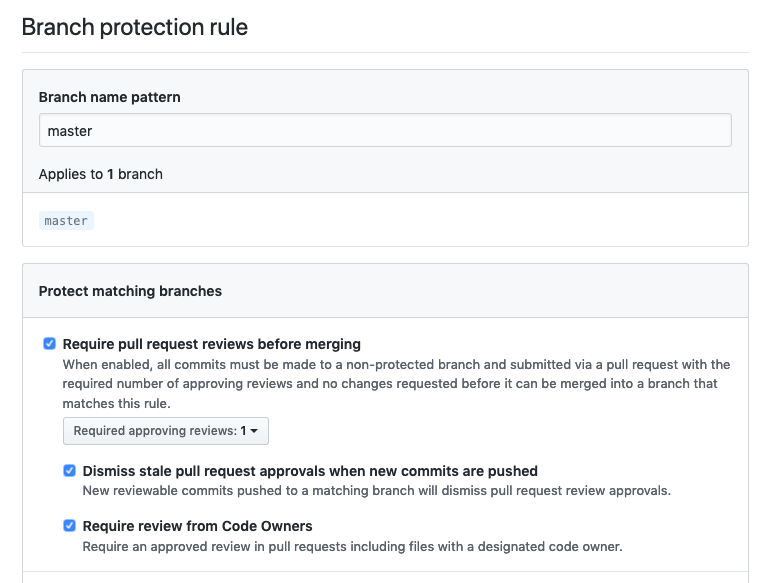
\includegraphics[scale=0.50]{../images/github-branch-protection.png}
      \caption{Setting up branch protection.}
\end{figure}

\justify
After we start to work with CI/CD tools (status checks, like GitHub
Actions for example) new choices ({myFig3}) become available in this
part of your repository for managing those checks.

\begin{figure}
      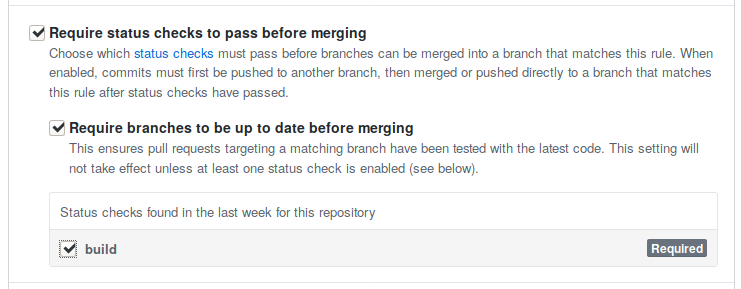
\includegraphics[scale=0.53]{../images/guthub-status-check.png}
      \caption{Requiring status checks.}
\end{figure}

\subsection{Automated Repository Scanning}

\justify
There are many GitHub plugins that are free for
single-user/non-commercial scenarios. a cursory search of the web of the
GitHub Marketplace will turn up many of these. Let's leave some of the
tedious work to the bots so we can focus on our journey to the cloud!


\subsubsection{Renovate}

WhiteSource Renovate is what's known as a dependency scanner. It is free
for single user to add from the GitHub Marketplace\footnote{\url{https://github.com/marketplace/renovate}}
. It can tell you when you are using a version of a module or image that
is out of date. For example, if you have a Dockerfile that specifies
Python 3.8.1, Renovate will open a pull request on your repository to
update the version string in that Dockerfile to the most current version
available. You can also grant Renovate the permissions required to
simply merge the change with no human interaction. Renovate supports
JavaScript, Java, Ruby, PHP, Python, Go, Cargo, Elixir, Docker, and
more.

\justify
Once you've signed up and specified which repositories you want Renovate
to monitor, it opens a pull request to install a simple default
configuration file called renovate.json. Merge this initial pull request
and you're up and running!

\subsubsection{LGTM}

Semmle is a company that runs a code scanning service we can use to keep
an eye on our repositories for issues with syntax and dependencies. It
is tightly coupled with github.com and can be configured from lgtm.com
after logging in with your GitHub credentials.

\justify
As a fun aside, LGTM stands for "looks good to me", something developers
will add as review comments when their pull request is simple or matches
obvious expectations.

\clearpage


\section{Directory Structure}

Relevant files and folders mentioned in this chapter are organized as
seen below.

\begin{figure}[!htb]
   \centering
   
\begin{tikzpicture}[>=latex,line join=bevel,]
  \pgfsetlinewidth{1bp}
%%
\pgfsetcolor{black}
  % Edge: home -> devsecops
  \draw [->] (96.5bp,215.7bp) .. controls (96.5bp,207.98bp) and (96.5bp,198.71bp)  .. (96.5bp,180.1bp);
  % Edge: devsecops -> github
  \draw [->] (85.871bp,143.7bp) .. controls (80.872bp,135.56bp) and (74.809bp,125.69bp)  .. (64.007bp,108.1bp);
  % Edge: devsecops -> gitignore
  \draw [->] (107.38bp,143.7bp) .. controls (112.49bp,135.56bp) and (118.7bp,125.69bp)  .. (129.75bp,108.1bp);
  % Edge: github -> codeowners
  \draw [->] (53.5bp,71.697bp) .. controls (53.5bp,63.983bp) and (53.5bp,54.712bp)  .. (53.5bp,36.104bp);
  % Node: home
\begin{scope}
  \definecolor{strokecol}{rgb}{0.0,0.0,0.0};
  \pgfsetstrokecolor{strokecol}
  \draw (123.5bp,252.0bp) -- (120.5bp,256.0bp) -- (99.5bp,256.0bp) -- (96.5bp,252.0bp) -- (69.5bp,252.0bp) -- (69.5bp,216.0bp) -- (123.5bp,216.0bp) -- cycle;
  \draw (96.5bp,234.0bp) node {/home};
\end{scope}
  % Node: devsecops
\begin{scope}
  \definecolor{strokecol}{rgb}{0.0,0.0,0.0};
  \pgfsetstrokecolor{strokecol}
  \draw (157.5bp,180.0bp) -- (154.5bp,184.0bp) -- (133.5bp,184.0bp) -- (130.5bp,180.0bp) -- (35.5bp,180.0bp) -- (35.5bp,144.0bp) -- (157.5bp,144.0bp) -- cycle;
  \draw (96.5bp,162.0bp) node {/home/devsecops};
\end{scope}
  % Node: github
\begin{scope}
  \definecolor{strokecol}{rgb}{0.0,0.0,0.0};
  \pgfsetstrokecolor{strokecol}
  \draw (84.0bp,108.0bp) -- (81.0bp,112.0bp) -- (60.0bp,112.0bp) -- (57.0bp,108.0bp) -- (23.0bp,108.0bp) -- (23.0bp,72.0bp) -- (84.0bp,72.0bp) -- cycle;
  \draw (53.5bp,90.0bp) node {.github};
\end{scope}
  % Node: gitignore
\begin{scope}
  \definecolor{strokecol}{rgb}{0.0,0.0,0.0};
  \pgfsetstrokecolor{strokecol}
  \draw (178.5bp,108.0bp) -- (102.5bp,108.0bp) -- (102.5bp,72.0bp) -- (178.5bp,72.0bp) -- cycle;
  \draw (140.5bp,90.0bp) node {.gitignore};
\end{scope}
  % Node: codeowners
\begin{scope}
  \definecolor{strokecol}{rgb}{0.0,0.0,0.0};
  \pgfsetstrokecolor{strokecol}
  \draw (107.0bp,36.0bp) -- (0.0bp,36.0bp) -- (0.0bp,0.0bp) -- (107.0bp,0.0bp) -- cycle;
  \draw (53.5bp,18.0bp) node {CODEOWNERS};
\end{scope}
%
\end{tikzpicture}


   \caption{GitHub related files.}
\end{figure}

\chapter{Python}

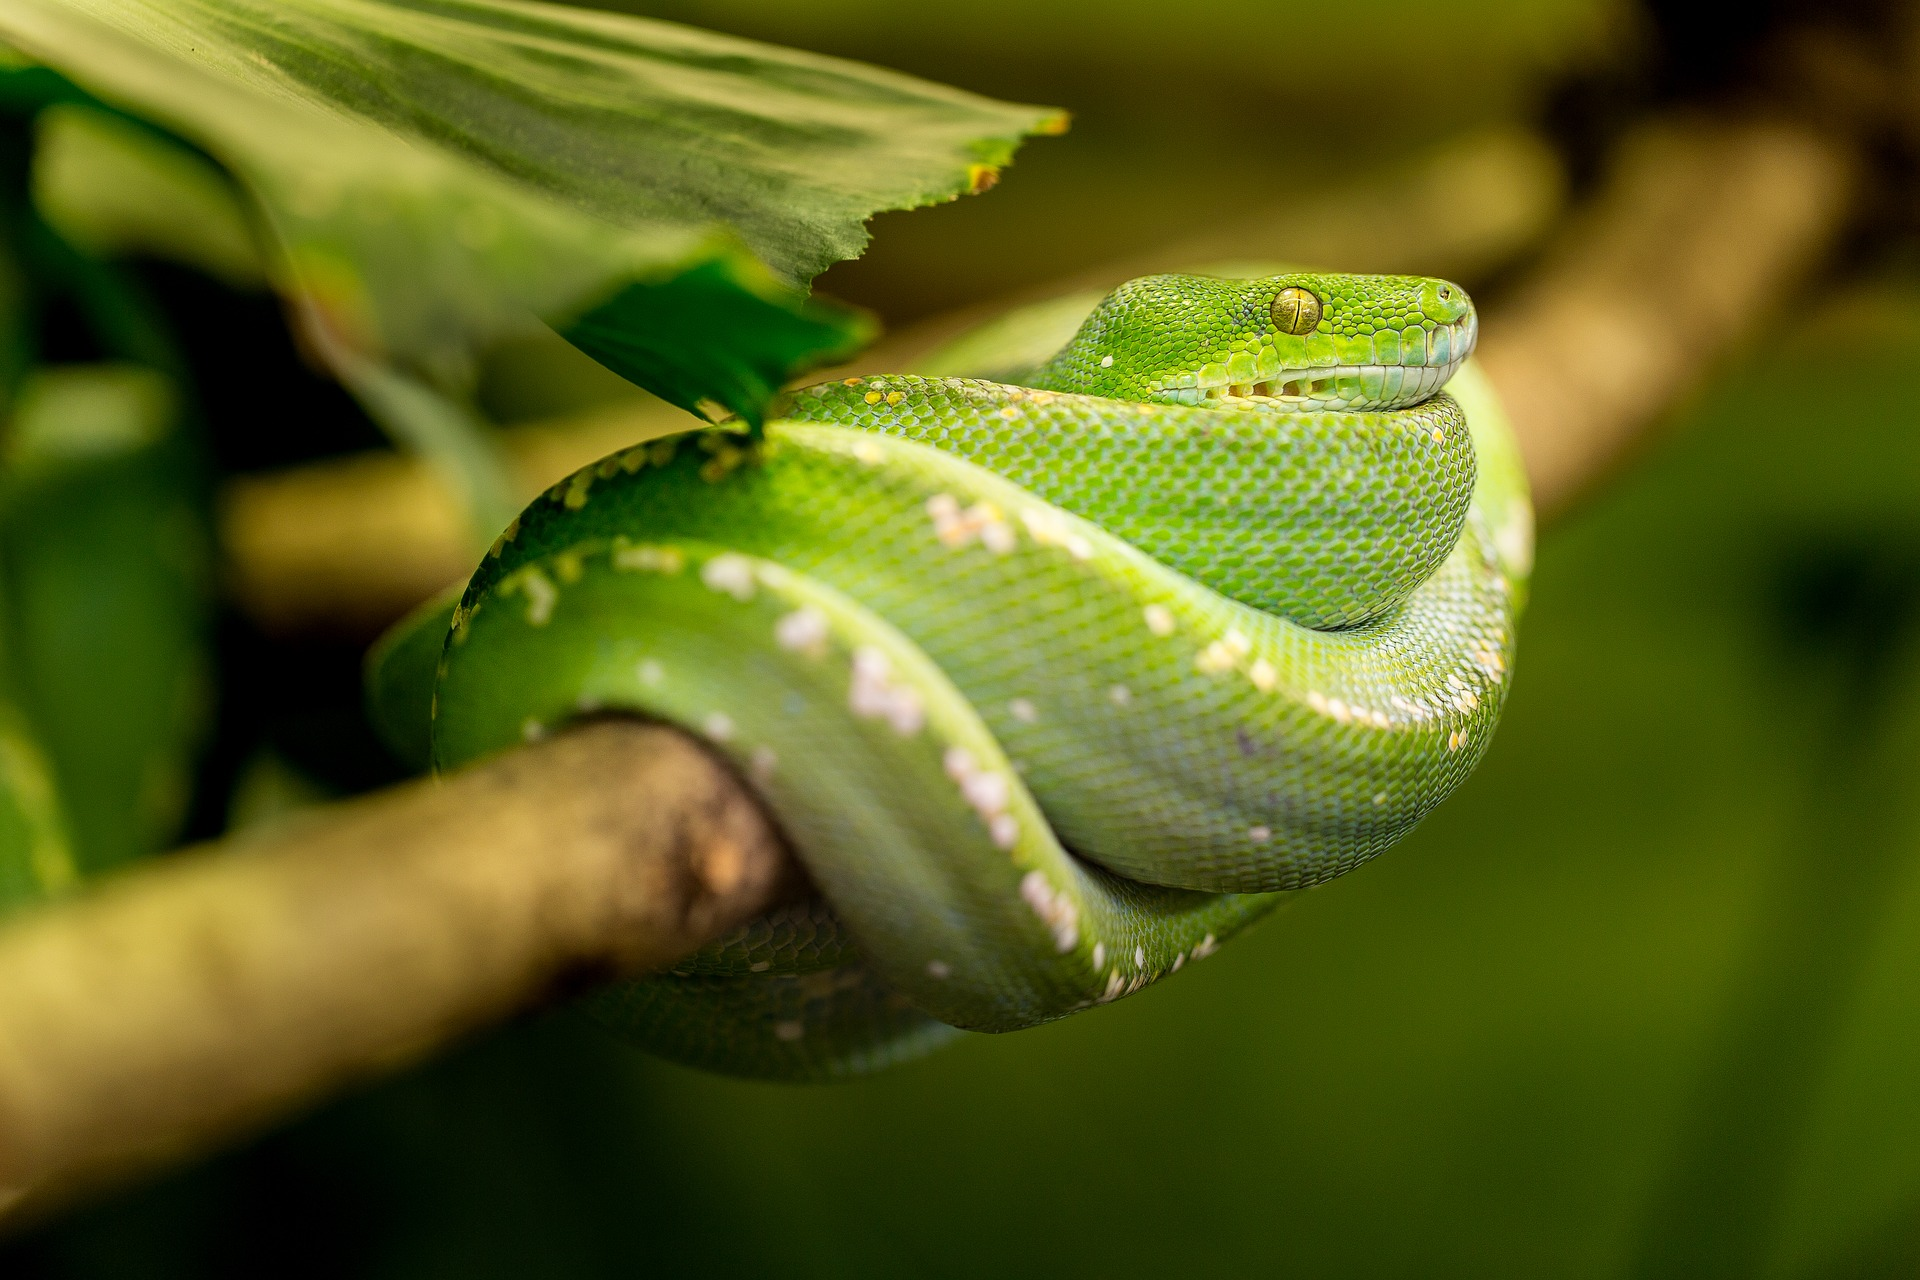
\includegraphics[scale=0.85]{../images/snake-1634293_1920.jpg}

\justify
Getting started in writing programs is easy with Python. It is highly extensible since there are many add on modules available from a collection known as Pypi\footnote{\url{https://pypi.org/}} . Python is
fairly easy to learn, especially when compared to other languages. Python runs "everywhere", for all intents and purposes. For all these reasons, Python is a great choice.

\justify
An item of note, Python3\index{Python3} is our only choice at this point. Python 2.x
End of Life was January 1st, 2020\footnote{\url{https://github.com/python/devguide/pull/344}}.


\section{The \_\_init\_\_.py File}

We add this file to let the Python interpreter know that the directories
it is found in are a contiguous part of our Python project. Since module
imports and function definitions in this file are available to all the
python code files in the directory, we can use it to our advantage. For
example, try adding this quick and dirty logging function to
python/devsecops/lib/\_\_init\_\_.py

\begin{mybox}{\thetcbcounter: python/devsecops/lib/\_\_init\_\_.py}
import logging\\
from pathlib import Path\\

Path("/var/log/devsecops").mkdir(parents=True, exist\_ok=True)\\
logging.basicConfig(\\
   filename="/var/log/devsecops/devsecops.log",\\
   level=logging.DEBUG,\\
   format="[%(asctime)s] [%(filename)s:%(lineno)s - %(funcName)5s() - %(processName)s] %(levelname)s - %(message)s"]
\end{mybox}

Now we can create a Python file log\_test.py and call the logger from
within like so:

\begin{mybox}{\thetcbcounter: log\_test.py}
import logging\\
from pathlib import Path\\

def main():\\
   logging.debug('Loggy Loggerton')\\
   if \_\_name\_\_=="\_\_main\_\_":\\
   main()
\end{mybox}

Check the results in the file /var/log/devsecops/devsecops.log.

\section{Requirements File}

\justify
A requirements file under python/requirements.txt\index{requirements.txt} lists the required
Python modules needed to build and run any Python portions of our
cloudlab project. We also add a check in the Makefile to verify the
existence of the requirements.txt file. The intention is, so we can
quickly cut and paste the Makefile into a new project, but not break
anything if no requirements are present yet.

\section{Test requirements}

\justify
Some requirements are strictly intended to be part of the test harness,
but are not needed for the application proper. Using a separate file,
such as python/requirements-test.txt\index{requirements-test.txt}, makes this delineation clear to
folks who are not familiar with the project.

\justify
Note that we can also include test requirements in our tox.ini file, as detailed in the next section.

\section{Project Testing}

Security and reliability in our lab and rapid prototyping work is just as important as it is in our work for the Production environment. In fact, you might say it's even more important since today's rapid mock ups
can easily wind up making it into the build pipeline when folks are under a time crunch to deliver.

There are many test frameworks out there, lots of great ideas put forth by the community. For our current efforts, we've settled on Tox\index{Tox} as the framework of choice. It dovetails nicely with the rest of our patterns. Tox allows us to manage requirements for virtual environments when testing, acts as a front end to pytest and coverage modules, and much more. It is highly configurable and extensible. For example we can test
that an application is compatible with multiple versions of Python.

\justify
Use the make test command inside the docker container to run the test suite for the project.

\justify
An example tox.ini\index{tox.ini} file follow. Take notice of the "deps" section, where
Python module requirements can be specified. In our current configuration, these are in lieu of test harness requirements specified in our python/requirements-test.txt file.

\begin{mybox}{\thetcbcounter: An example tox.ini file}
[tox]\\
envlist = py38
skip\_missing\_interpreters = true\\

[testenv]\\
setenv =\\
  PYTHONPATH = .\\
  PYTHONHTTPSVERIFY=0\\
deps =\\
  coverage\\
  pytest\\
commands =\\
  coverage run -m pytest -v --capture=sys\\
  coverage report --omit="*/test*,.tox/*"
\end{mybox}

\section{Test Cases}

\justify
Unit and functional testing is foundational in developing robust, secure
code. We want to be sure that when we create new code, we are also
adding test cases to our test suite that fully cover the new classes,
functions, and so on.

single: Test Cases (Python)

\justify
Consider the following example unit test case. The purpose is to test
that the function check\_docker() in the file python/cloudlab/lib/helper\_functions.py returns True when called from inside a Docker container.

\begin{mybox}{\thetcbcounter: An example Unit test case}
import pytest
from cloudlab.lib.helper\_functions import check\_docker


def test\_check\_docker():\\
   assert(check\_docker())\\
\end{mybox}

\hypertarget{test-coverage}{%
\section{Test Coverage}\label{test-coverage}}

As mentioned previously, we can avail ourselves of the coverage module
by adding it to test-requirements.txt or the deps section of our tox.ini
file. The purpose is to automatically generate a report on how much of
our code is "covered" by test cases in python/test.

single: Coverage single: Test Coverage

\section{Python Directory Structure}

Files and folders relevant to the Python portions of our project are
shown in the diagram below.

\begin{description}
\item[digraph folders \{]
1 {[}label="python", shape=folder{]}; 2 {[}label="devsecops",
shape=folder{]}; 3 {[}label="lib", shape=folder{]}; 4
{[}label="requirements.txt", shape=rectangle{]}; 5
{[}label="requirements-test.txt", shape=rectangle{]}; 6
{[}label="\_\_init\_\_.py", shape=rectangle{]}; 7
{[}label="\_\_init\_\_.py", shape=rectangle{]}; 8 {[}label="test",
shape=folder{]}; 9 {[}label="devsecops.py", shape=rectangle{]}; A
{[}label="\_\_init\_\_.py", shape=rectangle{]}; B
{[}label="\_\_init\_\_.py", shape=rectangle{]}; C {[}label="tox.ini",
shape=rectangle{]}; D {[}label="helper\_functions.py",
shape=rectangle{]};

1 -\textgreater{} 2; 1 -\textgreater{} 6; 2 -\textgreater{} 3; 1
-\textgreater{} 4; 1 -\textgreater{} 5; 2 -\textgreater{} 7; 1
-\textgreater{} 8; 2 -\textgreater{} 9; 8 -\textgreater{} A; 3
-\textgreater{} B; 1 -\textgreater{} C; 3 -\textgreater{} D;
\end{description}

\}

\chapter{Rapid Development Environments with Nix}

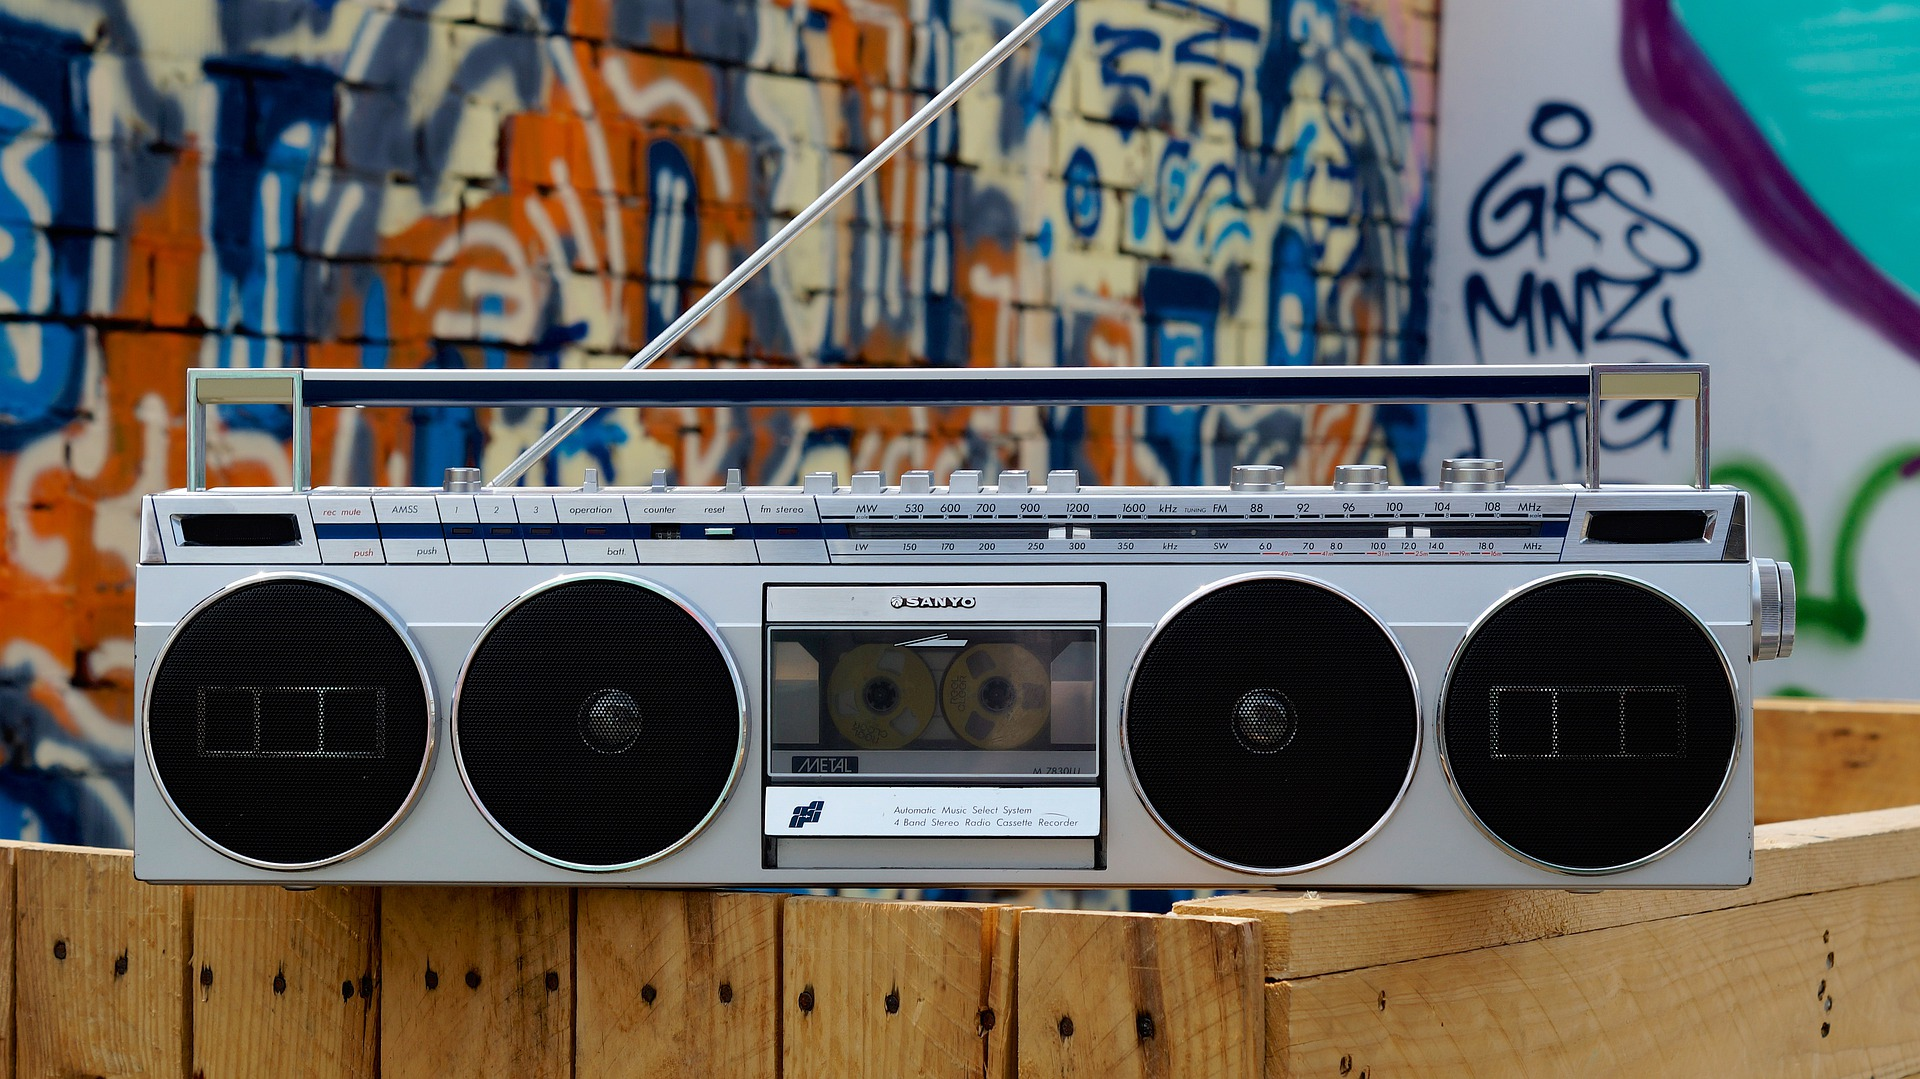
\includegraphics[scale=0.85]{images/boombox-5693150_1920.jpg}

\justify{}
Let's talk about some things.
\justify{}
Markdown Linter and Spell Check
\justify{}
Please run the linter and spell check on MD files before merging into this
repository.

\begin{mybox}{\thetcbcounter: nixlint}
    \lstinputlisting{code/nix/nix-lint.txt}
\end{mybox}

\part{Security}
\chapter{Security Concepts}

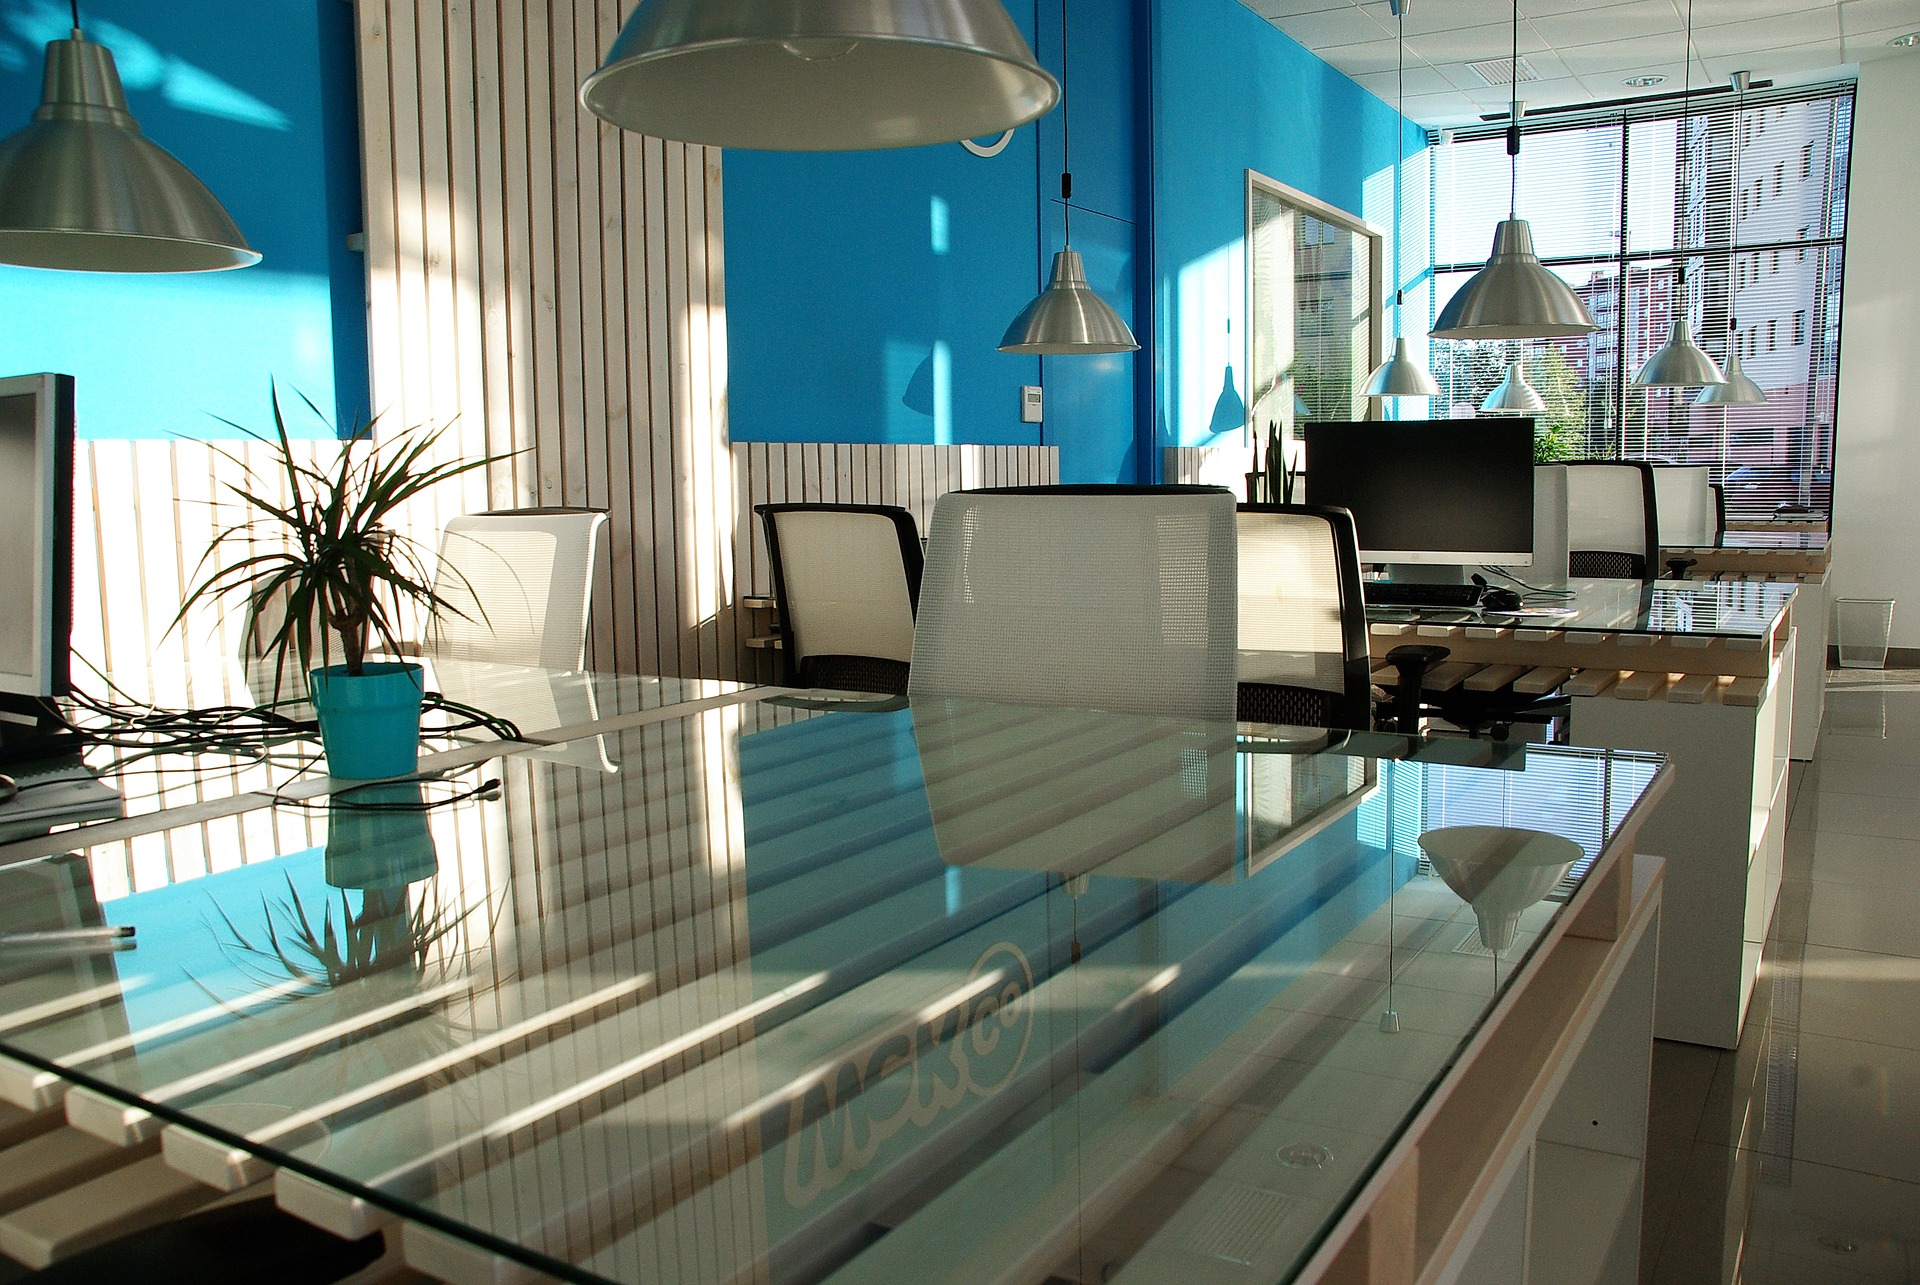
\includegraphics[scale=0.85]{images/office-space-1744803_1920.jpg}
\justify{}
Let's talk about some things.

\section{Security Mindedness}
\justify{}
This is the concept that security should be a part of all the things. 

\chapter{Security Testing}

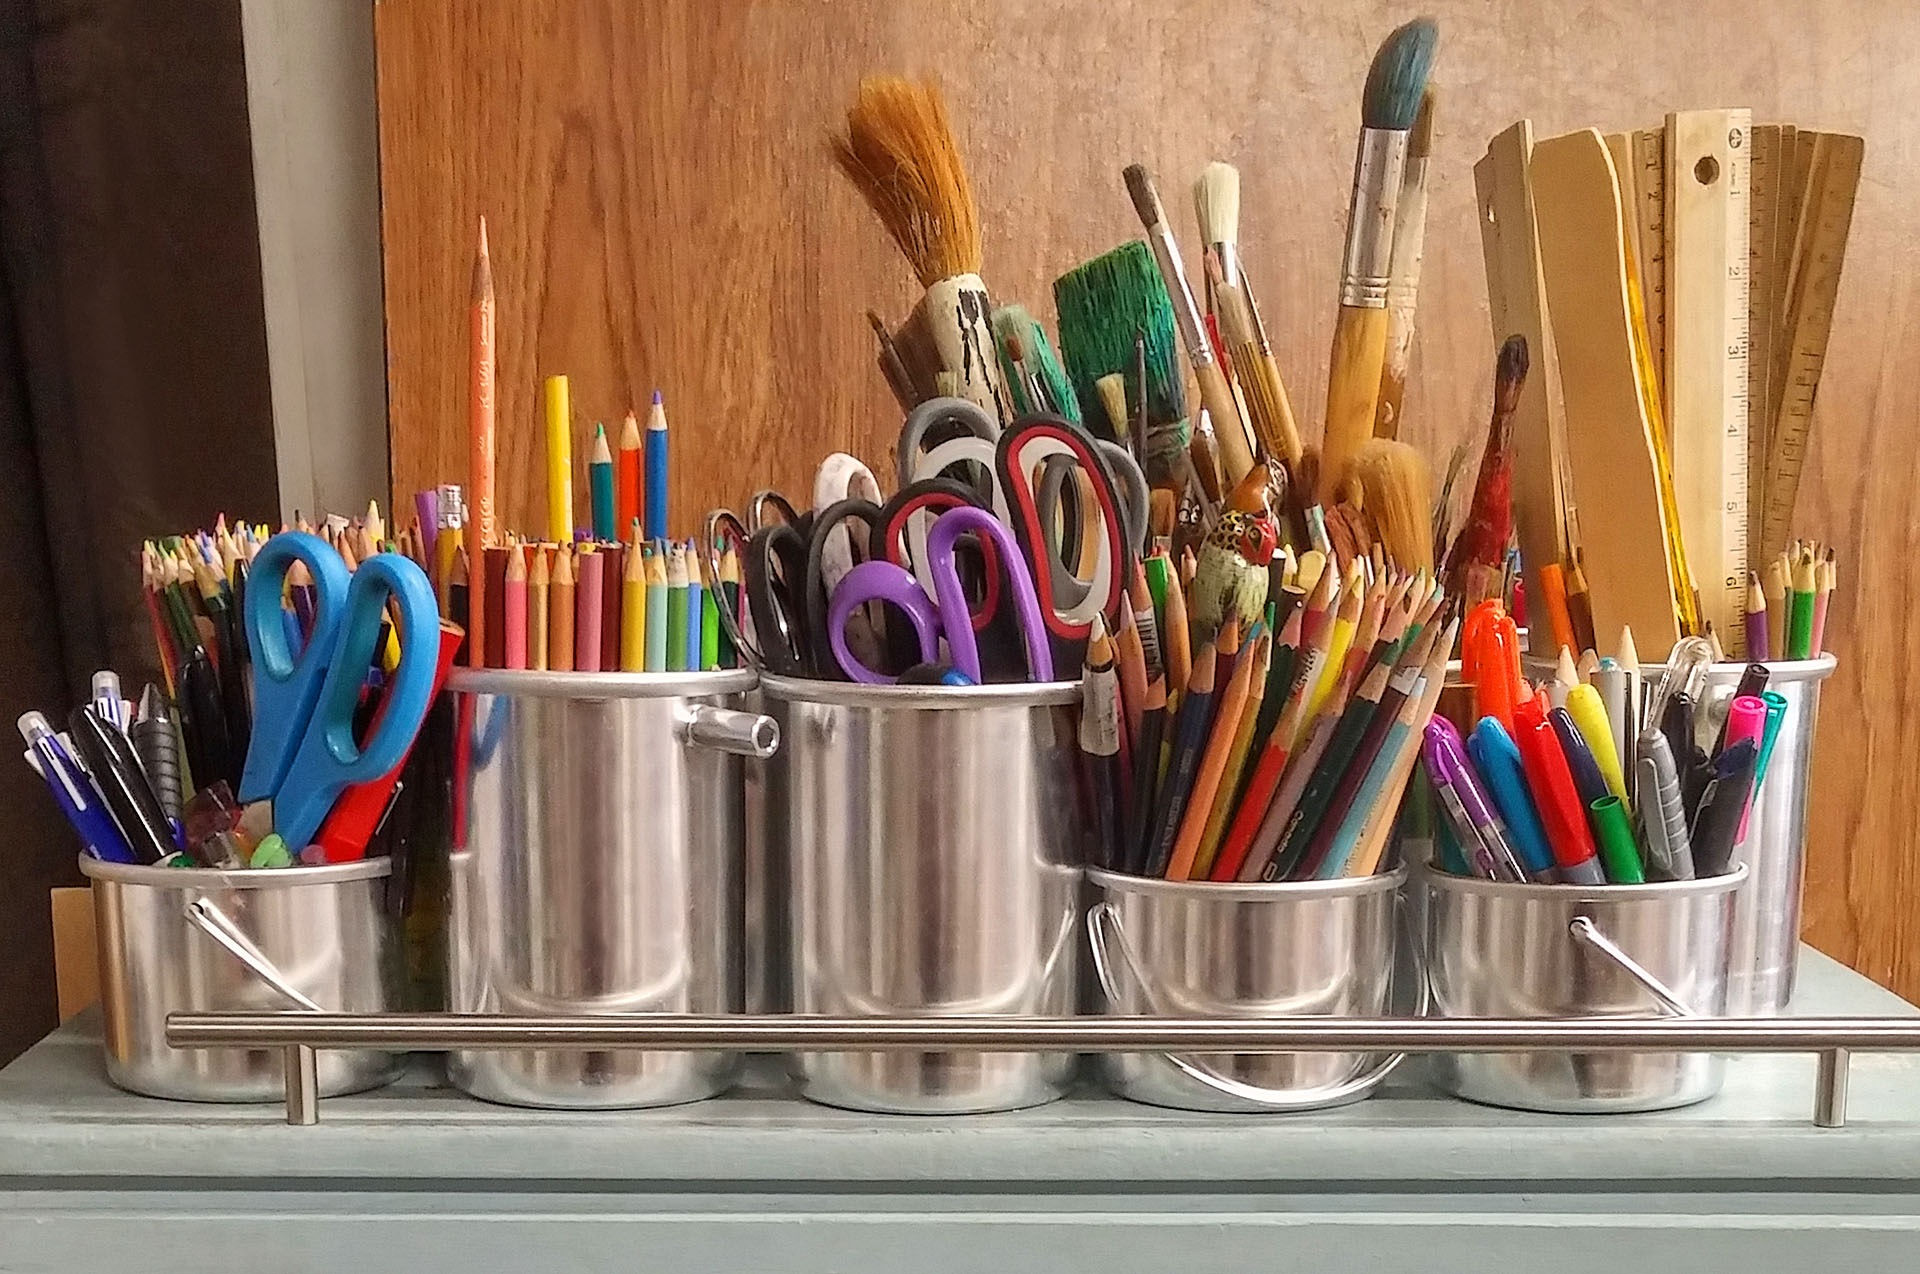
\includegraphics[scale=0.85]{../images/art-supplies-1324034.jpg}

Let's talk about some things. 

\section{SAST}
\justify{}
Talk about SAST.

\section{Policy as Code}
\justify{}
Talk about PaC.

\part{Operations}
\chapter{Makefiles}


\includegraphics[scale=0.20]{../images/books-1163695_1920.jpg}

\justify{}
A Makefile is a good way to put shorts sets of oft repeated steps at the
fingertips of the developer. Rather than typing three complicated and
possibly hard to recall strings to kick off your Docker container, you
can simply type make docker and have everything build as desired. We're
going to be using GNU Make for our projects.

\section{The PHONY Directive}

\justify{}
If a file or directory exists with the same name as a stanza in the
Makefile, you will need to specify it under the \emph{PHONY} directive.
This will allow the Makefile to find and run the desired commands.

\justify{}
Consider this example, where we have three directories (docker, docs,
and python) and we also have three Makefile directives of the same name:

\begin{mybox}{\thetcbcounter: The PHONY Directive}
	\lstinputlisting{code/07_makefiles/phony.txt}
\end{mybox}

\section{Targets}

\justify{}
Makefiles are comprised of various stanzas, know as targets. This is
where the work gets done. Let's add a target for Docker and a target for
Python to make our lives easier in the future. Consider the two target
stanzas below.

\justify{}
\begin{mybox}{\thetcbcounter: A Makefile Target}
	\lstinputlisting{code/07_makefiles/makefile-target}
\end{mybox}

\justify{}
When the user types make docker at the CLI to invoke the docker target
in the Makefile, the fist thing that happens is the python target is
called. If the file python/requirements.txt exists, we attempt to
install the modules listed within that requirements file using the
Python ``pip'' package manager. Once completed, the thread of execution
returns to the docker target. A message is sent to the user via STDOUT
that we will be building with docker-compose. An empty file at the root
of the containers filesystem named /.dockerenv is a convention that
indicates we are operating inside a containerized environment. After a
quick check for existence of the file /.dockerenv, we use docker-compose
to build from our Dockerfile, and then start a BASH shell in our
``cloudlab'' container. The user now has the ability to run BASH commands
``inside'' the Docker container.

\justify{}
Be sure when you indent in a Makefile that you use tabs, not spaces. You
can use the backslash character in a Makefile to combine two consecutive
lines into one logical line.

\section{Full Example Makefile}
\justify{}
Next, let's look at a full working example of a Makefile.

\section{Directory Structure with Makefile}
\justify{}
Relevant files and folders related to our Makefile are organized as seen
below.

\begin{figure}[!htb]
	
\begin{tikzpicture}[>=latex,line join=bevel,]
  \pgfsetlinewidth{1bp}
%%
\pgfsetcolor{black}
  % Edge: devsecops -> python
  \draw [->] (167.95bp,143.88bp) .. controls (150.51bp,134.55bp) and (128.73bp,122.92bp)  .. (101.17bp,108.19bp);
  % Edge: devsecops -> docker
  \draw [->] (188.38bp,143.7bp) .. controls (182.86bp,135.47bp) and (176.15bp,125.48bp)  .. (164.48bp,108.1bp);
  % Edge: devsecops -> terraform
  \draw [->] (211.62bp,143.7bp) .. controls (217.14bp,135.47bp) and (223.85bp,125.48bp)  .. (235.52bp,108.1bp);
  % Edge: devsecops -> Makefile
  \draw [->] (235.96bp,143.88bp) .. controls (255.88bp,134.39bp) and (280.82bp,122.51bp)  .. (311.16bp,108.07bp);
  % Edge: docker -> comp
  \draw [->] (135.2bp,71.697bp) .. controls (126.4bp,63.135bp) and (115.62bp,52.656bp)  .. (98.593bp,36.104bp);
  % Edge: docker -> Dockerfile
  \draw [->] (170.8bp,71.697bp) .. controls (179.6bp,63.135bp) and (190.38bp,52.656bp)  .. (207.41bp,36.104bp);
  % Node: devsecops
\begin{scope}
  \definecolor{strokecol}{rgb}{0.0,0.0,0.0};
  \pgfsetstrokecolor{strokecol}
  \draw (274.5bp,180.0bp) -- (271.5bp,184.0bp) -- (250.5bp,184.0bp) -- (247.5bp,180.0bp) -- (125.5bp,180.0bp) -- (125.5bp,144.0bp) -- (274.5bp,144.0bp) -- cycle;
  \draw (200.0bp,162.0bp) node {devsecops\_tactical};
\end{scope}
  % Node: python
\begin{scope}
  \definecolor{strokecol}{rgb}{0.0,0.0,0.0};
  \pgfsetstrokecolor{strokecol}
  \draw (102.0bp,108.0bp) -- (99.0bp,112.0bp) -- (78.0bp,112.0bp) -- (75.0bp,108.0bp) -- (36.0bp,108.0bp) -- (36.0bp,72.0bp) -- (102.0bp,72.0bp) -- cycle;
  \draw (69.0bp,90.0bp) node {python};
\end{scope}
  % Node: docker
\begin{scope}
  \definecolor{strokecol}{rgb}{0.0,0.0,0.0};
  \pgfsetstrokecolor{strokecol}
  \draw (185.5bp,108.0bp) -- (182.5bp,112.0bp) -- (161.5bp,112.0bp) -- (158.5bp,108.0bp) -- (120.5bp,108.0bp) -- (120.5bp,72.0bp) -- (185.5bp,72.0bp) -- cycle;
  \draw (153.0bp,90.0bp) node {docker};
\end{scope}
  % Node: terraform
\begin{scope}
  \definecolor{strokecol}{rgb}{0.0,0.0,0.0};
  \pgfsetstrokecolor{strokecol}
  \draw (290.0bp,108.0bp) -- (287.0bp,112.0bp) -- (266.0bp,112.0bp) -- (263.0bp,108.0bp) -- (204.0bp,108.0bp) -- (204.0bp,72.0bp) -- (290.0bp,72.0bp) -- cycle;
  \draw (247.0bp,90.0bp) node {terraform};
\end{scope}
  % Node: Makefile
\begin{scope}
  \definecolor{strokecol}{rgb}{0.0,0.0,0.0};
  \pgfsetstrokecolor{strokecol}
  \draw (385.5bp,108.0bp) -- (308.5bp,108.0bp) -- (308.5bp,72.0bp) -- (385.5bp,72.0bp) -- cycle;
  \draw (347.0bp,90.0bp) node {Makefile};
\end{scope}
  % Node: comp
\begin{scope}
  \definecolor{strokecol}{rgb}{0.0,0.0,0.0};
  \pgfsetstrokecolor{strokecol}
  \draw (162.0bp,36.0bp) -- (0.0bp,36.0bp) -- (0.0bp,0.0bp) -- (162.0bp,0.0bp) -- cycle;
  \draw (81.0bp,18.0bp) node {docker-compose.yml};
\end{scope}
  % Node: Dockerfile
\begin{scope}
  \definecolor{strokecol}{rgb}{0.0,0.0,0.0};
  \pgfsetstrokecolor{strokecol}
  \draw (269.5bp,36.0bp) -- (180.5bp,36.0bp) -- (180.5bp,0.0bp) -- (269.5bp,0.0bp) -- cycle;
  \draw (225.0bp,18.0bp) node {Dockerfile};
\end{scope}
%
\end{tikzpicture}


	\caption{Makefile and related files.}
\label{makefile}
\end{figure}

\chapter{Continuous Integration \& Deployment}

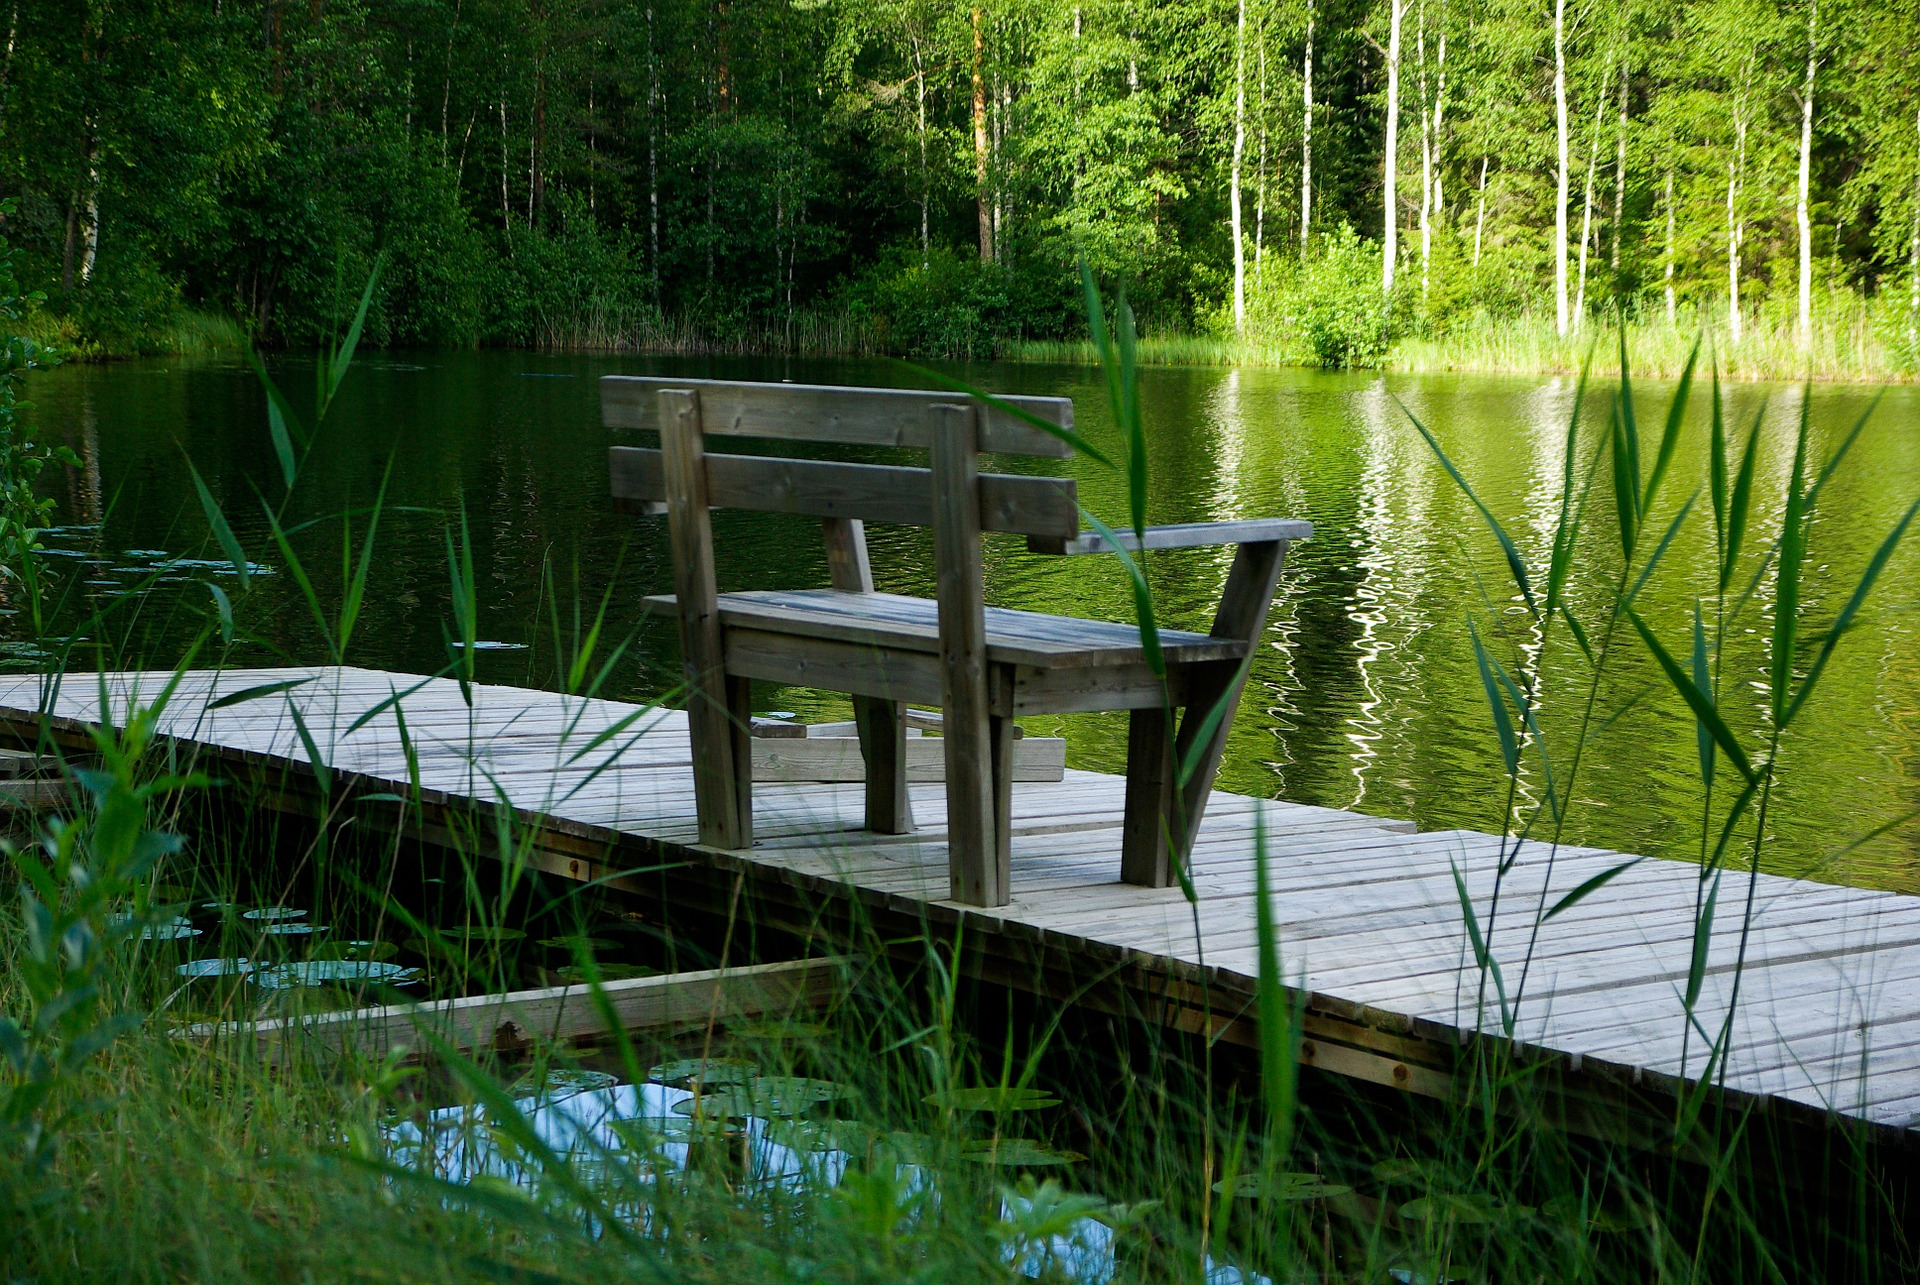
\includegraphics[scale=0.20]{../images/finland-905712_1920.jpg}

\justify
Accommodations for Continuous Integration (CI) and Continuous Deployment
(CD) in our projects directly corresponds to our chances of success.

\section{Linters}

\justify
There are small programs for most (every?) language that you can run before
pushing your changes to GitHub that will catch syntactical and sometimes
even programmatic issues. Consider Python, which is very sensitive with
regard to indentation. You can programatically detect and even correct issues
before your work gets too far down the pipe. This is also a good way to
make sure folks are not committing dirty code to your repositories.

\justify
Here are some of the linters I have found useful for languages I encounter
frequently.

%\begin{table}[h]
%	\begin{center}
%		\begin{tabular}{| p{2.5cm}| p{2.5cm} | p{2.5cm} |}
%			\hline
%			\textbf{Language} & \textbf{Name} & \textbf{Source}\hfill                                                        \\
%			Ansible           & ansible-lint  & python (pip install ansible-lint)                                      \\
%			Markdown          & mdl           & ruby (gem install mdl)                                                 \\
%			Puppet            & puppet-lint   & ruby (gem install puppet-lint)\url{http://puppet-lint.com/}} \\
%			Python            & pylint/flake8 & python (pip install pylint/flake8)                                     \\
%		\end{tabular}
%	\end{center}
%\end{table}

\subsection{Linting with Tox}

Recall that we are using Tox as our main test framework. To set up Tox
to do our linting work for us, we can add an environment to our envlist
called "pylint" and then declare it in a new stanza in tox.ini. Notice
how we let "deps" do the work of installing the "pylint" dependency for
us.

\begin{mybox}{\thetcbcounter: An Example tox.ini file}
	\lstinputlisting{code/08cicd/toxfile-pylint}
\end{mybox}

\section{GitHub Actions}

\justify
GitHub Actions is a recent introduction to the github.com website that
lets you perform Continuous Integration on your repository, and Continuous Deployment as desired.

\subsection{Docker}

Let's see how we can leverage Actions to build the docker target in our
project. Save this YAML file under
codelab/.github/workflows/docker\_compose.yml to have GitHub Actions
execute our make docker target from our custom Makefile.

%\begin{mybox}{\thetcbcounter: A Makefile Target}
%	\lstinputlisting{code/makefile-target}
%\end{mybox}


\section{Python}

Save this YAML file under codelab/.github/workflows/python.yml to have
GitHub Actions execute our make python target from our custom Makefile.

%\begin{mybox}{\thetcbcounter: Python GitHub action}
%	\lstinputlisting{code/makefile-target}
%\end{mybox}

\subsection{Packer}

Save this YAML file under devsecops\_tactical/.github/workflows/packer.yml to have
GitHub Actions validate and build our AMI image with Packer.

%\begin{mybox}{\thetcbcounter: AWS Debian host with packer}
%	\lstinputlisting{code/aws-debian-host.json}
%\end{mybox}

\subsection{Markdown}

The following example YAML file illustrates how to validate GitHub
flavored Markdown text files using a GitHub Action.

%\begin{mybox}{\thetcbcounter: A GitHub Action for linting markdown files}
%	\lstinputlisting{code/makefile-target}
%\end{mybox}

\justify
Note the designation of a configuration file named .markdownlint.json at
the top level of our repository. This JSON file is used to skip certain
checks by the markdownlint tool.

\justify
%\begin{mybox}{\thetcbcounter: The .markdownlint.json config file}
%	\lstinputlisting{code/makefile-target}
%\end{mybox}

\section{Circle CI}

Circle CI is a Continuous Integation service free for non-commercial
projects.

single: Circle CI

\justify
%\begin{mybox}{\thetcbcounter: A Circle CI configuration file}
%	\lstinputlisting{code/makefile-target} 
%\end{mybox}

\section{TravisCI}

\justify
Travis CI is a hosted continuous integration service used to build and
test software projects hosted at GitHub and Bitbucket. They have a great
tutorial available
if you care to dig a bit deeper.

\justify
By enabling Travis CI integration through the GitHub Marketplace you
can integrate their scanners with your repository.

\subsubsection{Docker}

\justify
You can test Docker containers in your CI/CD pipeline. As seen in the
following example I created a YAML file named .travis.yml to enable
automatic molecule testing of ansible roles in Travis CI. I also set a
flag in the repo settings that prevent the PR from being merged until
Travis CI flags the build as passing.

\justify
%\begin{mybox}{\thetcbcounter: A Docker container test}
%	\lstinputlisting{code/makefile-target}
%\end{mybox}

The contents of the requirements files and the example Ansible code is
available in the companion repo.


\subsection{Markdown}

Save these lines to a file named .travis.yml to scan all the markdown files in your repository.

\justify
%begin{mybox}{\thetcbcounter: A Travis config file}
%	\lstinputlisting{code/makefile-target}
%\end{mybox}

\justify
You can also create an .mdlrc file to give mdl direction on what to scan for.

\justify
%\begin{mybox}{\thetcbcounter: A Markdown lint config file}
%	\lstinputlisting{code/makefile-target}
%\end{mybox}

\clearpage

\section{Directory Structure}

\justify
Relevant folders and files related to our build pipeline are shown below. The users home directory
and workspace subdirectory is implied and removed from the diagram for clarity.

\begin{figure}[!htb]
	
\begin{tikzpicture}[>=latex,line join=bevel,]
  \pgfsetlinewidth{1bp}
%%
\pgfsetcolor{black}
  % Edge: framework -> dotgh
  \draw [->] (95.919bp,144.33bp) .. controls (117.02bp,162.13bp) and (151.1bp,189.03bp)  .. (184.0bp,207.0bp) .. controls (194.07bp,212.5bp) and (205.5bp,217.37bp)  .. (225.81bp,224.87bp);
  % Edge: framework -> dotcircleci
  \draw [->] (135.35bp,144.06bp) .. controls (160.62bp,151.61bp) and (189.41bp,160.23bp)  .. (222.3bp,170.07bp);
  % Edge: framework -> dottr
  \draw [->] (148.16bp,126.0bp) .. controls (164.99bp,126.0bp) and (182.65bp,126.0bp)  .. (208.94bp,126.0bp);
  % Edge: framework -> mdlrc
  \draw [->] (135.35bp,107.94bp) .. controls (162.44bp,99.842bp) and (193.57bp,90.528bp)  .. (227.06bp,80.507bp);
  % Edge: framework -> mdjson
  \draw [->] (95.919bp,107.67bp) .. controls (117.02bp,89.868bp) and (151.1bp,62.975bp)  .. (184.0bp,45.0bp) .. controls (187.0bp,43.36bp) and (190.12bp,41.776bp)  .. (202.43bp,36.133bp);
  % Edge: dotgh -> workflows
  \draw [->] (287.33bp,234.0bp) .. controls (306.56bp,234.0bp) and (332.12bp,234.0bp)  .. (365.0bp,234.0bp);
  % Edge: workflows -> dcy
  \draw [->] (433.91bp,252.13bp) .. controls (449.27bp,263.45bp) and (470.12bp,277.77bp)  .. (490.0bp,288.0bp) .. controls (493.26bp,289.68bp) and (496.64bp,291.3bp)  .. (509.32bp,296.86bp);
  % Edge: workflows -> py
  \draw [->] (454.2bp,241.74bp) .. controls (471.05bp,244.72bp) and (490.51bp,248.17bp)  .. (518.5bp,253.12bp);
  % Edge: workflows -> pyyml
  \draw [->] (454.2bp,226.26bp) .. controls (470.9bp,223.31bp) and (490.17bp,219.89bp)  .. (517.97bp,214.97bp);
  % Edge: workflows -> mdy
  \draw [->] (440.67bp,215.75bp) .. controls (445.18bp,212.89bp) and (449.74bp,209.91bp)  .. (454.0bp,207.0bp) .. controls (470.51bp,195.72bp) and (472.44bp,189.57bp)  .. (490.0bp,180.0bp) .. controls (493.06bp,178.33bp) and (496.24bp,176.73bp)  .. (508.79bp,171.03bp);
  % Edge: dotcircleci -> cy
  \draw [->] (290.64bp,180.0bp) .. controls (309.82bp,180.0bp) and (334.41bp,180.0bp)  .. (366.24bp,180.0bp);
  % Node: framework
\begin{scope}
  \definecolor{strokecol}{rgb}{0.0,0.0,0.0};
  \pgfsetstrokecolor{strokecol}
  \draw (148.0bp,144.0bp) -- (145.0bp,148.0bp) -- (124.0bp,148.0bp) -- (121.0bp,144.0bp) -- (0.0bp,144.0bp) -- (0.0bp,108.0bp) -- (148.0bp,108.0bp) -- cycle;
  \draw (74.0bp,126.0bp) node {devsecops\_tactical};
\end{scope}
  % Node: dotgh
\begin{scope}
  \definecolor{strokecol}{rgb}{0.0,0.0,0.0};
  \pgfsetstrokecolor{strokecol}
  \draw (287.0bp,252.0bp) -- (284.0bp,256.0bp) -- (263.0bp,256.0bp) -- (260.0bp,252.0bp) -- (226.0bp,252.0bp) -- (226.0bp,216.0bp) -- (287.0bp,216.0bp) -- cycle;
  \draw (256.5bp,234.0bp) node {.github};
\end{scope}
  % Node: dotcircleci
\begin{scope}
  \definecolor{strokecol}{rgb}{0.0,0.0,0.0};
  \pgfsetstrokecolor{strokecol}
  \draw (290.5bp,198.0bp) -- (287.5bp,202.0bp) -- (266.5bp,202.0bp) -- (263.5bp,198.0bp) -- (222.5bp,198.0bp) -- (222.5bp,162.0bp) -- (290.5bp,162.0bp) -- cycle;
  \draw (256.5bp,180.0bp) node {.circleci};
\end{scope}
  % Node: dottr
\begin{scope}
  \definecolor{strokecol}{rgb}{0.0,0.0,0.0};
  \pgfsetstrokecolor{strokecol}
  \draw (304.0bp,144.0bp) -- (209.0bp,144.0bp) -- (209.0bp,108.0bp) -- (304.0bp,108.0bp) -- cycle;
  \draw (256.5bp,126.0bp) node {.travis.yml};
\end{scope}
  % Node: mdlrc
\begin{scope}
  \definecolor{strokecol}{rgb}{0.0,0.0,0.0};
  \pgfsetstrokecolor{strokecol}
  \draw (285.5bp,90.0bp) -- (227.5bp,90.0bp) -- (227.5bp,54.0bp) -- (285.5bp,54.0bp) -- cycle;
  \draw (256.5bp,72.0bp) node {.mdlrc};
\end{scope}
  % Node: mdjson
\begin{scope}
  \definecolor{strokecol}{rgb}{0.0,0.0,0.0};
  \pgfsetstrokecolor{strokecol}
  \draw (329.0bp,36.0bp) -- (184.0bp,36.0bp) -- (184.0bp,0.0bp) -- (329.0bp,0.0bp) -- cycle;
  \draw (256.5bp,18.0bp) node {.markdownlint.json};
\end{scope}
  % Node: workflows
\begin{scope}
  \definecolor{strokecol}{rgb}{0.0,0.0,0.0};
  \pgfsetstrokecolor{strokecol}
  \draw (454.0bp,252.0bp) -- (451.0bp,256.0bp) -- (430.0bp,256.0bp) -- (427.0bp,252.0bp) -- (365.0bp,252.0bp) -- (365.0bp,216.0bp) -- (454.0bp,216.0bp) -- cycle;
  \draw (409.5bp,234.0bp) node {workflows};
\end{scope}
  % Node: dcy
\begin{scope}
  \definecolor{strokecol}{rgb}{0.0,0.0,0.0};
  \pgfsetstrokecolor{strokecol}
  \draw (638.0bp,333.0bp) -- (490.0bp,333.0bp) -- (490.0bp,297.0bp) -- (638.0bp,297.0bp) -- cycle;
  \draw (564.0bp,315.0bp) node {docker\_compose.yml};
\end{scope}
  % Node: py
\begin{scope}
  \definecolor{strokecol}{rgb}{0.0,0.0,0.0};
  \pgfsetstrokecolor{strokecol}
  \draw (609.5bp,279.0bp) -- (518.5bp,279.0bp) -- (518.5bp,243.0bp) -- (609.5bp,243.0bp) -- cycle;
  \draw (564.0bp,261.0bp) node {packer.yml};
\end{scope}
  % Node: pyyml
\begin{scope}
  \definecolor{strokecol}{rgb}{0.0,0.0,0.0};
  \pgfsetstrokecolor{strokecol}
  \draw (610.0bp,225.0bp) -- (518.0bp,225.0bp) -- (518.0bp,189.0bp) -- (610.0bp,189.0bp) -- cycle;
  \draw (564.0bp,207.0bp) node {python.yml};
\end{scope}
  % Node: mdy
\begin{scope}
  \definecolor{strokecol}{rgb}{0.0,0.0,0.0};
  \pgfsetstrokecolor{strokecol}
  \draw (619.0bp,171.0bp) -- (509.0bp,171.0bp) -- (509.0bp,135.0bp) -- (619.0bp,135.0bp) -- cycle;
  \draw (564.0bp,153.0bp) node {markdown.yml};
\end{scope}
  % Node: cy
\begin{scope}
  \definecolor{strokecol}{rgb}{0.0,0.0,0.0};
  \pgfsetstrokecolor{strokecol}
  \draw (452.5bp,198.0bp) -- (366.5bp,198.0bp) -- (366.5bp,162.0bp) -- (452.5bp,162.0bp) -- cycle;
  \draw (409.5bp,180.0bp) node {config.yml};
\end{scope}
%
\end{tikzpicture}


	\caption{CI/CD related files and folders.}
\end{figure}

\chapter{Infrastructure}

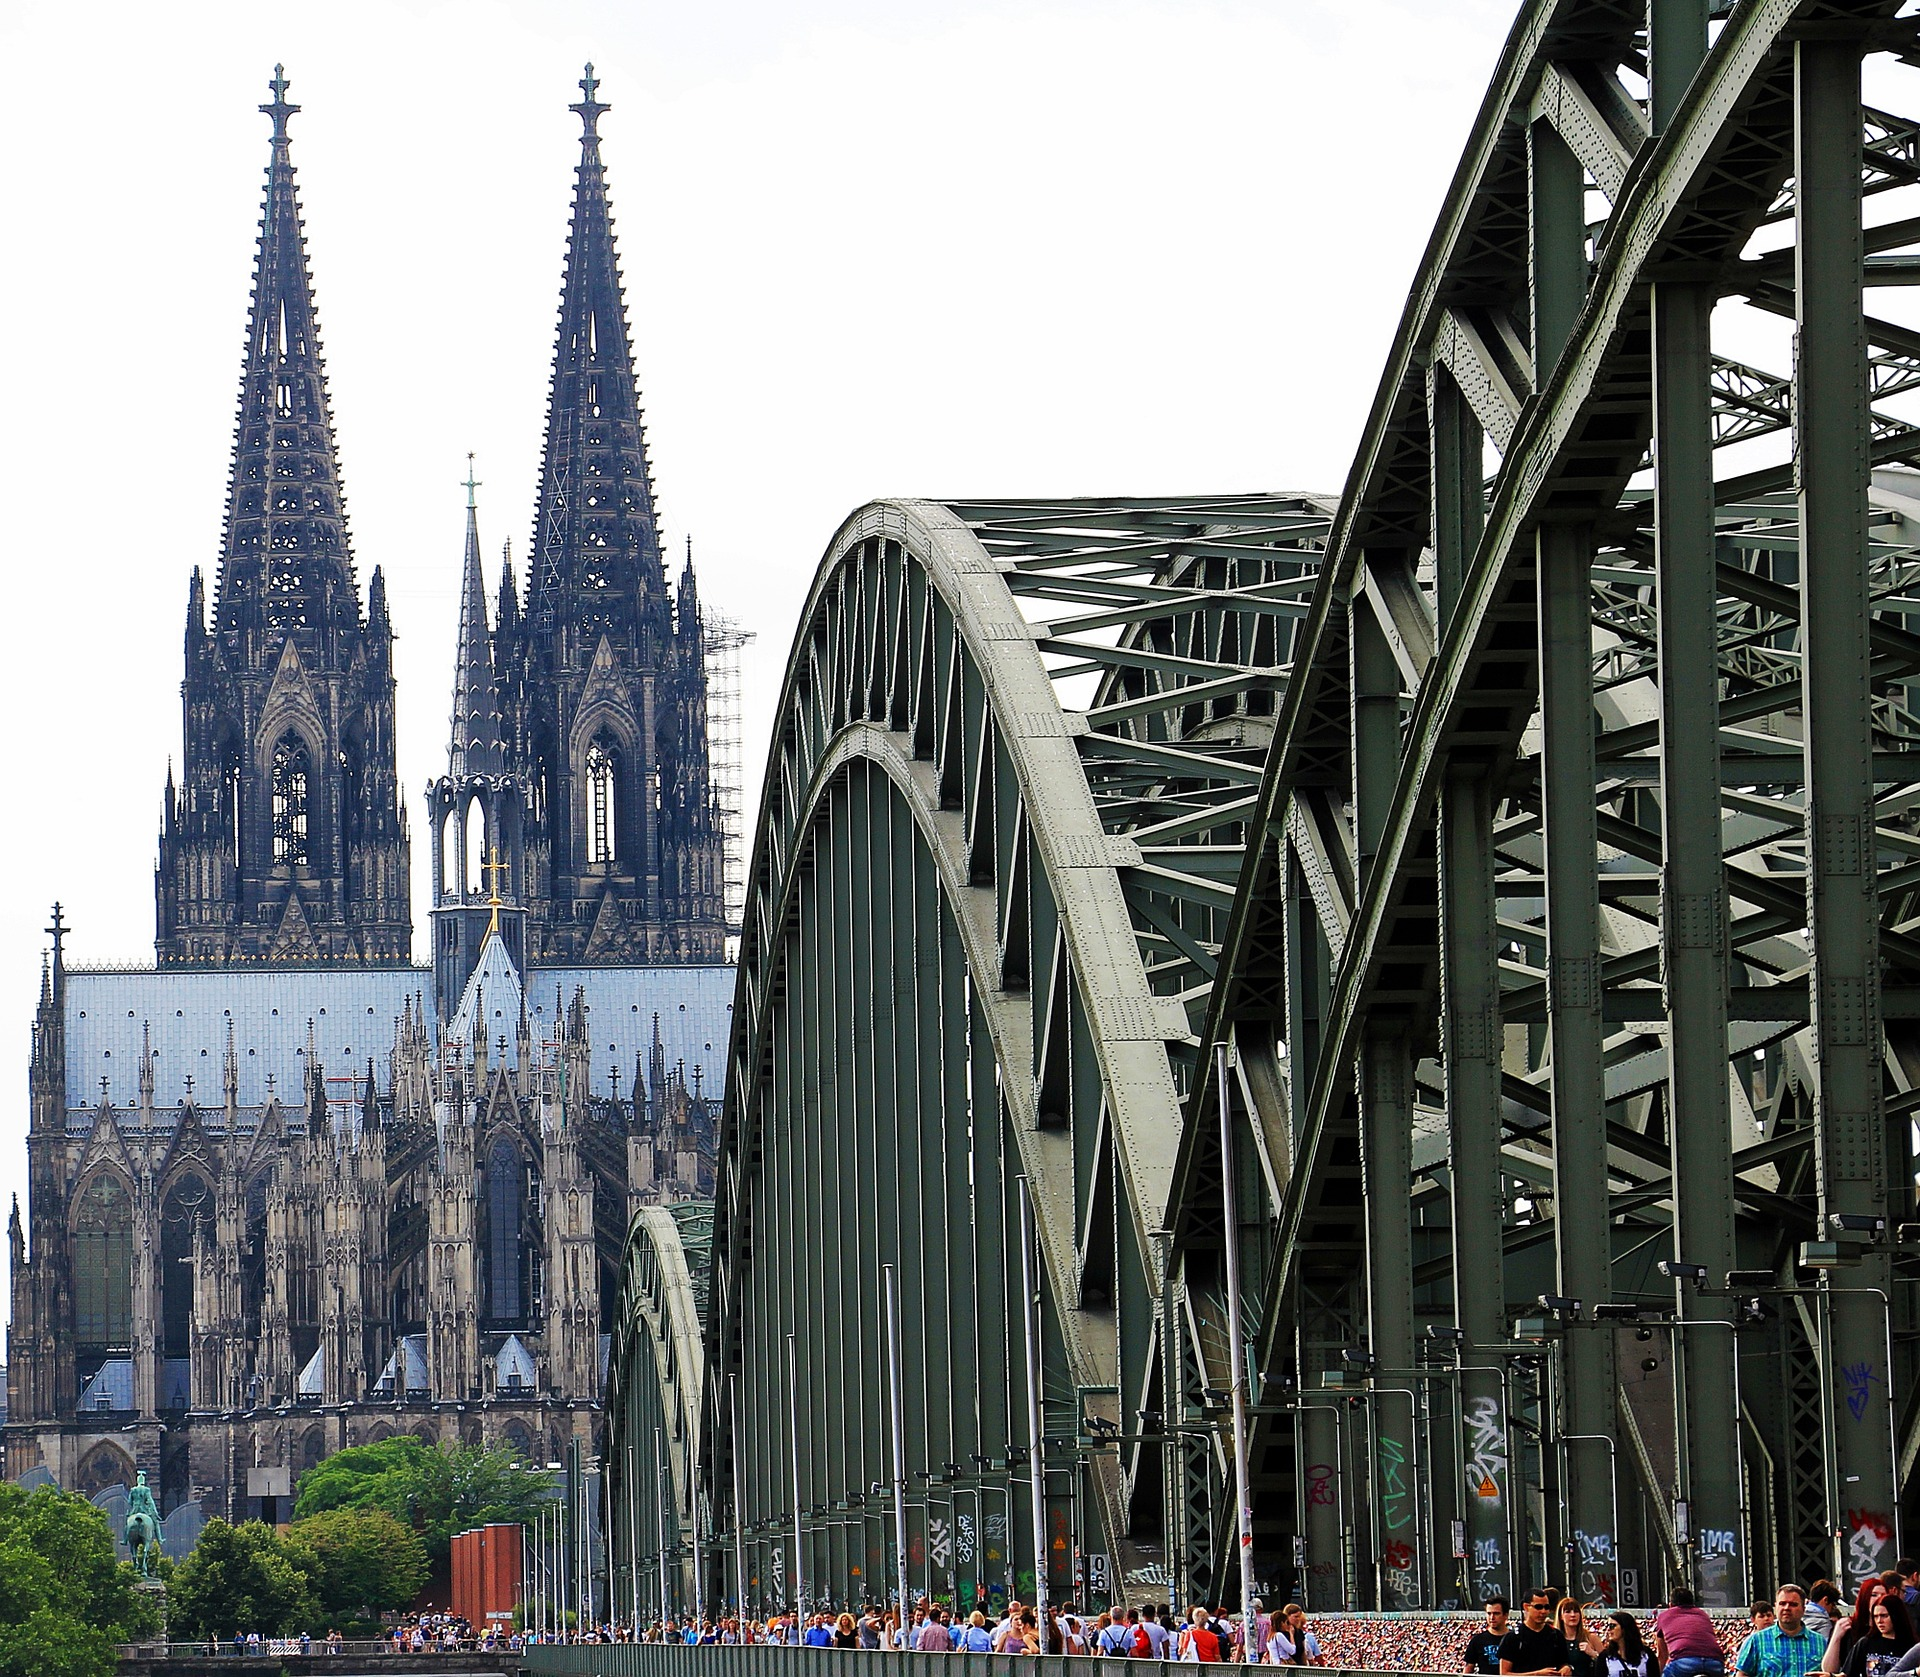
\includegraphics{../images/cologne-cathedral-1507854_1920.jpg}

\justify
Software Infrastructure and Platforms are the foundations upon which our
scripts, code, and projects are founded. Infrastructure comprises the
base upon which our containers rest, and the connectivity that allows us
to communicate with them and them with each other.

\justify
This chapter details our ability to quickly and uniformly stand up and
tear down virtual domains and networks to connect our containers and
route their workloads. We will look at some popular cloud computing
providers to prepare to explore ways we can leverage them to our
benefit.

\justify
A Cloud Provider is a company that offers to host our containerized
projects and virtual infrastructure so we don't have to do it ourselves.

single: Cloud Provider

\justify
The virtual resources we subscribe to will be distributed across cloud
provider hardware in data centers around the world with very little
oversight or interaction from us. For example, we can choose a Region of
the world for our server instance to exist in, but we don't need to
worry about which machine or rack it's in, or even where the data center
is located.

\section{Amazon Web Services (AWS)}

\justify
Consider ({myFig4}) which illustrates the connectivity of a basic
project using Amazon Web Services (AWS).

single: Amazon Web Services

\begin{figure}
  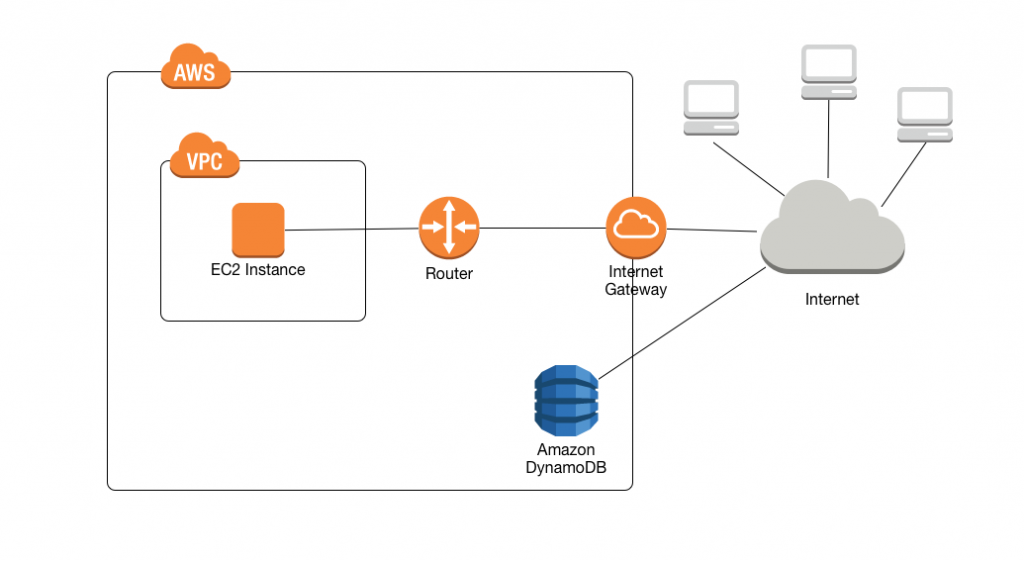
\includegraphics[scale=0.45]{../images/ddb-no-vpc-endpoint-1024x561.png}
  \caption{A simple Public Cloud configuration using AWS as a provider.}
\end{figure}

\subsection{Getting Set up in AWS}

\justify
One of the very first things you should do (after creating an account,
that is) is to configure mutli-factor authentication\footnote{MFA:
  \url{https://docs.aws.amazon.com/IAM/latest/UserGuide/id_credentials_mfa.html}}
(MFA).

single: multi-factor authentication
single: AWS single: Amazon Web Services

\justify
Amazon's AWS is one of the more prevalent cloud providers in terms of
popularity and simultaneously mature and ever-expanding feature set.

\subsection{Credentials}

\justify
Amazon Web Services (AWS) credentials are stored in a hidden directory
in your home directory called ".aws". The file
\textasciitilde{}/.aws/credentials should be modified to contain your
AWS access\_id and secret\_key as seen below.

\begin{mybox}{\thetcbcounter: ~/.aws/credentials}
  [default]\\
  aws\_access\_key\_id = AKIAJCQ6WHUXVOKZ8RQQ\\
  aws\_secret\_access\_key = q27qR8fwdHLUh7WOEH3JVd2VHjfRlQs1jlhhbZbQ\\
\end{mybox}

\justify
Do not share this file with other people. Do not check this file into
your GitHub repositories under any circumstances.

\section{Google Cloud Platform (GCP)}

\justify
Google Cloud Platform (GCP) is a suite of cloud computing services that
runs on the same infrastructure that Google uses internally for its
end-user products\footnote{\url{https://cloud.google.com/}} . If the
resources we allocate on GCP were a pyramid, the apex of that pyramid
would be a "project". A project is made up of the settings, permissions,
and other metadata that describe your applications\footnote{\url{https://cloud.google.com/docs/overview/}}.

single: Google Cloud Platform single: GCP

\justify
One of the very first things you should do (after creating an account,
that is) is to configure two-factor authentication\footnote{2FA:
  \url{https://www.google.com/landing/2step/}} (2FA).

single: two-factor authentication

\justify
At this point you are ready to install the gcloud software development
kit (SDK) on your local machine\footnote{\url{https://cloud.google.com/sdk/install}}.

single: gcloud

\subsection{Credentials}

\justify
Once the gcloud SDK is installed, you are ready to set up local
credentials that allow interaction between your machine and the GCP
application programming interface (API). In other words, Google hosts a
server that you can exchange commands with to configure your GCP
projects from your local CLI.

\justify
GCP credentials are stored in the directory
\textasciitilde{}/.config/gcloud as a JSON file. Do not share this file
with other people. Do not check this file into your GitHub repositories
under any circumstances.

\clearpage
\subsection{Directory Structure}

\justify
Relevant folders and files related to our build pipeline are shown
below. The users home directory and workspace subdirectory is implied
and removed from the diagram for clarity.

\begin{figure}[!htb]
  
\begin{tikzpicture}[>=latex,line join=bevel,]
  \pgfsetlinewidth{1bp}
%%
\pgfsetcolor{black}
  % Edge: framework -> dotcfg
  \draw [->] (168.11bp,215.7bp) .. controls (163.74bp,207.64bp) and (158.44bp,197.89bp)  .. (148.79bp,180.1bp);
  % Edge: framework -> aws
  \draw [->] (186.89bp,215.7bp) .. controls (191.26bp,207.64bp) and (196.56bp,197.89bp)  .. (206.21bp,180.1bp);
  % Edge: dotcfg -> gcloud
  \draw [->] (139.5bp,143.7bp) .. controls (139.5bp,135.98bp) and (139.5bp,126.71bp)  .. (139.5bp,108.1bp);
  % Edge: gcloud -> sdo
  \draw [->] (139.5bp,71.697bp) .. controls (139.5bp,63.983bp) and (139.5bp,54.712bp)  .. (139.5bp,36.104bp);
  % Node: framework
\begin{scope}
  \definecolor{strokecol}{rgb}{0.0,0.0,0.0};
  \pgfsetstrokecolor{strokecol}
  \draw (251.5bp,252.0bp) -- (248.5bp,256.0bp) -- (227.5bp,256.0bp) -- (224.5bp,252.0bp) -- (103.5bp,252.0bp) -- (103.5bp,216.0bp) -- (251.5bp,216.0bp) -- cycle;
  \draw (177.5bp,234.0bp) node {devsecops\_tactical};
\end{scope}
  % Node: dotcfg
\begin{scope}
  \definecolor{strokecol}{rgb}{0.0,0.0,0.0};
  \pgfsetstrokecolor{strokecol}
  \draw (170.0bp,180.0bp) -- (167.0bp,184.0bp) -- (146.0bp,184.0bp) -- (143.0bp,180.0bp) -- (109.0bp,180.0bp) -- (109.0bp,144.0bp) -- (170.0bp,144.0bp) -- cycle;
  \draw (139.5bp,162.0bp) node {.config};
\end{scope}
  % Node: aws
\begin{scope}
  \definecolor{strokecol}{rgb}{0.0,0.0,0.0};
  \pgfsetstrokecolor{strokecol}
  \draw (242.5bp,180.0bp) -- (239.5bp,184.0bp) -- (218.5bp,184.0bp) -- (215.5bp,180.0bp) -- (188.5bp,180.0bp) -- (188.5bp,144.0bp) -- (242.5bp,144.0bp) -- cycle;
  \draw (215.5bp,162.0bp) node {.aws};
\end{scope}
  % Node: gcloud
\begin{scope}
  \definecolor{strokecol}{rgb}{0.0,0.0,0.0};
  \pgfsetstrokecolor{strokecol}
  \draw (169.5bp,108.0bp) -- (166.5bp,112.0bp) -- (145.5bp,112.0bp) -- (142.5bp,108.0bp) -- (109.5bp,108.0bp) -- (109.5bp,72.0bp) -- (169.5bp,72.0bp) -- cycle;
  \draw (139.5bp,90.0bp) node {gcloud};
\end{scope}
  % Node: sdo
\begin{scope}
  \definecolor{strokecol}{rgb}{0.0,0.0,0.0};
  \pgfsetstrokecolor{strokecol}
  \draw (279.0bp,36.0bp) -- (0.0bp,36.0bp) -- (0.0bp,0.0bp) -- (279.0bp,0.0bp) -- cycle;
  \draw (139.5bp,18.0bp) node {secdevops-my-proj-000101-420240.json};
\end{scope}
%
\end{tikzpicture}


  \caption{IaC related files and folders.}
\end{figure}

% \chapter{Tools}


\includegraphics{../images/school-tools-3596680_1920.jpg}

We can reduce our Mean Time To Deploy (MTTD)\footnote{\url{https://www.packer.io/downloads/}}
by using tools to prepare and generate our machine images
programatically, and with scripting languages such as HCL, which
Terraform\footnote{\url{https://us-west-2.console.aws.amazon.com/ec2/v2/home?region=us-west-2\#Images:sort=name}}
is based on. In this section we examine these tools in greater depth.

single: MTTD
single: Terraform

\begin{figure}
   \centering
   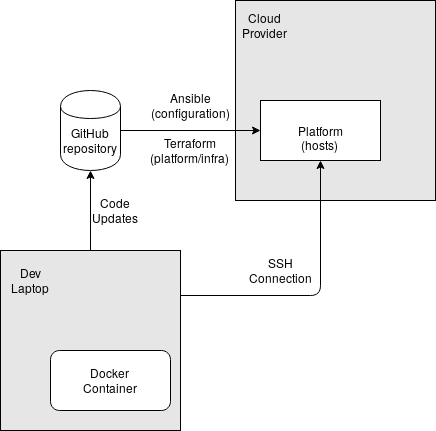
\includegraphics{../images/infra_flow.png}
   \caption{The pipeline flow.}
\end{figure}

Consider the following diagram {myFig4} as we discuss the tools we'll
use to implement our infrastructure as code and associated
configurations in the cloud provider network.

\section{Packer}

\justify
Using Hashicorp Packer is a great way to nail down the contents of a
machine image before we bring up an instance. Download Packer from the
Hashicorp web site in preparation for the following steps\footnote{\url{https://github.com/bonclay7/aws-amicleaner}}. 
We will focus on creating images for our cloud provider from the
command line. Bear in mind it is also possible to use Terraform to
manage the creation of Packer generated machine images. Generating
machine images on the fly using Terraform would increase our degree of
ephepmerality and immutability.

\subsection{Packer Example Configuration for AWS}

Here is an example of how to set up a JSON file to build a Packer image
in AWS. Save the contents of this file into
`packer/aws-debian-host.json`:

\justify
\begin{mybox}{\thetcbcounter: aws-debian-host.json}
	\lstinputlisting{code/aws-debian-host.json}
\end{mybox}

\subsection{Packer Example Configuration for GCP}

\justify
Here is an example of how to set up a JSON file to build a Packer image
in Google Compute. Save the contents of this file into
`packer/gcp-debian-host.json`:

\justify
\begin{mybox}{\thetcbcounter: gcp-debian-host.json}
	\lstinputlisting{code/gcp-debian-host.json}
\end{mybox}


\subsection{Validating Packer JSON Files}

\justify
Once the JSON files are created and saved in the packer directory, we
can use the packer tool to validate them. Type
packer validate \textless{}filename\textgreater{} to validate each new
JSON file. This gives you a chance to find and fix any errors before the
next step, the build phase.

\justify
Note that your validation commands may fail if the cloud provider
credentials have not been configured at this point.

\subsection{Building Images with Packer}

\justify
Finally, we are ready to build our new images. Try typing
packer build \textless{}filename\textgreater{} to create the image. You
should see output similar to the following, but with a unique AMI ID.

\begin{mybox}{\thetcbcounter: packer build}
Build 'amazon-ebs' finished.

==> Builds finished. The artifacts of successful builds are:
--> amazon-ebs: AMIs were created:
    us-west-2: ami-0e9e6427509a9d0b5
\end{mybox}

\justify
The AMI ID "ami-0e9e6427509a9d0b5" is now a usable image that we can
include in our Terraform builds.

\subsection{Removing Packer Images from Cloud Provider}

\justify
You may want to remove the images from AWS/GCP since storing them incurs
additional cost, whether they are in use or not\footnote{\url{https://registry.terraform.io/modules/trussworks/lambda-packerjanitor/aws/1.0.0}}
.
\justify
To remove stale machine images from AWS, you may try a tool such as
aws-amicleaner\footnote{\url{https://www.terraform.io/intro/index.html}}
, which is available to be installed via Python/pip as well as from the
GitHub repository for the project.

\jusitfy
Another AWS specfic tool is "lambda-packerjanitor" from Trusworks.

\section{Terraform}

\justify
Terraform, created by Hashicorp in 2014, is a tool for building, changing, and versioning infrastructure safely and efficiently . Install the latest version of Terraform in preparation for the activities that follow.

\justify
Consider the relevant Terraform files that we will include in our
projects.

\begin{figure}[!htb]
	
\begin{tikzpicture}[>=latex,line join=bevel,]
  \pgfsetlinewidth{1bp}
%%
\pgfsetcolor{black}
  % Edge: home -> devsecops
  \draw [->] (184.5bp,215.83bp) .. controls (184.5bp,208.13bp) and (184.5bp,198.97bp)  .. (184.5bp,180.41bp);
  % Edge: devsecops -> aws
  \draw [->] (184.5bp,143.83bp) .. controls (184.5bp,136.13bp) and (184.5bp,126.97bp)  .. (184.5bp,108.41bp);
  % Edge: aws -> main
  \draw [->] (146.4bp,71.831bp) .. controls (125.07bp,61.661bp) and (98.412bp,48.951bp)  .. (67.217bp,34.077bp);
  % Edge: aws -> out
  \draw [->] (169.11bp,71.831bp) .. controls (162.01bp,63.454bp) and (153.45bp,53.353bp)  .. (139.1bp,36.413bp);
  % Edge: aws -> tfvars
  \draw [->] (199.89bp,71.831bp) .. controls (206.99bp,63.454bp) and (215.55bp,53.353bp)  .. (229.9bp,36.413bp);
  % Edge: aws -> var
  \draw [->] (227.81bp,73.842bp) .. controls (254.87bp,63.747bp) and (290.05bp,50.625bp)  .. (329.25bp,36.001bp);
  % Node: home
\begin{scope}
  \definecolor{strokecol}{rgb}{0.0,0.0,0.0};
  \pgfsetstrokecolor{strokecol}
  \draw (215.5bp,252.0bp) -- (212.5bp,256.0bp) -- (191.5bp,256.0bp) -- (188.5bp,252.0bp) -- (153.5bp,252.0bp) -- (153.5bp,216.0bp) -- (215.5bp,216.0bp) -- cycle;
  \draw (184.5bp,234.0bp) node {/home};
\end{scope}
  % Node: devsecops
\begin{scope}
  \definecolor{strokecol}{rgb}{0.0,0.0,0.0};
  \pgfsetstrokecolor{strokecol}
  \draw (255.0bp,180.0bp) -- (252.0bp,184.0bp) -- (231.0bp,184.0bp) -- (228.0bp,180.0bp) -- (114.0bp,180.0bp) -- (114.0bp,144.0bp) -- (255.0bp,144.0bp) -- cycle;
  \draw (184.5bp,162.0bp) node {/home/devsecops};
\end{scope}
  % Node: aws
\begin{scope}
  \definecolor{strokecol}{rgb}{0.0,0.0,0.0};
  \pgfsetstrokecolor{strokecol}
  \draw (227.5bp,108.0bp) -- (224.5bp,112.0bp) -- (203.5bp,112.0bp) -- (200.5bp,108.0bp) -- (141.5bp,108.0bp) -- (141.5bp,72.0bp) -- (227.5bp,72.0bp) -- cycle;
  \draw (184.5bp,90.0bp) node {terraform};
\end{scope}
  % Node: main
\begin{scope}
  \definecolor{strokecol}{rgb}{0.0,0.0,0.0};
  \pgfsetstrokecolor{strokecol}
  \draw (67.0bp,36.0bp) -- (0.0bp,36.0bp) -- (0.0bp,0.0bp) -- (67.0bp,0.0bp) -- cycle;
  \draw (33.5bp,18.0bp) node {main.tf};
\end{scope}
  % Node: out
\begin{scope}
  \definecolor{strokecol}{rgb}{0.0,0.0,0.0};
  \pgfsetstrokecolor{strokecol}
  \draw (162.0bp,36.0bp) -- (85.0bp,36.0bp) -- (85.0bp,0.0bp) -- (162.0bp,0.0bp) -- cycle;
  \draw (123.5bp,18.0bp) node {output.tf};
\end{scope}
  % Node: tfvars
\begin{scope}
  \definecolor{strokecol}{rgb}{0.0,0.0,0.0};
  \pgfsetstrokecolor{strokecol}
  \draw (311.0bp,36.0bp) -- (180.0bp,36.0bp) -- (180.0bp,0.0bp) -- (311.0bp,0.0bp) -- cycle;
  \draw (245.5bp,18.0bp) node {terraform.tfvars};
\end{scope}
  % Node: var
\begin{scope}
  \definecolor{strokecol}{rgb}{0.0,0.0,0.0};
  \pgfsetstrokecolor{strokecol}
  \draw (425.5bp,36.0bp) -- (329.5bp,36.0bp) -- (329.5bp,0.0bp) -- (425.5bp,0.0bp) -- cycle;
  \draw (377.5bp,18.0bp) node {variables.tf};
\end{scope}
%
\end{tikzpicture}


	\caption{Terraform related files and folders.}
\end{figure}

\subsection{terraform.tfvars}

When working with AWS as cloud provider, life gets a bit easier if you
save a copy of your console credentials in a file called
terraform.tfvars as seen in the next example. You must be very careful
not to commit these credentials to GitHub! Adding the line
terraform.tfvars to your .gitignore file at the top level of your lab
repository helps a lot. Keeping track of your credentials is very
important!

\justify
An example of a local terraform.tfvars file follows. Remember that this
file will never be checked into GitHub or any other revision control
toolset.

\begin{Shaded}
   \begin{Highlighting}[]
      \ExtensionTok{aws_access_key}\NormalTok{ = AKIAJCQ6WHUXVOKZ8RQQ}
      \ExtensionTok{aws_secret_key}\NormalTok{ = q27qR8fwdHLUh7WOEH3JVd2VHjfRlQs1jlhhbZbQ}
   \end{Highlighting}
\end{Shaded}


\subsection{main.tf}

\justify
This file will contain the bulk of our Terraform configurations. As with
Python, we have the ability to reference modules, both internal and
exteral. The main.tf file is the place the module references are made.

\begin{Shaded}
   \begin{Highlighting}[]
      \ExtensionTok{module} \StringTok{"security_group"}\NormalTok{ \{}
      \BuiltInTok{source}\NormalTok{  = }\StringTok{"terraform-aws-modules/security-group/aws"}
      \ExtensionTok{version}\NormalTok{ = }\StringTok{"~> 3.0"}

      \ExtensionTok{name}\NormalTok{        = }\StringTok{"DevSecOps"}
      \ExtensionTok{description}\NormalTok{ = }\StringTok{"Security group for the cloud lab"}
      \ExtensionTok{vpc_id}\NormalTok{      = data.aws_vpc.default.id}

      \ExtensionTok{ingress_cidr_blocks}\NormalTok{ = [}\StringTok{"0.0.0.0/0"}\NormalTok{]}
      \ExtensionTok{ingress_rules}\NormalTok{       = [}\StringTok{"http-80-tcp"}\NormalTok{, }\StringTok{"all-icmp"}\NormalTok{, }\StringTok{"ssh-tcp"}\NormalTok{]}
      \ExtensionTok{egress_rules}\NormalTok{        = [}\StringTok{"all-all"}\NormalTok{]}
      \NormalTok{\}}
   \end{Highlighting}
\end{Shaded}

\justify
We can also designate our data sources in the main.tf file. Consider the
following Terraform data sources. These AWS data sources reference our
Virtual Private Cloud (VPC) and provider-assigned IPv4 Subnets.

\begin{Shaded}
   \begin{Highlighting}[]
      \ExtensionTok{data} \StringTok{"aws_vpc"} \StringTok{"default"}\NormalTok{ \{}
      \ExtensionTok{default}\NormalTok{ = true}
      \NormalTok{\}}

      \ExtensionTok{data} \StringTok{"aws_subnet_ids"} \StringTok{"all"}\NormalTok{ \{}
      \ExtensionTok{vpc_id}\NormalTok{ = data.aws_vpc.default.id}
      \NormalTok{\}}
   \end{Highlighting}
\end{Shaded}


\subsection{outputs.tf}\label{outputs.tf}}

\justify
We can display or export the resources we've created in main.tf using a
file known as outputs.tf. We may have a need to display the IP address
of host instances we've just created, which is helpful to a user who
needs to log in. We may also wish to make values available to other
Terraform modules.

\justify
Consider the following output declarations from our example code.

\begin{Shaded}
   \begin{Highlighting}[]
      \ExtensionTok{output} \StringTok{"web_public_ip"}\NormalTok{ \{}
      \ExtensionTok{description}\NormalTok{ = }\StringTok{"Public IPs assigned to the web instance"}
      \ExtensionTok{value}\NormalTok{       = aws_instance.web.public_ip}
      \NormalTok{\}}

      \ExtensionTok{output} \StringTok{"kali_public_ip"}\NormalTok{ \{}
      \ExtensionTok{description}\NormalTok{ = }\StringTok{"Public IPs assigned to the kali instance"}
      \ExtensionTok{value}\NormalTok{       = aws_instance.kali.public_ip}
      \NormalTok{\}}
   \end{Highlighting}
\end{Shaded}


\subsection{variables.tf}

\justify
The variables.tf file is another common file seen in projects in AWS,
GCP and other cloud providers. It contains declarations of variables,
and often values for variables as well, that will be used in the main.tf
file. As an example there might be region information or even the name
of the image we created previously with Packer.

\justify
Consider the following example. Here we declare a "region" variable in
the file variables.tf.

\begin{Shaded}
   \begin{Highlighting}[]
      \ExtensionTok{variable} \StringTok{"region"}\NormalTok{ \{}
      \ExtensionTok{description}\NormalTok{ = }\StringTok{"AWS region to launch servers."}
      \ExtensionTok{default}\NormalTok{     = }\StringTok{"us-west-2"}
      \NormalTok{\}}
   \end{Highlighting}
\end{Shaded}


\subsection{Verification}

\justify
Terraform has some commands, validate and fmt (short for "format") that
we can use to syntactically verify our configuration before sending it
off to the cloud provider to act upon. Validating your Terraform files
is as easy as typing terraform validate in the directory the files exist
in.

\begin{Shaded}
   \begin{Highlighting}[]
      \ExtensionTok{user@devsecops}\NormalTok{::~/workspace/rapid_secdev_framework/aws$ terraform validate}
      \ExtensionTok{Success}\NormalTok{! The configuration is valid.}
   \end{Highlighting}
\end{Shaded}

To get your Terrform files into a clean standard format, the
terraform fmt command works well. There is also the option to do this
formatting from inside the VSCode window on a per-file basis.


\subsection{Plan}

First we will will create a "plan" in preparation for application.

\begin{Shaded}
   \begin{Highlighting}[]
      \ExtensionTok{user@devsecops}\NormalTok{::~/workspace/rapid_secdev_framework/aws$ terraform plan -out franklin.out}
      \ExtensionTok{Refreshing}\NormalTok{ Terraform state in-memory prior to plan...}
      \ExtensionTok{The}\NormalTok{ refreshed state will be used to calculate this plan, but will not be}
      \ExtensionTok{persisted}\NormalTok{ to local or remote state storage.}

      \ExtensionTok{data.aws_vpc.default}\NormalTok{: Refreshing state...}
      \ExtensionTok{data.aws_subnet_ids.all}\NormalTok{: Refreshing state...}

      \ExtensionTok{------------------------------------------------------------------------}

      \ExtensionTok{An}\NormalTok{ execution plan has been generated and is shown below.}
      \ExtensionTok{Resource}\NormalTok{ actions are indicated with the following symbols:}
      \ExtensionTok{+}\NormalTok{ create}


      \ExtensionTok{Plan}\NormalTok{: 8 to add, 0 to change, 0 to destroy.}

      \ExtensionTok{------------------------------------------------------------------------}

      \ExtensionTok{This}\NormalTok{ plan was saved to: franklin.out}

      \ExtensionTok{To}\NormalTok{ perform exactly these actions, run the following command to apply:}
      \ExtensionTok{terraform}\NormalTok{ apply }\StringTok{"franklin.out"}
   \end{Highlighting}
\end{Shaded}

\subsection{Apply}

The apply action is where the rubber meets the proverbial road. This
action will transmit our configurations to the cloud provider and
allocate the necessary resources to stand up our environment.

With our plan in place, we can now "apply" that plan to the cloud
provider. This can take a counsiderable amount of time, depending on the
complexity of the desired configuration. Note that Terraform will prompt
you to enter "yes" before it will proceed.

\begin{Shaded}
   \begin{Highlighting}[]
      \ExtensionTok{user@devsecops}\NormalTok{::~/workspace/rapid_secdev_framework/aws$ terraform apply}
      \ExtensionTok{data.aws_vpc.default}\NormalTok{: Refreshing state...}
      \ExtensionTok{data.aws_subnet_ids.all}\NormalTok{: Refreshing state...}

      \ExtensionTok{An}\NormalTok{ execution plan has been generated and is shown below.}
      \ExtensionTok{Resource}\NormalTok{ actions are indicated with the following symbols:}
      \ExtensionTok{+}\NormalTok{ create}

      \ExtensionTok{Plan}\NormalTok{: 8 to add, 0 to change, 0 to destroy.}

      \ExtensionTok{Do}\NormalTok{ you want to perform these actions?}
      \ExtensionTok{Terraform}\NormalTok{ will perform the actions described above.}
      \ExtensionTok{Only} \StringTok{'yes'}\NormalTok{ will be accepted to approve.}

      \ExtensionTok{Enter}\NormalTok{ a value: yes}

      \ExtensionTok{Apply}\NormalTok{ complete! Resources: 8 added, 0 changed, 0 destroyed.}

      \ExtensionTok{Outputs}\NormalTok{:}

      \ExtensionTok{kali_public_ip}\NormalTok{ = 34.221.121.11}
      \ExtensionTok{web_public_ip}\NormalTok{ = 54.186.129.232}
   \end{Highlighting}
\end{Shaded}

\section{Ansible}

\justify
Environments where you have a set of repeatable configuration steps can
be deployed more quickly with Ansible. Building a set of good Ansible
playbooks over team means you can pick and choose the most useful
patterns in future projects. A true force multiplier.

single: Ansible

\hypertarget{installing-ansible}{%
   \subsubsection{Installing Ansible}\label{installing-ansible}}

Simply adding "ansible" to python/requirements.txt will make Ansible
available in our Docker containers. Now when we type make docker, pip
will take care of the installation for us. Then we can experiment with
Ansible playbook runs.

\hypertarget{ansible-playbooks}{%
   \subsubsection{Ansible Playbooks}\label{ansible-playbooks}}

Ansible breaks down it's execution runs into discrete workflows known as
playbooks. Playbooks are executed on the target hosts to implement
configurations. It's quite useful to be able to kick off a playbook run
on the taget host every 15 minutes. This is a direct example of
Continuous Deployment in action. If somethings changes in the GitHub
repository, we want that to propagate out to the targets and the latest
configuration to be applied to the server. We can also deploy a newer
version of an application and then stop and start the applicationto
effect the change.

Ansible playbooks break down target hosts into groupings known as roles.

\hypertarget{testing-ansible-playbooks}{%
   \subsubsection{Testing Ansible
      Playbooks}\label{testing-ansible-playbooks}}

There is a test framework known as "molecule" that can be used to test
ansible playbooks.

single: Molecule

\begin{Shaded}
   \begin{Highlighting}[]
      \NormalTok{$ }\ExtensionTok{molecule}\NormalTok{ init role -r logfwd}
      \ExtensionTok{--}\OperatorTok{>}\NormalTok{ Initializing new role logfwd...}
      \ExtensionTok{Initialized}\NormalTok{ role in /ansible/roles/logfwd successfully.}
   \end{Highlighting}
\end{Shaded}


\section{Ansible Vault}

\justify
Vault is a tool that is included with Ansible. You may notice that
ansible-vault is a symlink back to ansible on your system. Vault is an
easy way to protect secrets using AES-256 encryption in your GitHub
repositories. For example, we can use it to secure data at rest in a
repository, or protect system configuration data as it transits through
our pipelines out to our cloud providers.

single: AES-256 single: Vault

\subsection{Encrypting a File with Vault}

\justify
Let's try encrypting a file... using another file! Create a text file
with some random contents. For example, create a file in your home
directory called my\_dog.txt with the following contents:

\begin{Shaded}
   \begin{Highlighting}[]
      \ExtensionTok{My}\NormalTok{ dog has fleas.}
   \end{Highlighting}
\end{Shaded}

Now we can encrypt some data using this file as the encryption key. For
the sake of example, let's assume we have a file called
data\_to\_protect.txt that we would like to encrypt.

\begin{Shaded}
   \begin{Highlighting}[]
      \ExtensionTok{ansible-vault}\NormalTok{ encrypt --vault-password-file ~/my_dog.txt data_to_protect.txt}
   \end{Highlighting}
\end{Shaded}

Now when we view the data\_to\_protect.txt file, we can see it has been
encrypted and appears as a long series of seemingly nonsense characters.


\subsection{Decrypting a File with Vault}

\justify
At some point, we are going to want to decrypt our data so it becomes
usable, we can perform operations on it, and so on. As long as we keep
or recreate the original key file on our host, or create an identical
copy of the key file some some target/remote host, we will be able to
decrypt the data. This is quite useful to us indeed, when it comes to
protecting our data.

\begin{Shaded}
   \begin{Highlighting}[]
      \ExtensionTok{ansible-vault}\NormalTok{ decrypt --vault-password-file ~/my_dog.txt data_to_protect.txt}
   \end{Highlighting}
\end{Shaded}

\clearpage

\section{Tool Directory Structure}

Files and folders relevant to this chapter are organized as shown below.

\begin{description}
   \item[digraph folders \{]
         "devsecops" {[}shape=folder{]}; "ansible" {[}shape=folder{]}; "aws"
         {[}shape=folder{]}; "packer" {[}shape=folder{]}; "aws-debian-host.json"
         {[}shape=rect{]}; "gcp-debian-host.json" {[}shape=rect{]}; "main.tf"
         {[}shape=rect{]}; "outputs.tf" {[}shape=rect{]}; "terraform.tfvars"
         {[}shape=rect{]}; "variables.tf" {[}shape=rect{]}; "devsecops"
         -\textgreater{} "ansible"; "devsecops" -\textgreater{} "aws";
         "devsecops" -\textgreater{} "packer"; "aws" -\textgreater{} "main.tf";
         "aws" -\textgreater{} "outputs.tf"; "aws" -\textgreater{}
         "terraform.tfvars"; "aws" -\textgreater{} "variables.tf"; "packer"
         -\textgreater{} "aws-debian-host.json"; "packer" -\textgreater{}
         "gcp-debian-host.json";
\end{description}

\}

\chapter{The Lab}

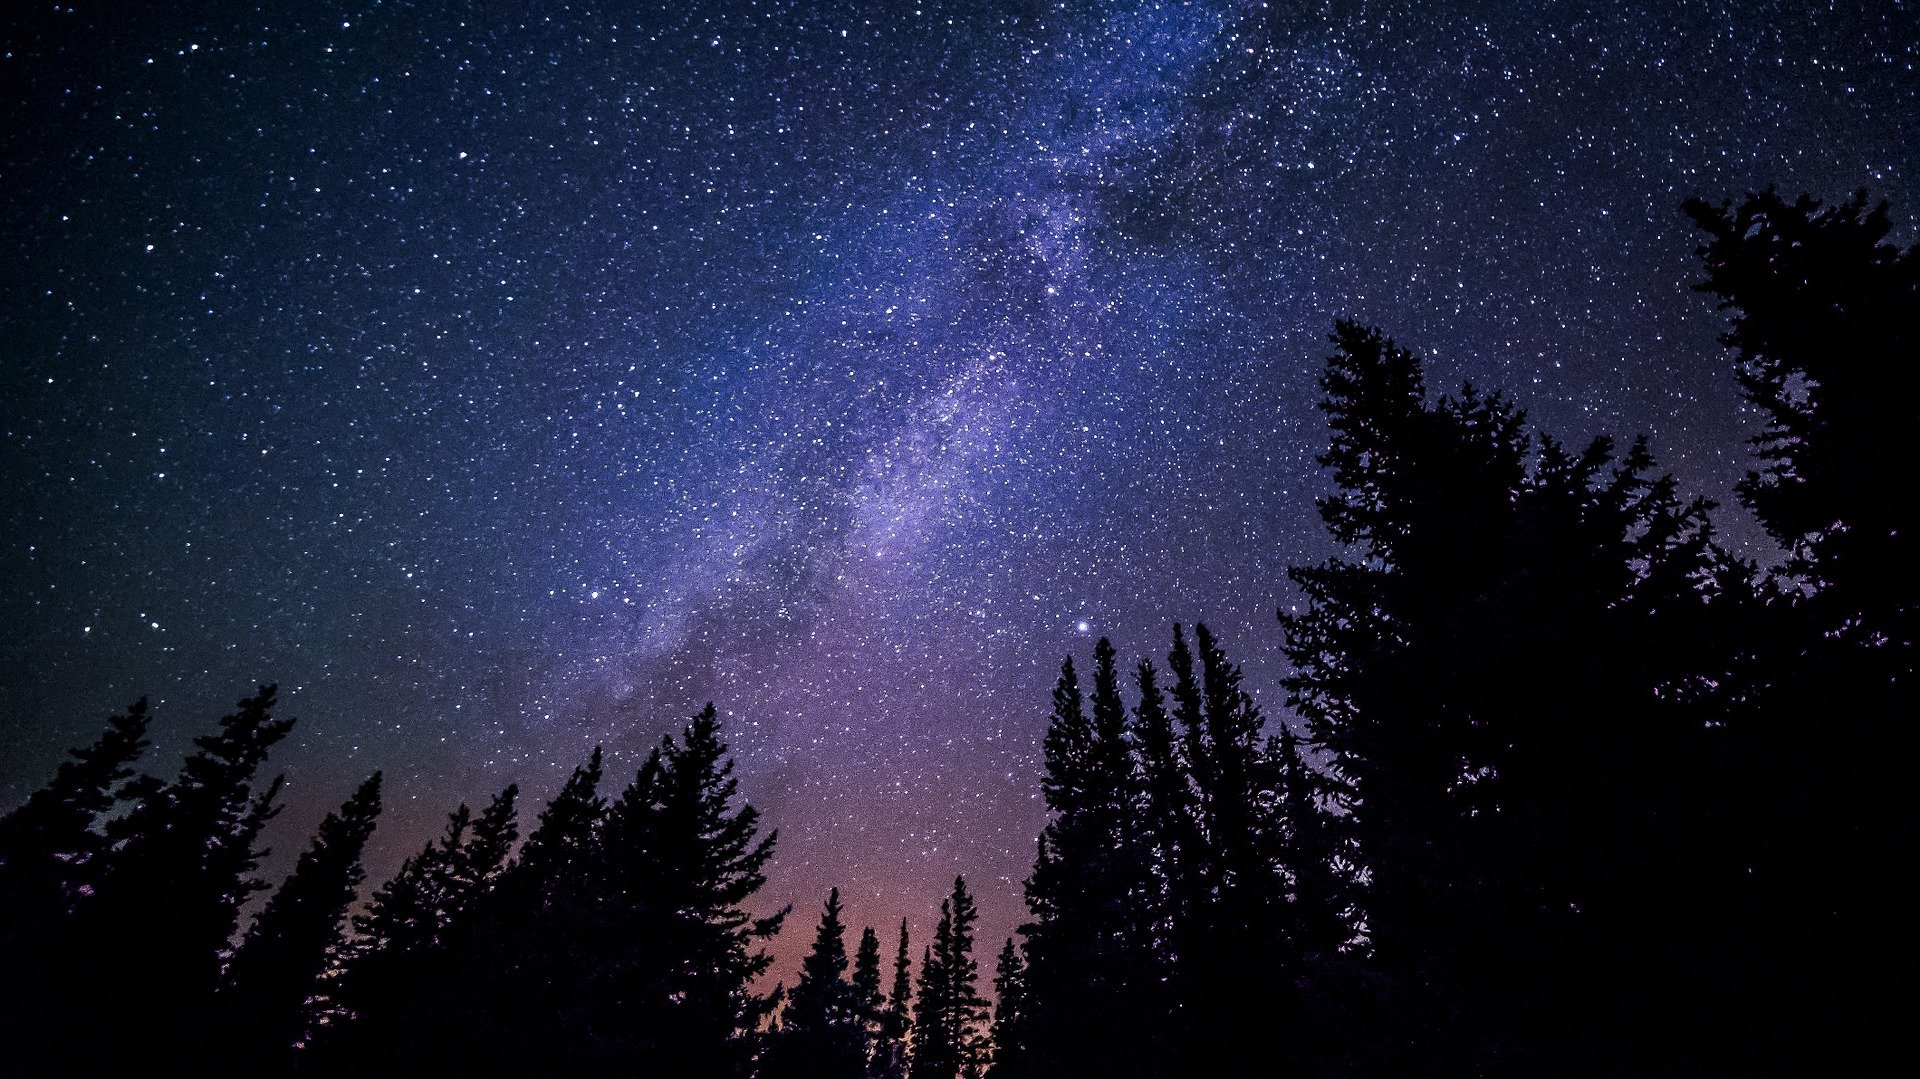
\includegraphics[scale=0.20]{images/milky-way-984050_1920.jpg}
\justify{}
We've reached the point where it's time to assemble all our functional
blocks into a proper lab using resources of a cloud service provider.

\section{Getting Started}

\subsection{Setting up AWS}
\justify{}
Establish an AWS account.

\subsection{Install Docker}
\justify{}
Install Docker on your local machine. Create a Dockerfile and
docker-compose.yml.

\subsection{Configure Project Repository}
\justify{}
Create a GitHub repo for our project. Clone the repo. Copy the
Dockerfile and docker-compose.yml into the new project directory. Create
a branch. Commit the files to the branch and push to repo on GitHub.
Merge the branch, then do a pull to sync your local clone.

\subsection{Configure Testing}
\justify{}
Walk through the steps of adding GitHub Actions that will validate the
Terraform we will be writing to establish our lab infrastructure.

\section{Infrastructure}

\subsection{Lab Diagram}
\justify{}
Let's take a look at the lab environment we intend to create.

\subsection{Add a Makefile}
\justify{}
Add a Makefile that will respond to the ``make docker'' command.

\subsection{Create a Host with Packer}

\subsection{Write Some Terraform Files}

\subsection{Applications}

\subsection{Python Application}

\subsection{Extras}

\subsection{Add a Firewall}
\justify{}
Every keep needs walls around the castle to stop the bad guys from
getting in. The Palo Alto VM-300 series firewall is available as an
image that can be installed in AWS or GCP as desired.


% backmatter: appendix, bibliography, index, postface
\backmatter
\bibliographystyle{apalike}
\nocite{*}
\printindex
\bibliography{backmatter/mybib}
theend

%%% front cover, spline, back cover
% front_cover

\end{document}

